\documentclass[11pt, a4paper, twoside]{report}
\usepackage [T1] {fontenc}
\usepackage[latin1]{inputenc}
\usepackage{algorithmic}
\usepackage{graphicx}
\usepackage{parskip}
\usepackage{amsmath, amsthm, amssymb}
\usepackage{subfigure}
\usepackage{url}
\usepackage{tikz}
\usepackage{verbatim} 
\usepackage{listings} 
\usepackage{fancyvrb} \fvset{frame=single, fontsize=\small}
%\usepackage{nomencl}
\usepackage[pdftex, bookmarks=true, linkbordercolor={0.8 0.8 0.8}]{hyperref}
%\graphicspath{{./img}}
\usetikzlibrary{trees}
\usetikzlibrary{shapes}
\newtheoremstyle{myExStyle}% name
     {8pt}%      Space above
     {8pt}%      Space below
     {}%         Body font
     {}%         Indent amount (empty = no indent, \parindent = para indent)
     {\bfseries}% Thm head font
     {:}%        Punctuation after thm head
     {.5em}%     Space after thm head: " " = normal interword space;
           %       \newline = linebreak
     {}%         Thm head spec (can be left empty, meaning `normal')


\newtheorem{myDefinition}{Definition}
\theoremstyle{myExStyle}
\newtheorem{myExample}{Example}
%\addtolength{\oddsidemargin}{-.7in}
\addtolength{\evensidemargin}{-1.1in}
\addtolength{\textwidth}{1.1in}
\addtolength{\topmargin}{-.55in}
%\addtolength{\bottommargin}{-.6in}
\addtolength{\textheight}{0.8in}
\addtolength{\footskip}{0.25in}
%\pdfpagewidth 8.26in
%\pdfpageheight 11.7in
%\makenomenclature
% Different font in captions
\newcommand{\captionfonts}{\small\itshape}
\makeatletter  % Allow the use of @ in command names
\long\def\@makecaption#1#2{%
  \vskip\abovecaptionskip
  \sbox\@tempboxa{{\captionfonts #1: #2}}%
  \ifdim \wd\@tempboxa >\hsize
    {\captionfonts #1: #2\par}
  \else
    \hbox to\hsize{\hfil\box\@tempboxa\hfil}%
  \fi
  \vskip\belowcaptionskip}
\makeatother   % Cancel the effect of \makeatletter
\begin{document}

%\renewcommand{\nomname}{Glossary}


\nomenclature{\textbf{AST}}{\textbf{A}bstract \textbf{S}yntax \textbf{T}ree. A two-dimensional tree which encode the structure of the the input symbols.}


\nomenclature{\textbf{W3C}}{\textbf{W}orld \textbf{W}ide \textbf{W}eb
\textbf{C}onsortium. An international standards organisation for the World Wide Web.}

\nomenclature{\textbf{EBNF}}{\textbf{E}xtended \textbf{B}ackus \textbf{N}aur \textbf{F}orm. A metasyntax notation used to express context-free grammars}

\nomenclature{\textbf{ANTLR}}{\textbf{AN}other \textbf{T}ool for \textbf{L}anguage \textbf{R}ecognition. A predicated-LL(k) parser generator that handles lexers, parsers, and tree parsers.}

\nomenclature{\textbf{Production}}{A grammar spesification rule, either terminal or non-terminal.}

\nomenclature{\textbf{MQL}}{\textbf{M}ARS \textbf{Q}uery \textbf{L}anguage. The relational algebra language of
MARS}

\nomenclature{\textbf{MARS}}{A search engine platform under development at Fast Search \& Transfer}

\nomenclature{\textbf{Tainting Dependencies}}{A novel XQuery to MQL translation method developed as a part of this
Master's thesis. See Chapter \ref{chapter:translation}}

\nomenclature{\textbf{TD}}{See \textbf{Tainting Dependencies}}

\nomenclature{\textbf{Loop Lifting}} {A XQuery to relational algebra translation method developed by Torsten
Grunst and Jens Teubner. See Section \ref{sect:theory:loop_lifting}.}

\nomenclature{\textbf{DAG}} {\textbf{D}irected \textbf{A}syclic \textbf{G}raph.}

\nomenclature{\textbf{FLWOR}} {\textbf{f}or, \textbf{l}et, \textbf{w}here, \textbf{o}rder by, \textbf{r}eturn. A
XQuery expression with loop semantics. See Section \ref{sect:theory:xquery:Flwor}.}

\nomenclature{\textbf{normalised}, relation} {A relation without redundancies.}

\nomenclature{\textbf{normalised}, XQuery} {See XQuery Core, Section \ref{sect:theory:xquery:XQcore}.}

\nomenclature{\textbf{DOM}}{}



%\begin{titlepage}
%\title{Development of an XQuery full-text parser}
%\author{Andreas Ravnestad, Mads Nyborg}
%\end{titlepage}

%\newpage

\thispagestyle{empty}
\begin{center}
  \vspace*{1cm}
  {\Huge \bf Development of an XQuery parser with full-text extensions}

  \vspace*{2cm}
  {\LARGE\bf Mads Nyborg, Andreas Ravnestad}

  \vfill

  \vspace*{0.9cm}
  
  % Put your university logo here if you wish.
   \begin{center}
   
\includegraphics[width=0.15\textwidth]{img/logo_ntnu}
   \end{center}

  {
	  Department of Computer and Information Science\\
	  Norwegian University of Science and Technology\\
	  Norway\\
	  \today}

\end{center}
%\newpage

%\mbox{}

\chapter*{Abstract}

XQuery is a flexible language for querying XML data across a variety of storage
methods. This Master's thesis is a part of iAD, an ongoing research effort in next generation information access
solutions. iAD is hosted by Fast Search \& Transfer, a company at the time developing their next search engine
platform MARS.

The goal of this thesis is to investigate the posibilities for utilising XQuery as a query interface to MARS. And
specififcally to find a way to translate XQuery to the MARS relational algebra language MQL.
\marginpar{\scriptsize litt skummelt? }

The project resulted in the develpment of a novel translation method, dubbed ``Tainting Dependencies''.
Based on this method, a proof of concept has been implemented for generation of algebra.

This method of translation which produces algebra significantly less complex than that produced by an existing
method dubbed ``Loop Lifting''. These methods are then compared and evaluated through discussion.

\textbf{\LARGE TODO:} TJeeeeeeeeh

\newpage

%\mbox{}

\chapter*{Preface}

This thesis was written at the Department of Computer and Informations Science
(IDI) at the Norwegian University of Science and Techology (NTNU) during the
spring semester of 2008. The assignment was given by and written for the
Information Access Distruption centre (iAD). The supervisors of this project
has been Svein Erik Bratsberg at NTNU and \O ystein Torbj\o rnsen at Fast
Search \& Transfer.

We would like to thank Svein Erik Bratsberg for feedback and proof reading of
this report. Additionally we would also like to thank \O ystein Torbj\o rnsen
for taking time from his busy schedule giving guidance, feedback and teaching
us about the workings of MARS.

\begin{verbatim}







\end{verbatim}
\begin{center}

Trondheim, \today

\begin{verbatim}


\end{verbatim}
Andreas Ravnestad \verb!                      ! Mads Nyborg
\end{center}


\newpage

%\mbox{}

\tableofcontents

%\listoffigures

%\printnomenclature


\chapter{Introduction}
\label{chapter:introduction}
% \begin{itemize}
%   \item \textbf{\LARGE TODO:} Acknowledgements i kap f\o r?
%   \item motiv for oppgave
%   \item vi har funnet opp ``Tainting Dependencies'' -- en metode for \aa~oversette XQuery til MQL
%   \item vi har sammenlignet mot Loop Lifting (Pathfinder) og det viser seg \aa~v\ae re god stemning
%   \item \ldots
%   \item \ldots 
% 
% \end{itemize}


The search engines of today are capable of finding relevant documents based
on simple search terms as well as weighting and ranking schemes of varying
complexity. However, few are capable of joining several query results,
performing structural queries, and filtering by complex full-text expressions
in a single unified query operation. 

XQuery is an XML query language capable of performing complex nested
queries, extendable with full-text extensions, including linguistics such as
stemming and thesaurus. In theory, XQuery queries can be translated into
relational algebra for execution on a suitable algebra processor engine.

iAd \cite{iadcentre} (Information Access Disruptions) is an ongoing research
effort in ``next generation information access solutions'', in which this
project partake. Our specific goal is thus to develop a method of
translating XQuery queries into relational algebra, and furthermore implement a
proof of concept and compare this to existing technology. 

In chapter \ref{chapter:theory} we will examine XQuery itself in further detail
and investigate the current state of XQuery translator implementations and
research. In chapter \ref{chapter:method} we will detail the tools and methods
used. In chapter \ref{chapter:translation} we will describe our novel
translation method dubbed ``Tainting Dependencies''. Continuing to chapter
\ref{chapter:implementation} we expound on the implementation of a prototype
which serves as a proof of concept. Eventually the results will be
presented and discussed in chapters \ref{chapter:results} and
\ref{chapter:discussion}. Our work is concluded in chapter
\ref{chapter:conclusion}, and we propose future work and improvements in
chapter \ref{chapter:future}.



\textbf{\LARGE TODO:}Ting n\aa r vi g\aa r igjennom rapporten igjen:
\begin{itemize}
  \item count tar ingen /trenger ikke ta noen parametere
  \item hhjoin([] []\ldots = cross()
  \item skrive inprocedings greier for pathfinderartikler
\end{itemize}


%THEORY
\chapter{XQuery -- The XML Query Language}
In this chapter we will outline the basics of the XQuery language as well as the
current state of research and implementations. 

\section{XQuery}

XQuery is a query language developed by the XML Query working group of W3C.
Version 1.0\cite{w3c00} became a W3C Recommendation January 2007. It was designed as a
response to an emerging task: to intelligently express queries in theincreasing
amounts of information stored, exchanged and presented using XML. The language
is derived from Quilt\cite{quilt_queryLanguage}.


\begin{itemize}
\item itroduksjon
\item historie
\item bruksomr\aa der
\item ...
\item atomic vs sequence
\end{itemize}

\subsection{Basics}
\begin{itemize}
  \item sekvenser og ting atomisk, alt je
  \item andre ting som er basisk og ikke surt
\end{itemize}

\subsection{Path Expressions}
\begin{itemize}
\item fra XPath / brukt i mange andre ting (XSLT yeye)
\item ...
\item akser
\item predikat
\item semantikk 
\item eksikveringsorden etc
\end{itemize}

\subsection{FLWOR}

\begin{itemize}
\item motiv
\item ...
\item F L W O R semantikk
\item \^{} --- eksikveringsorden etc
\end{itemize}

\subsection{Binary Operators}

\begin{itemize}
\item motiv
\item ...
\item semantikk
\item hva er sant, hva er usant?
\end{itemize}



\subsection{Evt andre ting fra XQuery vi kommer til \aa~implementere}

\begin{itemize}
\item if then else

\end{itemize}

\subsection{Full Text Extensions}

\begin{itemize}
\item motiv
\item ...
\item semantikk
\item hva har man? ftcontains er kilden...
\end{itemize}
% State of the art, nåværende teknologi og implementasjoner
\section{Current state of XQuery}
\underline{\textbf{\LARGE //TODO:}} Kapittelet m\aa~fylles ut og omstruktureres

There exist a number of XQuery implementations, few however are extended with full text capabilities. This section will briefly present some of the more prominent alternatives.
\subsection{Implementations with full-text extensions}
\subsubsection{Quark / TexQuery}
\begin{figure}[!h]
  \centering
    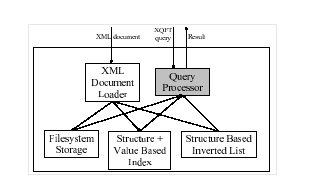
\includegraphics[width=0.5\textwidth]{img/quark_architecture.png}
  \caption{Quark architecture}
\end{figure}
Quark is an experimental full-text search engine capable of indexing and querying XML documents, and it uses the TexQuery query language (see below). Quark was developed as a research project at Cornell University by Jayavel Shanmugasundaram and his associates.
\begin{figure}[!h]
  \centering
    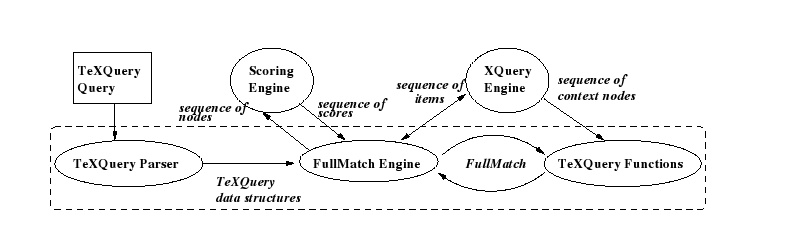
\includegraphics[width=1\textwidth]{img/texquery_architecture.png}
  \caption{TexQuery architecture}
\end{figure}
TexQuery is a query language extending upon Xquery with added full-text search capabilities. These extensions do not necessarily conform to the W3C recommendation, however TexQuery is an early precursor to the current W3C recommendation \cite{TEXQ00}, in whose development Shanmugasundaram actively participates.

\subsubsection{Galatex}
\begin{figure}[!h]
  \centering
    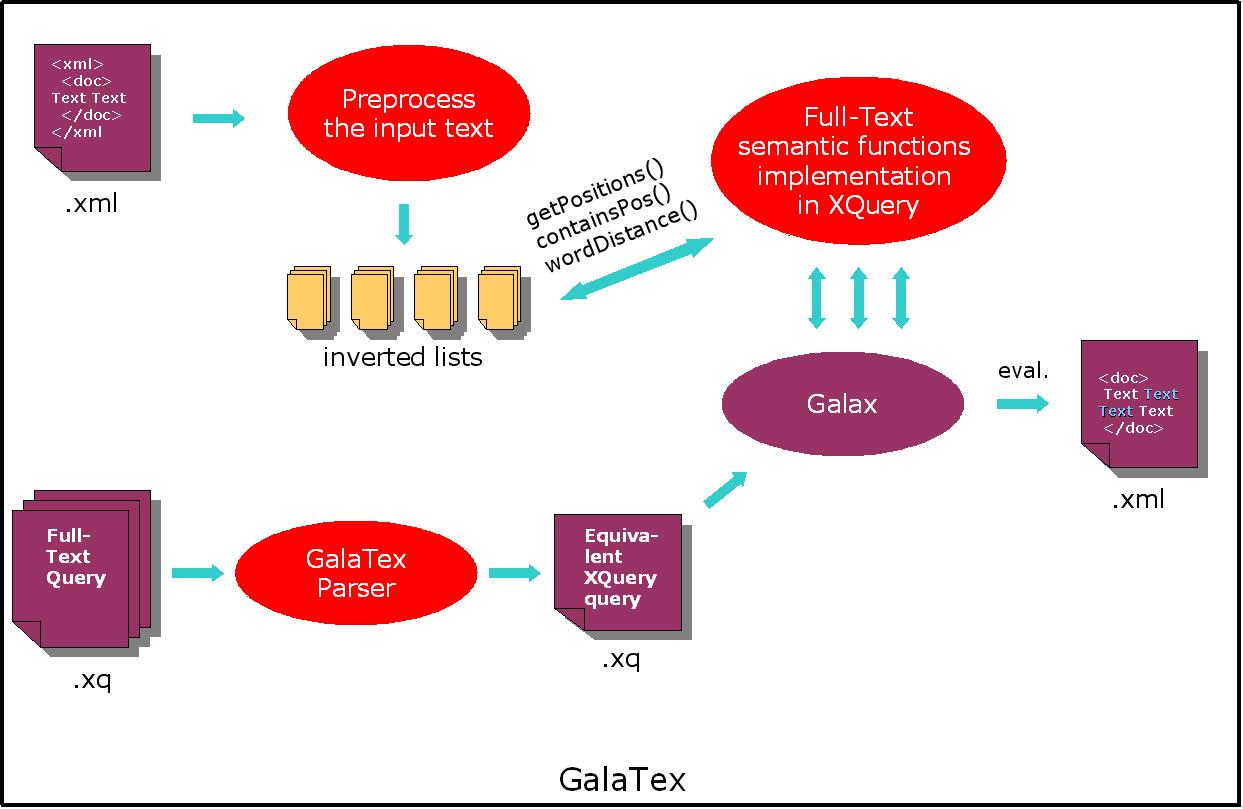
\includegraphics[width=1\textwidth]{img/galatex_architecture.png}
  \caption{Galatex architecture}
\end{figure}
GalaTex is a complete implementation of the Xquery 1.0 and Xpath 2.0
specifications with full-text extensions. GalaTex is an extension of Galax,
which is a generic Xquery engine. The XQFT query is parsed and converted to an
equivalent Xquery query which is passed to the Galax query engine. The GalaTex
source code is licensed under a non-commercial license developed to AT\&{}T 
\footnote{http://www.galaxquery.com/galatex/LICENSE} and is available at the
GalaTex website \cite{galatex}.

\subsubsection{Pathfinder}
\begin{figure}[!h]
  \centering
    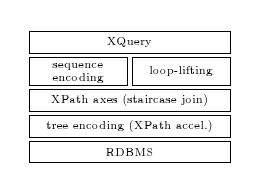
\includegraphics[width=0.5\textwidth]{img/pathfinder_architecture.png}
  \caption{Pathfinder architecture / development stack}
\end{figure}
The Pathfinder project is an XQuery parser running on top of relational database systems, namely MonetDB. The goal of the Pathfinder project is to investigate how relational database technology can be utilized to create a scalable and efficient XQuery implementation. However, the Pathfinder project has, at the current time of writing, no support for full text extensions. A future version of Pathfinder is planned to be capable of emitting SQL code generated from the XQuery parse tree. This illustrates the Pathfinder systems capabilities of interoperating with relational database systems.

Pathfinder is written in C, and the XQuery parser is a generated using standard Flex and Bison compiler generator tools.

\subsubsection{SaXon}
SaXon is an open source XSLT and XQuery processor. It is being actively developed by Michael Kay, and is licensed under the Mozilla Public License (MPL). SaXon conforms to the XSLT 2.0, XQuery 1.0 and XPath 2.0 recommendations by the W3C as of 23rd of january, 2007.

\subsubsection{Natix}
\begin{figure}[!h]
  \centering
    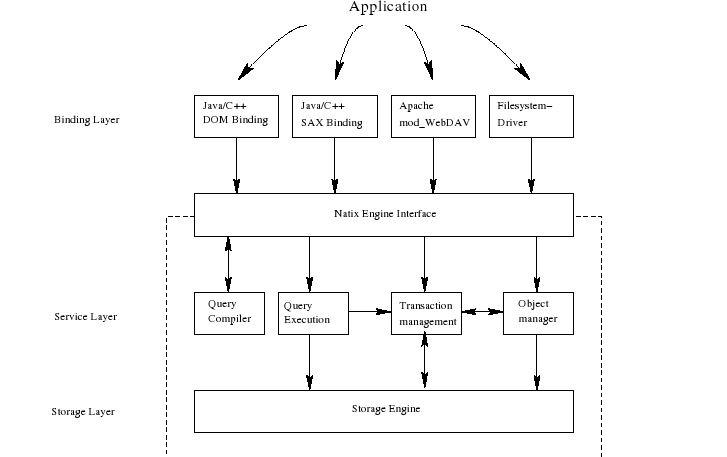
\includegraphics[width=1\textwidth]{img/natix_architecture.png}
  \caption{Natix architecture}
\end{figure}
Natix is an XML database system for persistent storage of XML, and provides access through DOM and SAX interfaces, as well as the option of performing XPath queries.

\section{Summary}
In this chapter, we have presented the basic facets of XQuery and XPath,
especially language features such as FLWOR constructs, path expressions, 
full-text extensions, and precedence. This creates a context for the subsequent
chapters where we will set out to create an XQuery parser with full-text
extensions. 

Further we have investigated existing implementations, both with and without
full-text extensions. These implementations will provide valuable points of
reference for our implementation in the following chapters.

In the next chapter, we will outline the architectural decisions made in this
project.
%\newpage
%\mbox{}

%Relasjonsalgebra
\chapter{Method}
\section{Parser construction}
Writing a parser from scratch was ruled out early for being too time consuming.
Instead it was decided to use tools for compiler and parser construction to
generate a parser from the XQuery 1.0 and XPath 2.0 grammar specifications
developed by the W3C.

\section{Evaluated alternatives}
\subsection{JFlex/CUP}
JFlex and CUP is a versatile combination consisting of JFlex which is a lexer
generator, and CUP which is a parser generator. These tools can be interfaced to
generate a complete parser with a separate lexical analyzer.

JFlex and CUP produces only LALR parsers, and since the W3C has specified an
LL(1) grammar for XQuery 1.0 and XPath 2.0, the combination of JFlex and CUP was
rejected from this project.

\subsection{JavaCC}
JavaCC could have been a viable alternative as it produces LL(k) parsers,
however compared to Antlr its grammar specification syntax deviated so much
from the W3C EBNF syntax, that grammar would have had to be extensively
rewritten.

\subsection{Antlr}
Antlr is a renowned tool for parser generation, and can generate LL(k) parsers.
Additionally, Antlr accepts a grammar specification syntactically very close to
the EBNF used by the W3C. This is the parser generater chosen for our project,
based on the criteria outlined in this section.

\section{Limitations in Antlr}
\subsection{Unicode}
It is important to note, however, that Antlr has limited support for unicode.
In this project this implies that our parser will not accept unicode characters
in the range from and above 0x10000. This will exclude the supplementary
multilingual plane (SMP) range of unicode characters, as well as the
supplementary ideographic plane (SIP) and the supplementary special-purpose
plane (SSP). These are seldomly used, but this is an important limitation
nonetheless. The Antlr developers have indicated that support for this unicode
range will be added in future versions of Antlr.

As a remedy for this situation it is possible to couple an external lexer with
Antlr which will accept unicode characters in the above mentioned character
ranges. For the sake of simplicity this has not been further investigated nor
implemented in this project.

\section{Rewriting the grammar for Antlr syntax conformity}
\subsection{Lexer vs. parser syntax}
The Antlr parser generator can generate parsers and lexers from a single grammar
file. The distinction between terminals and non-terminals is simply a matter of
convention, where terminals are assumed to start with uppercase letters, and
non-terminals are assumed to start with lowercase letters.

In the grammar specified by the W3C, all the productions (terminals and
non-terminals) all start with uppercase letters. Initially this caused some
confusion, because this grammar naturally generated a very big lexer and a very
small and non-functional parser.

This was mitigated by converting non-terminal productions to start with
lowercase letters.

\subsection{Rewriting the W3C 'dash' operator}
In their specification, the W3c uses a dash operator, which has the following
semantic meaning in a grammar (from \cite{w3c03}, section 6):
\begin{quote}
A - B: matches any string that matches A but does not match B.
\end{quote}
This operator is not supported in Antlr, so it was necessary to rewrite
these productions using \emph{semantic predicates} where necessary. Thankfully,
in the original specification, the usage of the dash operator was rather sparse
and only used in trivial productions.

An example of rewriting the dash operator using semantic predicates:
\begin{verbatim}
// Original production
piTarget : Name - (('X' | 'x') ('M' | 'm') ('L' | 'l'));

// Rewritten production using a semantic predicate
piTarget : n=Name { !$n.getText().equalsIgnoreCase("XML") }?;
\end{verbatim}
The original production can be interpreted as ``piTarget can be a Name, but not
`XML', regardless of character casing''. The syntactic predicate will imitate
this behaviour using the method equalsIgnoreCase(). As can be seen from this
example, a semantic predicate is simply any kind of boolean Java expression.
This is a flexible solution, because the boolean expression can be wrapped in a
method with boolean return type, which for example then can be placed inside a
@members { } clause in the grammar file, or even as a static method in an
external class. This makes it possible to add complex grammar logic without
disturbing grammar brevity, if necessary.

\subsection{Grammar LL(1) conformity}
The grammar specification given by W3C is in a very compact and non-verbose
form, annoted with links to certain constraints and issues that need to be kept
in mind by anyone seeking to write a parser for XQuery and XPath. Here we will
list these constraints and briefly explain their implications for the parser.

\begin{itemize}
  \item 
\end{itemize}

\subsection{Reserved keywords}
A particular feature in XQuery is the lack of reserved keywords. This creates a
series of problems when a lexer based on the verbatim grammar specification from
the W3C is trying to recognize tokens. The culprit is the ambiguously defined
terminal symbols. Some of the base character tokens intersect with each other
and makes it hard if not impossible for the lexer to distinguish two different
tokens composed of different token fragments with intersecting characters.

One possible solution to this problem was to eliminate ambiguities in the lexer.
This approach was tried by finding and removing duplicate characters from token
fragments, and then generalizing the tokens and adding semantic predicates to
check for illegal and/or missing characters.

TODO: example

TODO: result (also note in conclusion)

\subsection{Nested comments}
XQuery allows nested comments, for example:
\begin{verbatim}
(: this is a comment (: this comment is nested :) :)
\end{verbatim}
This is a classic problem in compiler construction, however it can be solved
using standard Antlr syntax, without resorting to custom functions/methods for
consuming input and keeping track of nesting. The original EBNF as specified by
W3C is as follows:
\begin{verbatim}
Comment ::= "(:" (CommentContents | Comment)* ":)"
\end{verbatim}
At first glance, this seems uncomplicated and straight forward, but this grammar
needs to be rewritten to be accepted by an LL(1) parser. A suggestion for a 
solution to this problem was initially found on the Antlr mailing
list\footnote{http://www.antlr.org:8080/pipermail/antlr-interest/2005-July/012967.html},
and we based our implementation on such an approach. This lexer rule will
correctly detect and allow nested comments, and hide them from the parser:
\begin{verbatim}	
Comment : LXQCOMMENTSi 
          (Comment | (COLONSi ~RPARSi)=>COLONSi 
          | (LPARSi ~COLONSi)=>LPARSi 
          | ~(LPARSi | COLONSi | IkkeChar))* 
          RXQCOMMENTSi {$channel=HIDDEN;};
\end{verbatim}
TODO: oppdater eksempelet over (IkkeChar)


\section{Unit testing the grammar}
Unit testing can be a powerful tool for asserting functionality and can be a
helpful aid in debugging and prevention of regression errors.  For unit testing the
grammar specification, gUnit \cite{gunit00} was employed. This tool uses a
syntax similar to Antlr itself, however instead of defining productions, one
defines a set of inputs for some rule, as well as the expected result. Consider
this example:

\begin{verbatim}
gunit XQFT;
@header{package no.ntnu.xqft.parse;}

piTarget: // Test piTarget rule

    // Any case permutation of 'XML' must fail
    "Xml" FAIL
    "XMl" FAIL
    "XML" FAIL
    "XmL" FAIL
\end{verbatim}

This is a complete input file for gUnit, and will automatically discover the
classes XQFTLexer and XQFTParser in the package no.ntnu.xqft.parse. gUnit will
then proceed to invoke the lexer with ``Xml'', ``XMl'', ``XML'', and ``XmL'' as
input, and pass the lexer to an instance of XQFTParser and execute the production
piTarget. For all these inputs, it will assert that the parser emits an error
(i.e it must fail to pass the test).

In case of a test where the parser should not fail, the syntax is as follows:
\begin{verbatim}
forClause:
	"for $a in document(\"abc.xml\")/a/b/text()" OK
\end{verbatim}
Here gUnit will assert that the parser will not fail for the given inpu (i.e it
must not fail to pass the test).

gUnit is also capable of parsing abstract syntax trees built by the generated
parser, but this feature has not been used in this project.

\section{Debugging}
There are several approaches to debugging. Antlrworks \cite{antlrwrks00} is a
simple tool for writing, testing and debugging Antlr grammars. The debugging
interface is useful in that it draws a realtime step-by-step parse tree as the
input is being parsed, as well as displaying a list of parser events.

\section{Scoping and symbol tables}
Scoping was implemented using a simple tree structure consisting of parent- and
child scopes. XQuery only allows new scopes to be defined through the
enclosedExpr production rule. This makes it trivial to start a new scope at the
beginning of a enclosedExpr, and end the scope and the end of an enclosedExpr.
This has been implemented as follows:
\begin{figure}[!h]
\begin{verbatim}
enclosedExpr : 
    LBRACESi {
        Scope parent = this.currentScope; 
        this.currentScope = new Scope(); 
        this.currentScope.setParent(parent); 
    }
    expr 
    RBRACSi { 
        this.currentScope = this.currentScope.getParent(); 
    }
;
\end{verbatim}
\caption{Scoping logic embedded in grammar definition}
\end{figure}

Where this.currentScope is a reference to the ``current'' scope in this
context. This member variable is initiated with an empty scope when an object
of the parser class is instantiated.

The implementation above (which is formatted slightly for brevity) will
automatically build a scope tree as the input is parsed.

The currentScope object, which is an object of type Scope, holds one reference
to a symbol table. The symbol table, which is a simple subclass of
java.util.HashMap, is not capable of performing symbol lookups throughout the
scope tree. This functionality is rather provided by the Scope class. This UML diagram
illustrates the relationship between the Scope, SymTab, and Symbol classes:
\begin{figure}[!h]
  \centering
    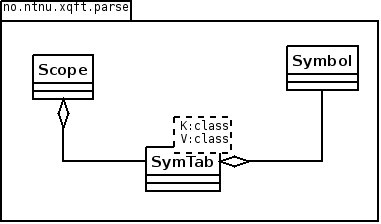
\includegraphics[scale=0.8]{img/uml1}
  \caption{Simplified UML overview of classes related to scope and symbol table}
\end{figure}

\section{Type checking}
XQuery/XPath has a well-defined type hierarchy:
\begin{figure}[!h]
  \centering
    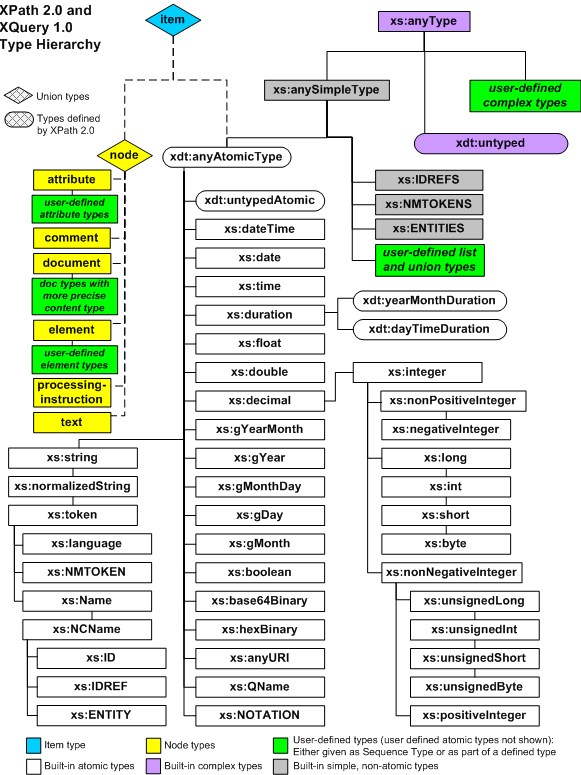
\includegraphics[scale=0.5]{img/xpathtypehierarchy}
  \caption{XQuery/XPath type hierarchy \cite{w3c04} (graphic copyright
  \copyright W3C)}
\end{figure}
All types are derived from the following types in the hierarchy:
\begin{itemize}
  \item Node types
  \item Structure types
  \item Atomic types
  \item Simple types
\end{itemize}


\chapter{Tainting Dependencies}
\label{sect:translation}
\label{chapter:translation}


One of the greatest challenges in translating XQuery to relational algebra, is
to translate the semantics of iterators. The iterative nature of expressions
such as \texttt{for} expressions and the bulk oriented relational processing
may seem contradictory. But because XQuery is a purely functional language, and
thus free of side effects, it is semantically sound to evaluate all iterations
of the iterator body in parallel.

In this chapter we will first present MarkXRemove. This was the first iterator translation proposal of this
project. As it had some flaws, the method was reinvented and evolved into Tainting Dependencies (TD), accomodating
for the deficiencies of MarkXRemove. The rest of the chapter is dedicated to this method. First some concepts will
be discussed, followed by methods for translating various features of XQuery into MQL relational algebra trees,
including the translation of iterators. Finally, the chapter will discuss some possible simplifications of trees
generated with TD.

\section{MarkXRemove}
\label{sect:translation:MarkXRemove}

Our original proposition to a method for translating XQuery ASTs into relational algebra was named MarkXRemove.
The rationale behind this name will be explained later. Eventhough it has many shortcomings and flaws, we
will in this section give a quick run through of the method. This is because when we in the next section present
``INSERTNAMEHERE'', which is an evolution and a refinement of MarkXRemove, the new method may be easier understood
when seen in the perspective of its origins. Another reason is that in case of further development of the
``INSERTNAMEHERE'', it may be of help to also know what will \textit{not} work, what will work partially and
\textit{why} it is flawed.

\subsection{Basics}
\label{sect:translation:mxr:basics}

The foundation of the method is that an iterator expression is always translated by calculating the cartesian
product of the iterator sequence and the iterator body, hence the ``X'' in the name. The ``remove'' stems from the
removing of tuples who ended up in the wrong iteration in the cross product result. The cartesian product and the
selection of tuples afterwards actually constitutes a kind of natural join (see section
\ref{sect:theory:relAlg:naturalJoin}) as we will see later.

As the translator comes across an iterator variable declaration, with the variable name $\chi$, it will augment
the representation of the iterator sequence belonging to this variable with an attribute $\chi$\textsf{numb}.
This new attribute will hold consecutive values from 1 to $n$ for a $n$ item long sequence, which will symbolise the
iteration number of the iterator expression seen isolated from possible other surrounding iterator expressions. A
function \texttt{counter()} returning the row number of a relation and a \texttt{project} operator will handle
the augmentation. The corresponding algebra tree is be stored in the symbol table. The ``mark'' of the name of the
method is because of this augmentation.

\subsection{FLWOR}
\label{sect:translation:mxr:flwor}
If the translator later comes accross a reference to an iterator variable $\chi$, it will get the tree from the
symbol table and return it to the referring node without any further ado. The translator is also required to know
which subtrees have a child that has referred to which iterator variable. This is because the $\chi$\textsf{numb}
column could be lost in a \texttt{project} operation without this knowledge.

When the translator returns to the iterator expression node for the variable $\chi$ after traversing the iterator
body, it will, as mentioned before, make sure that the cartesian product between the iterator sequence and body is
calculated. From the result of this, the tuples where the $\chi$\texttt{numb} stemming from the iterator
sequence does not line up with the $\chi$\texttt{numb} stemming from the body are removed. Any tuple with a
$\chi$\texttt{numb} value \texttt{NULL} will be kept.

A \texttt{NULL} value in attribute $\chi$\texttt{numb} for a tuple means that this tuple is not marked, i.e. it is
not dependant on which iteration the $\chi$ iterator expression is in. Unmarked tuples can e.g. stem
from the creation of a sequence. MarkXRemove translates sequence building such as \texttt{(}$e_{1}$\texttt{,
}$e_{1}$\texttt{)} to a simple disjoint union, $r(e_{1})\;\dot\cup\;r(e_{2})$. Where $r()$ symbolises a function
translating XQuery expressions into relational algebra.

The method creates quite simple algebra, as exemplified by the following query:
\begin{Verbatim}
for $i in (1,2,3) return 
  ($i, 'yes')
\end{Verbatim}

which is translated into this algebra:

\begin{Verbatim}
select(ifThenElse(isNull(value), true, eq(r.inumb,l.inumb))
  cross(
    project(inumb = counter(), value;
      make(name:=["value"], [1,2,3]))
    union(
      project(inumb = counter(), value;
        make(name:=["value"], [1,2,3]))
      make(name:=["value"], ['yes']))))
\end{Verbatim} 

\subsection{Flaws}
\label{sect:translation:mxr:flaws}
The main problem with MarkXRemove is its dependancy on particular ordering of tuples in a relation which is a
result of a cartesian product. Not only can not the \texttt{cross} operator promise the particular ordering of its
result, it can not promise any ordering at all. The ordering the method depends on is that for each tuple in the
left relation the tuple is repeated for all tuples in the right relation. This means that any item may apear
anywhere in the resulting sequence, which is not acceptable for evaluation of XQuery expressions where all
sequences are ordered.

Another problem with this method is that any sequence built which includes a reference to an iterator variable is
not fully calculated until the cartesian product between the corresponding relation and the variables iterator
sequence is evaluated. This makes it hard to evaluate expressions where such a sequence is a subexpression. The
iterator \textit{body} of this query:

\begin{Verbatim}
for $i (5,10) return
  ($i, 8) > (6,12)
\end{Verbatim}
would be translated into something like this relational algebra:
\begin{Verbatim}
project(value = gt(l.value, r.value), inumb
cross(
  union(
    project(inumb = counter(), value;
      make(name:=["value"], [5,10]))
    make(name:=["value"], [8]))
  make(name:=["value"], [3,12])))
\end{Verbatim}
which again would produce this relation:

\begin{figure*}[!h]
\centering
\begin{tabular}{|c|c|} \hline
$inumb$ & $value$ \\\hline
1 & \texttt{false} \\\hline
1 & \texttt{false} \\\hline
2 & \texttt{true} \\\hline
2 & \texttt{false} \\\hline
\texttt{NULL} & \texttt{true} \\\hline
\texttt{NULL} & \texttt{false} \\\hline
\end{tabular}
\end{figure*}

The query should of course be evaluated to $(true, true)$, as the \texttt{>} operator in XQuery yields $true$ if
\textit{one} item in the sequence on the left side of the operator is larger than \textit{one} item on the right.
This means that the relation would have to be pruned by a \texttt{select} or \texttt{group}, which can not be done
genericly in the relations current state. A possibility would be to postpone the pruning until after the relation
is crossed with the iterator sequence, but there would still not be any not-complex solution. This problem lead to
the introduction of variable dependancy tainting, as we will see in section \underline{\textbf{\LARGE
TODO:}}''omtainting''

\underline{\textbf{\LARGE TODO:}} her st\aa r det egentlig noe om numeric predicates, men det er kommentert bort. 
% Within the \texttt{scope} field of a relation returned from a \texttt{lookup} operator lies information about
% which child number the scope is relative to its sibling scopes. E.g. if a \texttt{lookup} had been executed on a
% index holding the following XML-document:
% \begin{Verbatim}
% <a>
%   <b>one</b>
%   <b>two</b>
% </a>
% \end{Verbatim}
% it would be possible to extract that the element containing ``two'' is the second \verb!<b>!-child of its parent.
% And its exactly this information MarkXRemove relies on when translating numeric predicate(see section
% \ref{sect:theory:xquery:Predicates}). But when a numeric predicate is applied to a step expression with a reverse
% axis, e.g. \texttt{ancestor::}, the numbering is reversed. This means that


\section{Inference Rule Language Explanation}
\label{sect:trans:TD:langExpl}
During this chapter we will present some inference rules. Table \ref{tab:trans:td:langExpl} explains some of the
the various typographical representations.

\begin{table}[h]
\centering
\begin{tabular}{l|l}

  $\longmapsto$  			& Translates into \\
  $\vartheta$ 				& A set of iterator dependencies \\
  \textsf{sans serif} 		& MQL expressions \\
  \texttt{monospaced} 		& XQuery expressions \\
  $e,\ldots,e_{n}$			& Generic expressions \\
  $\chi,\ldots,\chi_{n}$	& Generic variable names \\
  $I_{\chi}$				& The iterator expression which declares $\chi$ \\
  \textbf{bold} 			& Operations done during the generation of the algebra \\
  \textbf{r(}$e$\textbf{)} 	& Returns the relational algebraic representation of $e$   \\
  \textbf{t(}\textbf{r(}$e$\textbf{)}\textbf{,}$\vartheta'$\textbf{)} & Returns \textbf{r(}$e$\textbf{)} tainted
  with the dependencies $\vartheta'$ \\
  \textbf{B(r(}$e$\textbf{))} & Returns the effective boolean value of \textbf{r(}$e$\textbf{)}.
  
\end{tabular}
\caption{Explanation of inference rule symbols}
\label{tab:trans:td:langExpl}
\end{table}

Inference rules are generally in this format:
\begin{equation*}
\frac{condition}{e}\longmapsto \mbox{\textbf{r(}}e\mbox{\textbf{)}}
\end{equation*}

This should be read as: if condition $condition$ is satisfied, the XQuery expression $e$ will be translated into
\textbf{r(}$e$\textbf{)}.

Often MQL operator trees are depicted like this:
\begin{center}
\begin{tabular}{l}
\textsf{operator1(\ldots,l.attr, r.attr\ldots; } \\ \quad
\textsf{operator2(\ldots);} \\ \quad
\textsf{operator3(\ldots))}
\end{tabular}
\end{center}

This is to be interpreted as \textsf{operator2} is the left child of \textsf{operator1} and \textsf{operator3} is
the right child. MARS does not allow attribute names to contain punctuation marks or allow two attributes with the
same name within one relation. An operator combining two relations will therefore have renaming functionality. A
typical projection list of such an operator combining two relations which both contain the attribute $attr$ would
look something like: \textsf{\ldots rattr=right.attr, lattr=left.attr\ldots}. To make the inference rules
easier to read, this step has been dropped. The rules assume that the equal
named fields will automatically be given a prefix \textsf{l.} (left) or
\textsf{r.} (right) depending on which child the attribute stems from.

We assume the \textsf{union}-operator accepts relations with different schemas. The schema for the result
relation can be described as:
\begin{equation*}
schema(\textsf{union(}\alpha, \beta\texttt{)}) = schema(\alpha) \cup schema(\beta).
\end{equation*}

The tuples which have more fields in the result relation than they did in the relation they stem from will
have a \textit{NULL} value for the introduced attributes. It may be not be
desirable to implement the operator in such a way. In that case each
child-relation will have to be augmented with the attributes needed with an \textsf{project} operator.

\section{Basics}
\label{sect:trans:TD:basics}
The method assumes left-to-right traversal of the assymetric syntax tree. In most cases the traversal is
postorder, meaning a subtree can be evaluated independently from its ancestors -- the exception being the logical
context set by boolean operators. The relational algebra will thus be generated bottom-up. In addition to the
evaluated subtree, a node must be able to inform its parent node about its variable dependencies ($\vartheta$),
which we will discuss later.

One XQuery sequence is represented as one relation and one XQuery item is represented as one tuple. This is sound,
as all XQuery items are sequences, and all sequences are one-dimensional (section
\ref{sect:theory:xquery:basics}). As we mentioned in section \ref{sect:trans:MarkXRemove}, the MarkXRemove method
did actually not consider the ordering of items in sequences at all. In Tainting Dependencies, however, we have
introduced an attribute $index$ holding the intra sequence number of the item. Consider the XQuery sequence
\texttt{('a','b',}$\ldots$\texttt{,'z')}. With this attribute, the relational representation will be as follwing:

\begin{center}
\begin{tabular}{|c|c|} \hline
$index$ & $value$ \\\hline
1		& \texttt{'a'} \\\hline
2		& \texttt{'b'} \\\hline
$\ldots$& $\ldots$ \\\hline
$n$		& \texttt{'z'} \\\hline
\end{tabular}
\end{center}


As can be seen, the item value is stored in the $value$ attribute. For the course of this chapter we will, for the
sake of simplicity, treat $value$ as a polymorphic type attribute. This simplification has minimal consequences
for the method and the way XQuery expressions are translated. XQuery types and relational representation of such
will is handled in section \ref{sect:disc:typeSystem}.

Also for simplicity, the $index$, $documentId$, $pos$ and $scope$ attributes have sometimes been left out of the
fields specified in \textsf{project} operators. If the \textsf{project} operator is applied to the result of a
join or cartesian product, these fields will follow the $value$ attribute if nothing else is specified. That is, if
$r.value$ is projected, then so is $r.documentId$, etc\ldots if applicable.

Tainting Dependencies utilises a symbol table for storing of variables declared. The table has two functions:
\begin{itemize}
  \item \textbf{put(}$\chi$\textbf{, }\textbf{r(}$e$\textbf{))} -- will store the
  algebraic version of the expression bound to the variable \texttt{\$}$\chi$ with $\chi$ as the key.  
  \item \textbf{get(}$\chi$\textbf{)} -- will do a lookup in the table based on the name of the variable
  \texttt{\$}$\chi$ and return the algebraic version of the expression linked to it.
\end{itemize}
The symbol table handles scoping according to XQuery semantics (section \ref{sect:theory:xquery:Flwor}), meaning
the translator will always be able to find the right declared variable based on which node in the AST the
translator is visiting.

\subsection{Iterator Dependency Inheritance}
\label{sect:trans:TD:dependency}

The concept of iterator dependency form the basis of the Tainting Dependency method. Such dependency is
defined as follows:

\noindent
\begin{myDefinition}
An XQuery expression $e$ is \textbf{dependent} on an iterator $I_{\chi}$ if $e$
occurs within the iterator body of $I_{\chi}$ and if the evaluation of $e$ depends on the iteration number of $I_{\chi}$.
\label{def:iterVarDep}
\end{myDefinition}

An variable reference to an iterator variable \texttt{\$}$\chi$ is by this definition dependent on the iterator
$I_{\chi}$. Intuitively, an expression which subexpression is dependent on an iterator $I_{\chi}$ is also
dependent on this iterator -- we say the dependency is inherited. Consider the example subexpression of figure
\ref{fig:trans:td:varDep}, where \texttt{\$x} and \texttt{\$y} both are
iterator variables. Here, the expression $e_{1}$ is dependent on the two
iterators $I_{\mbox{\texttt{x}}}$ and $I_{\mbox{\texttt{y}}}$, while expression $e_{2}$ is only dependent on $I_{\mbox{\texttt{x}}}$.

\begin{figure}[h]
\centering
\tikzstyle{astNode}=[circle, draw=blue!70,fill=blue!20,solid,thick, minimum
size=26pt]
\begin{tikzpicture}[grow via three points={one child at (0,-1.5) and two
children at (-1.5,-1.0) and (1.5,-1.0)}]
\draw[loosely dotted, thick] (0,0) -- (0,-1);
\node at (0,-1) [astNode, label=above left:$e_{1}$ ] {\texttt{and}} 
child{node [astNode, label=above left:$e_{2}$] {\texttt{+}}
	child{node [astNode] {\texttt{\$x}}}
	child{node [astNode] {\texttt{3}}}
 }
child{node [astNode] {\texttt{\$y}}}
 ;
\end{tikzpicture}
\label{fig:trans:td:varDep}
\caption[Iterator variable dependency]{Iterator variable dependency}
\end{figure}

The iterator dependencies of an expression $e$ are part of the set $e.\vartheta$. As mentioned earlier,
an AST node must be able to inform its parent about the node's dependencies as well as the algebra generated. For
an expression $e$ this can be done by letting $e.\vartheta$ piggyback the \textbf{r(}$e$\textbf{)} returned. The
variable dependencies for an expression $e$ with the subexpressions $e_{1},\ldots,e_{n}$ can be described as
following:
\begin{equation}
e.\vartheta = e_{1}.\vartheta\cup\ldots\cup e_{n}.\vartheta
\label{eq:trans:TD:depInheritance}
\end{equation}

The dependency on the iterator $I_{\chi}$ manifest itself relationally by the
attribute $\chi$$numb$. The value of $\chi$$numb$ is the iteration number of $I_{\chi}$, that is, for a tuple ($\chi$$numb$, $value$) the value $value$
will appear in the $\chi$$numb$th iteration of $I_{\chi}$.

When an iterator variable \texttt{\$}$\chi$ is declared it is assigned a $\chi$$numb$ by renaming the $index$
field of the corresponding iterator sequence $\chi$$numb$. Which leads us to the inference rule for translating the
(optional) \texttt{for} clause of a FLWOR expression:
\begin{equation}
\frac{}{\mbox{\texttt{for \$}}\chi \mbox{\texttt{ in }} e \mbox{\texttt{\ldots}}}\longmapsto
\begin{array}{l}
\mbox{\textbf{put(}}\chi\mbox{\textbf{, }} \\ \quad
\mbox{\textsf{project(}}\chi\mbox{\textsf{numb = index, index=1, value;}} \\ \quad \quad
\mbox{\textbf{r(}}e\mbox{\textbf{)}\textsf{)}\textbf{)}}
\end{array}
\label{rule:trans:TD:forbind}
\end{equation}
Where the dependencies piggybacking the \textsf{project} operator can be
expressed as: $\vartheta = e.\vartheta \cup \chi$.

For a \texttt{for} clause with multiple variable bindings the rule must be applied once per binding as if there
is one FLWOR expression per binding, and the $n$th binding is a FLWOR expression in the $(n-1)$th bindings
return clause. This is in accordance with the XQuery semantics, and is one of
the rewrite rules into XQuery Core (see section \ref{sect:theory:xquery:XQcore}).

From definition \ref{def:iterVarDep} it can be seen that $\chi$ is not part of
the set of dependencies the iterator $I_{\chi}$ returns its parent. This is in
fact the only case where a variable is removed from a dependency set. Because of
this, we must be careful not to incidentally remove a $\chi$$numb$ attribute
from a relation by means of a \textsf{project} operator.

When we in this chapter write $\vartheta$ enclosed in MQL syntax it is to be
interpreted as a comma separated list of all the attributes linked to the
dependencies in the set $\vartheta$. As an example, the dependency set
$\vartheta = \left\{\mbox{\texttt{x}},\mbox{\texttt{y}},\mbox{\texttt{z}}\right\}$, is read as \textsf{xnumb, ynumb, znumb} in an MQL environment.

XQuery variable reference expressions, be it iterator, \texttt{let} or \texttt{declare} variables, are translated
to relational algebra quite simply by fetching the tree linked to the variable name in the symbol table:
\begin{equation}
\frac{}{\mbox{\texttt{\$}}\chi}\longmapsto
\mbox{\textbf{get(}}\chi\mbox{\textbf{)}}
\label{rule:trans:TD:varRef}
\end{equation}


\subsection{Iterator Dependency Tainting}
\label{sect:trans:TD:tainting}

The iterator body of an iterator with a iterator sequence with length $n$ will
have to be executed $n$ times. This can be done by e.g. evaluating the cartesian
product between the body or the sequence, as with the MarkXRemove method. To
avoid any denormalised intermediate results, an ideal solution would be to
always calculate such products after all other evaluations of the query is
done. Consider the following simple example of the query $e$:

\begin{center}
\begin{tabular}{l}
\texttt{for \$a in (1, 2) return} \\ \qquad
\texttt{for \$b in (3, 4) return} \\ \qquad \qquad
\texttt{5 + 6}
\end{tabular}
\end{center}

For this query the result can be calculated like this:
\noindent
\begin{center}
\textbf{r(}$e$\textbf{)}$=$\textbf{r(}\texttt{(1, 2)}\textbf{)}$\times$\textbf{r(}\texttt{(3,
4)}\textbf{)}$\times$\textbf{r(}\texttt{5 + 6}\textbf{)}.
\end{center}
\noindent

But such a simple solution is not adequate if there is a reference to an iterator variable somewhere within the
iterator body. This was managed by MarkXRemove by implementing inheritance of iterator dependencies, similar to
the concept discussed in section \ref{sect:trans:TD:dependency}, and replacing the cartesian product operator with
something like a natural join operator (section \ref{sect:trans:mxr:basics}).

MarkXRemove has shortcomings when it comes to evaluating expressions where a
sequence constructed with at least one iterator dependent expression is a subexpression. Tainting Dependencies mend for this by requiring that
all items constituting the result of an iterator dependent expression are
iterator dependent. To meet this requirement, dependency tainting is
introduced.

\noindent
\begin{myDefinition}
Iterator dependency \textbf{Tainting} is to impose a representation of one expression for each iteration of the
iterators another expression is dependent on.
\end{myDefinition}

During sequence construction, expressions explicitly taint all other expressions part of the construction with
their dependencies. Consider this subexpression:
\begin{center}
\begin{tabular}{l}
\quad \;\, $\vdots$  \\
\texttt{(}$e_{1}$\texttt{, }$e_{2}$\texttt{)}\\
\quad \;\, $\vdots$  
\end{tabular}
\end{center}
Where $e_{1}.\vartheta = \left\{\chi_{1}\right\}$ and $e_{2}.\vartheta = \emptyset$. Here $e_{2}$ will be tainted
by $e_{1}$'s dependency on $\chi_{1}$, but as $e_{2}$ have no dependencies, $e_{1}$ will not be tainted. The
tainting process is carried out by calculating the cartesian product of $e_{2}$ and the $\chi_{1}$$numb$ column of
\texttt{\$}$\chi_{1}$ stored in the symbol table.

More generally, for a sequence constructing expression $e$, \texttt{(}$e_{1}$\texttt{, \ldots, }$e_{n}$\texttt{)},
tainting of an subexpression $e_{i}$ can be expressed like this: 
\begin{center}
\begin{equation}
\begin{array}{l}
e.\vartheta = e_{1}.\vartheta \cup \ldots \cup e_{n}.\vartheta = \left\{\chi_{1},\ldots\chi_{m}\right\} \\
i \in \left\{1,\ldots,n\right\} \\
\mbox{\textbf{t(r(}}e_{i}\mbox{\textbf{),}}e.\vartheta\mbox{\textbf{)}} = 
\mbox{\textbf{r(}}e_{i}\mbox{\textbf{)}} \times {\displaystyle \prod_{\chi_{j} \in (e.\vartheta -
e_{i}.\vartheta)}} \mbox{\textsf{project(}}\chi_{j}numb\mbox{\textsf{;
}\textbf{get(}}\chi_{j}\mbox{\textbf{)}\textsf{)}}
\end{array}
\label{eq:trans:TD:taint}
\end{equation}
\end{center}

\subsection{Unique Iterations}
\label{sect:trans:TD:implic}
Consider an XQuery expression consisting of nested iterators $I_{\chi_1},\ldots,I_{\chi_n}$, where $I_{\chi_j}$
($1<j<n$) occurs within the iterator body of $I_{\chi_{j-1}}$. As per XQuery semantics, the iterator body of a
iterator $I_{\chi_j}$ is evaluated once for each of the items in the iterator sequence of $I_{\chi_j}$. And because
of the nesting, $I_{\chi_j}$ will have to be evaluated once per item in the iterator sequence of $I_{\chi_{j-1}}$.
The consequence of this is that the number of unique iterations the body of $I_{\chi_j}$ is actually evaluated can
be expressed like this: 
\begin{equation*}
\mbox{\textit{unique iterations evaluated for body of}}I_{\chi_j}=\displaystyle \prod_{i=1}^{j}card(I_{\chi_i})
\end{equation*}  
Where $card(I_{\chi})$ is a function returning the cardinality of the iterator sequence of $I_{\chi}$.

Of these nested iterators, a subexpression $e$ is dependent on the subset
$\left\{I_{\chi_k},I_{\chi_l}\right\}$. Because of dependency tainting and inheritance, the relational
depiction of $e$ will have a representation in all possible iteration
combinations of $I_{\chi_k}$ and $I_{\chi_l}$. A tuple in $e$, ($index, \chi_k{numb},\chi_l{numb}, value$), represents one of these unique
iterations. When $I_{\chi_k}$ is in its $\chi_k{numb}$th iteration and $I_{\chi_l}$ is in its $\chi_l{numb}$th
iteration, the item in position $index$ of the sequence returned from $e$ will be $value$. Let $I_{\chi_m}$ also
be one of the nested iterators, but one which $e$ is not dependent on. $e$ will evaluate to the same result
regardless of which iteration $I_{\chi_m}$ is in given the iteration number of
$I_{\chi_k}$ and $I_{\chi_l}$ is the same.

When an subexpression such as $e$ is used in further evaluation, it is important to seperate these iterations from
each other. This is done by grouping the relation on all unique combinations of its iterator dependency attributes.
Grouping can be done either by the \textsf{group} operator or by specifying the attributes to group by in the
partition list of the \textsf{numberate} operator.

Often the evaluation of an expression use the values of each of its
subexpressions. E.g. an addition expression is evaluated by adding the value of its first subexpression with the value of the second. To be able to calculate
such expressions, the values of the subexpressions will have to be in the same relation. This can be achieved by
evaluating the cartesian product of the subexpressions. Assumed that the subexpressions are independent of
iterators or are not dependent on the same iterators this is sufficient. But if they are depentent on one or more
iterators in common, the result of the cartesian product will have to be synchronised on the common iterators
iterations. This allows evaluation in each unique iteration, and is solved by turning the cartesian product into
an equi-join.

Generally, for such an expression $e$, with the subexpressions $e_1$ and $e_2$ this can be written
like this:
\begin{equation*}
\mbox{\textbf{r(}}e\mbox{\textbf{)}}=
\begin{array}{l}
\mbox{\texttt{\ldots}} \\
\mbox{\textsf{hhjoin([}}(e_1.\vartheta\cap e_2.\vartheta)\mbox{\textsf{], [}}(e_2.\vartheta\cap e_1.\vartheta)
\mbox{\textsf{]\ldots}} \\ \quad
\mbox{\textbf{r(}}e_1\mbox{\textbf{)}} \\ \quad
\mbox{\textbf{r(}}e_2\mbox{\textbf{)}\textsf{)}}
\end{array}
\end{equation*}

The dependencies $e.\vartheta$ is described by equation \ref{eq:trans:TD:depInheritance}. If $e_{1}.\vartheta \neq
e_{2}.\vartheta$ each subexpression will be implicitly tainted by the other's unique dependencies.

How the effective boolean function \textbf{B(r(}$e$\textbf{))} works will be discussed in section
\ref{sect:disc:effBool}. In this chapter is sufficient to consider it as a grouping operator, grouping on the
attributes specified by $e.\vartheta$ (i.e. all known unique iterations). For each group it will produce a field
$pred$ representing the effective boolean value of $e$ in that unique iteration. If $e$ holds a singleton numeric
value in one group $pred$ will hold this value, in all other cases it will hold a boolean value. The result
relation of the function will in addition to the $pred$-attribute contain all the attributes implied by
$e.\vartheta$. The main reason this function is introduced at all is that it ensures that a incoming relation
will have \emph{exactly one} tuple per unique iteration.

\subsection{Literals}
\label{sect:trans:TD:literal}

The XQuery Full Text specification\cite{w3c01} defines a number of literals as seen in figure
\ref{fig:trans:TD:litEBNF}. A \texttt{StringLiteral} is a text string enclosed in apostrophes or quotation marks,
and the numeric literals are similar to numeric types from other programming languages. 

\begin{figure}[h]
\begin{Verbatim}
[85] Literal        ::= NumericLiteral|StringLiteral
[86] NumericLiteral ::= IntegerLiteral|DecimalLiteral|DoubleLiteral
\end{Verbatim}
\caption[Literals in XQuery]{Definition of literals in XQuery Full Text}
\label{fig:trans:TD:litEBNF}
\end{figure}

To be able to include such expressions in evaluation of relational algebra, they need a relational representation.
As we in this chapter assume $value$ is a polymorphic type attribute, with the help of the \textsf{make} operator
translation of literals is done in the following way:

\begin{equation}
\frac{e \in \left\{Literals\right\}}{e}\longmapsto
\mbox{\textsf{make(name:=["index","value"], [1, }}e\mbox{\textsf{])}}
\label{rule:trans:TD:literal}
\end{equation}

This is a general way to translate literals, but there exists quite a few simplifications. Most importantly when
constructing sequences entirely composed of literals, as we will discuss in section
\ref{sect:trans:TD:simplifications}.


\section{Sequence Construction}
\label{sect:trans:TD:seqBuild}

A sequence in XQuery can be built with the comma operator(\texttt{,}). But this operator is the XQuery operator
with the lowest precedence, therefore, in most cases a sequence construction expression will be enclosed in
paratheses. This is to solve parser ambiguities, which can be seen in the excerpt of the W3C XQuery EBNF
specification\cite{w3c00} in figure \ref{fig:trans:TD:seqEBNF}. An \texttt{ExprSingle} can solely consist of a
\texttt{ParenthesizedExpr} via a series of productions omitted from the figure. Also note a \texttt{ExprSingle}
can be a \texttt{FLWORExpr}.

\begin{figure}[h]
\begin{Verbatim}
[33] FLWORExpr         ::= (ForClause | LetClause)+ WhereClause? 
                               OrderByClause? "return" ExprSingle
[45] IfExpr            ::= "if" "(" Expr ")" "then" ExprSingle 
                               "else" ExprSingle
[31] Expr              ::= ExprSingle ("," ExprSingle)*
[89] ParenthesizedExpr ::= "(" Expr? ")"
\end{Verbatim}
\caption[Excerpt from W3C XQuery EBNF]{Excerpt from W3C XQuery EBNF showing
sequence construction}
\label{fig:trans:TD:seqEBNF}
\end{figure}

As also can be seen from the figure the \texttt{return}-clause of a FLWOR expression, as many other expressions,
accepts an \texttt{ExprSingle}. If a sequence is to be constructed in the \texttt{return}-clause, it will have to
be parenthesised.

With the concept of tainting and iterator dependencies explained, we are now ready to introduce the translation of
an XQuery sequence construction expression:

\begin{equation}
\frac{}{e_{1}\mbox{\texttt{, \ldots, }}e_{n}}\longmapsto
\begin{array}{l}
\mbox{\textsf{numberate(index, [sprIdx, index], [}}\vartheta\mbox{\textsf{];}} \\ \quad
\mbox{\textsf{union(}} \\ \quad \quad
\mbox{\textsf{project(sprIdx=1, index, value; }} \\ \quad \quad \quad
\mbox{\textbf{t(r(}}e_{1}\mbox{\textbf{), }}\vartheta\mbox{\textbf{)}\textsf{);}} \\ \quad \quad
\qquad\vdots\\ \quad \quad
\mbox{\textsf{project(sprIdx=}\textit{n}\textsf{, index, value; }} \\ \quad \quad \quad
\mbox{\textbf{t(r(}}e_{n}\mbox{\textbf{), }}\vartheta\mbox{\textbf{)}\textsf{)))}}
\end{array}
\label{rule:trans:TD:seqConstr}
\end{equation}

Where $\vartheta=e_{1}.\vartheta \cup \ldots \cup e_{n}.\vartheta$. Notice how all subexpressions are tainted with
the iterator dependencies of all the others.

The basis of a sequence construction is the \textsf{union} operator -- as with MarkXRemove. But because we in
Tainting Dependencies have introduced the explicit ordering of items with the
$index$ attribute, additional operators have been added. Each item in the sequences returned from the subexpressions is equipped with a
temporary field $sprIdx$ (superindex) holding the relative position of each subexpression. Based on the
positioning defined by $sprIdx$ and $index$ the \textsf{numberate} operator can renumberate the resulting
sequence. The numbering must partition on the fields corresponding to the dependencies in $\vartheta$, to separate
the different sequences constructed for all known unique iterations.

\begin{myExample}
\label{ex:trans:TD:simpleSeq}
\begin{figure}[h]
\begin{equation*}
\begin{array}{l}
\mbox{\texttt{for \$a in (10,20) return}} \\ \quad 
\underbrace{ \mbox{\texttt{(\$a, "no")}} }_{e_{1}}
\end{array}
\end{equation*}
\caption{Simple XQuery query}
\label{fig:trans:TD:simpQuery}
\end{figure}
Consider the simple XQuery query of figure \ref{fig:trans:TD:simpQuery}. Here \textbf{r(}\texttt{\$a}\textbf{)}
will taint \textbf{r(}\texttt{"no"}\textbf{)} with its dependency on the iterator $I_{\mbox{\texttt{a}}}$, the
result of which is shown in figure \ref{fig:trans:TD:simpl:ryes}. Further, we can see that for each iteration of
$I_{\mbox{\texttt{a}}}$ the \texttt{return}-clause will return a sequence of two items. Having in mind that
$anumb$ ($anb$ in figure) holds the iteration number of $I_{\mbox{\texttt{a}}}$, this can be seen in figure
\ref{fig:trans:TD:simpl:rall}.

\begin{figure}[!h]
\centering
\subfigure[\textbf{r(}\texttt{\$a}\textbf{)}]{
\begin{tabular}{|c|c|c|} \hline
$anb$ & $idx$ & $val$ \\ \hline
1 & 1 & 10 \\ \hline
2 & 1 & 20 \\ \hline
\end{tabular}
\label{fig:trans:TD:simpl:ra}
}
\qquad
\subfigure[\textbf{t(r(}\texttt{"no"}\textbf{),}\textbf{r(}\texttt{\$a}\textbf{)}$.\vartheta$\textbf{)}]{
\begin{tabular}{|c|c|c|} \hline
$anb$ & $idx$ & $val$ \\ \hline
1 & 1 & \texttt{"no"} \\ \hline
2 & 1 & \texttt{"no"} \\ \hline
\end{tabular}
\label{fig:trans:TD:simpl:ryes}
}
\qquad
\subfigure[\textbf{r(}\texttt{(\$a, "no")}\textbf{)}]{
\begin{tabular}{|c|c|c|} \hline
$anb$ & $idx$ & $val$ \\ \hline
1 & 1 & 10 \\ \hline
2 & 1 & 20 \\ \hline
1 & 2 & \texttt{"no"} \\ \hline
2 & 2 & \texttt{"no"} \\ \hline
\end{tabular}
\label{fig:trans:TD:simpl:rall}
}

\caption[Example: constructing a sequence]{Applying translation rule \ref{rule:trans:TD:seqConstr} on (a) and (b)
yields (c). Attribute names are shortened \label{fig:trans:TD:simpleSeq}}
\end{figure}

The sequence construction rule also holds even if the subexpressions of the
soon-to-be sequence are within the body of an iterator the sequence is not
dependent on. Expanding the query of figure \ref{fig:trans:TD:simpQuery} we get
the query of figure \ref{fig:trans:TD:expandQuery}. 

\begin{figure}[h]
\begin{equation*}
\begin{array}{l}
\mbox{\texttt{for \$a in (10,20) return}} \\ \quad
\mbox{\texttt{for \$b in (50,75) return}} \\ \quad \quad
\underbrace{ \mbox{\texttt{(\$a, "no")}} }_{e_{1}}
\end{array}
\end{equation*}
\caption{Query of figure \ref{fig:trans:TD:simpQuery} expanded}
\label{fig:trans:TD:expandQuery}
\end{figure}

In this query, notice the innermost \texttt{return}-clause expression, $e_{1}$, is identical to $e_{1}$ in the
previous query. Here, the result of the sequence construction will still be the relation shown in figure
\ref{fig:trans:TD:simpl:rall}, because $e_{1}.\vartheta=\left\{I_{\mbox{\texttt{a}}}\right\}$ -- also as before.
$e_{1}$ is not aware of the iterator $I_{\mbox{\texttt{b}}}$ -- and does not need to be either, as the result of
$e_{1}$ is independent of which iteration number $I_{b}$ is in.

\end{myExample}

\subsection{FLWOR Expressions}
\label{sect:trans:TD:simpleFLWOR}
The \texttt{let} clause does not explicitly cause any dependencies, only variable binding, and can therefore be
translated into storing the algebraic version of the expression to be bound in the symbol table:
\begin{equation}
\frac{}{\mbox{\texttt{let \$}}\chi \mbox{\texttt{ := }}e \mbox{\texttt{ \ldots}}}\longmapsto
\mbox{\textbf{put(}}\chi\mbox{\textbf{, r(}}e\mbox{\textbf{))}}
\label{rule:trans:TD:letbind}
\end{equation}
The iterator dependences $e.\vartheta$ is stored along with \textbf{r(}$e$\textbf{)} and will piggyback this
algebra tree if it later fetched from the symbol table. If there is more than one variable binding in the
\texttt{let} clause the rule must be applied once per binding as if one binding were one \texttt{let} clause.

As seen by the exerpt of the W3C XQuery EBNF specification in figure \ref{fig:trans:TD:seqEBNF}, a FLWOR
expression may be structured in infinitely many ways. For simplicity and readablilty the translation of such
expressions will be split up in more managable pieces. 

A FLWOR expression may have multiple \texttt{for} clauses, and a \texttt{for} clause may have multiple iterator
variable bindings. This means that one FLWOR may consist of many iterators, the semanics of which is described in
section \ref{sect:method:ast_rewrite}. We assume all possible iterator dependencies generated from the FLWOR, that
is, all iterator variables bound, is stored in a ordered set $\beta$. The dependencies are ordered in the order of
which the corresponding iterator variables are bound, i.e. top down, left to right while parsing the query. When
enclosed in MQL syntax $\beta$ is, as $\vartheta$, to be read as a comma seperated list of the attributes
corresponding to the dependencies.

\begin{figure}[h]
\centering
\begin{tabular}{l}
$[$\texttt{for}/\texttt{let \ldots}$]+$ \\ \quad
$[$\texttt{where }$e_2]?$ \\ \quad
$[$\texttt{order by }$e_3]?$ \\
\texttt{return }$e_4$
\end{tabular}
\label{fig:trans:TD:flworIll}
\caption{Illustration of a FLWOR expression}
\end{figure}

The translation of a single FLWOR like the one illustrated in figure \ref{fig:trans:TD:flworIll} will be executed
as shown in figure \ref{fig:trans:TD:flworExecute}. Firstly, all \texttt{for} and \texttt{let} variables will be
bound as described by the rules \ref{rule:trans:TD:forbind} and \ref{rule:trans:TD:letbind}, respectively.
Further, the \texttt{return} clause will be evaluated. If there is a \texttt{where} clause present, it is
evaluated next, based on the \texttt{where} expression and the result of the \texttt{return} clause, referred to as
\textbf{r(}$e_{C}$\textbf{)}. The order of the items returned from the FLWOR is conditioned by the presens of an
\texttt{order by} clause in the expression. If there is a \texttt{order by} clause, it will order the intermediate
result from the \texttt{return} or \texttt{while} clause, and finalise the FLWOR. If there is no \texttt{order by}
clause, the final evaluation of the FLWOR will be to order the intermediate result according to the iterators.

\begin{figure}[h]
\centering

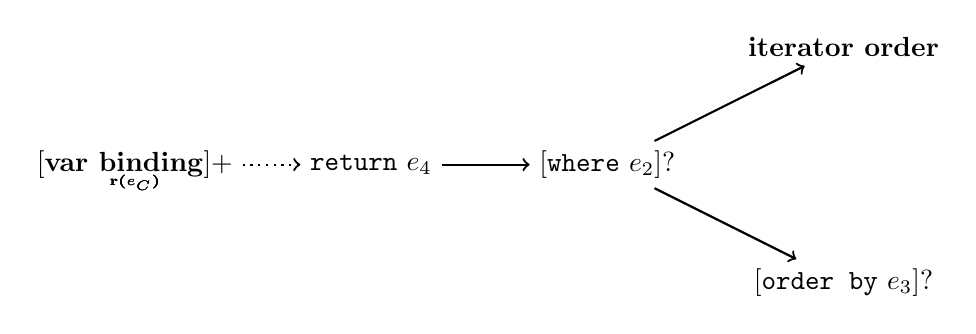
\begin{tikzpicture}

\node (bind) at (0,0) {$[$\textbf{var binding}$]+$};
\node (return) at (3,0) {\texttt{return} $e_{4}$};
\node (where) at (6,0) {$[$\texttt{where} $e_{2}]?$};
\node (itord) at (9,1.5) {\textbf{iterator order}};
\node (ordby) at (9,-1.5) {$[$\texttt{order by} $e_{3}]?$};
\draw [->,dotted,thick] (bind) to (return);
\draw [->,thick] (return) to (where) node[below,midway] {\tiny\textbf{r(}$e_{C}$\textbf{)}};
\draw [->,thick] (where) to (itord) node[below,midway] {\tiny\textbf{r(}$e_{C}$\textbf{)}};
\draw [->,thick] (where) to (ordby) node[below,midway] {\tiny\textbf{r(}$e_{C}$\textbf{)}};
\end{tikzpicture}
\label{fig:trans:TD:flworExecute}
\caption[FLWOR translation order]{Illustration of step-by-step translation of FLWOR.}
\end{figure}



Any possible iteration, ordering og filtering will be handled by other clauses than the \texttt{return} clause.
The \texttt{return} clause will just ship the evaluated version of the \texttt{return} expression forward:
\begin{equation}
\frac{}{\mbox{\texttt{return }}e_{4}}\longmapsto
\mbox{\textbf{r(}}e_{4}\mbox{\textbf{)}}
\label{rule:trans:TD:returnTaint}
\end{equation}


\subsubsection{Iterator Ordering}
The \texttt{return} clause is evaluated once for iteration for each of the iterators of the FLWOR expression. The
results of these evaluations are concatenated to form the result of the FLWOR expression. If the \texttt{return}
expression is not dependent on a iterator, its relational form will not have a representation for each
of the iterators iterations and will have to be tainted.

Because each FLWOR iterator creates a new sequence, renumbering is needed. No expression in a sibling or parent
scope of the iterator $I_{\chi}$ may be dependent on $I_{\chi}$. Thus, $\chi$ is not part of the dependencies
$I_{\chi}.\vartheta$ returned from the iterator, and the corresponding $\chi{numb}$ attribute must be removed. 

For each allready bound iterator variable $\chi$, from right to left, bound in an \texttt{for} clause,
the following translation is applied:
\begin{equation}
\frac{}{\mbox{\textbf{iterator order}}}
\longmapsto
\begin{array}{l}
\mbox{\textsf{numberate(index, [}}\beta\mbox{\textsf{, index], [}}\vartheta\mbox{\textsf{];}} \\ \quad
\mbox{\textbf{t(r(}}e_{C}\mbox{\textbf{), }}\beta\mbox{\textbf{)}}
\end{array}
\label{rule:trans:TD:itOrd}
\end{equation}

Where $\vartheta = e_{C}.\vartheta - \chi$.

From equation \ref{eq:trans:TD:taint} it is clear that a expression allready dependent on any iterator in
$\beta$ will not be re-tainted by these iterators.

The \textsf{numberate} operator will have to partition on the remaining dependencies in $\vartheta$ to seperate
the sequences returned from the iterator for all iterators the result is dependent on, as described in section
\ref{sect:trans:TD:implic}.

\begin{myExample}
Consider the query of figure \ref{fig:trans:TD:dblFor}. Notice the expression in the \texttt{return} clause ($e_1$)
is the same as $e_1$ in example \ref{ex:trans:TD:simpleSeq}.

\begin{figure}[h]
\begin{equation*}
\begin{array}{l}
\mbox{\texttt{for \$a in (10,20),}} \\
\mbox{\texttt{\phantom{abcd}\$b in (50,75)}} \\ 
\mbox{\texttt{return }}\underbrace{\mbox{\texttt{(\$a, "no")}} }_{e_{1}}
\end{array}
\end{equation*}
\caption{Example query with two iterators.}
\label{fig:trans:TD:dblFor}
\end{figure}

Expression $e_{1}$ is not depentant on $I_{\mbox{\texttt{b}}}$, and by rule \ref{rule:trans:TD:itOrd} will be
tainted by this iterator. The result of the tainting is shown in figure \ref{fig:trans:TD:final:taint}. The
expression will however not be tainted by $I_{\mbox{\texttt{a}}}$, as it is allready dependent on this iterator
(ref. equation \ref{eq:trans:TD:taint}).

\begin{figure}[h]
\centering
\subfigure[\textbf{t(r(}$e_{1}$\textbf{), \{}\texttt{b}\textbf{\})}]{
\begin{tabular}{|c|c|c|c|} \hline
$bnumb$ & $anumb$ & $index$ & $value$ \\ \hline
1 & 1 & 1 & 10 \\ \hline
1 & 2 & 1 & 20 \\ \hline
1 & 1 & 2 & \texttt{"no"} \\ \hline
1 & 2 & 2 & \texttt{"no"} \\ \hline
2 & 1 & 1 & 10 \\ \hline
2 & 2 & 1 & 20 \\ \hline
2 & 1 & 2 & \texttt{"no"} \\ \hline
2 & 2 & 2 & \texttt{"no"} \\ \hline
\end{tabular}
\label{fig:trans:TD:final:taint}
}
\qquad
\subfigure[\textbf{r(}$I_{\mbox{\texttt{a}}}$\textbf{)}]{
\begin{tabular}{|c|c|} \hline
$index$ & $value$ \\ \hline
1 & 10 \\ \hline
2 & \texttt{"no"} \\ \hline
3 & 10 \\ \hline
4 & \texttt{"no"} \\ \hline
5 & 20 \\ \hline
6 & \texttt{"no"} \\ \hline
7 & 20 \\ \hline
8 & \texttt{"no"} \\ \hline
\end{tabular}
\label{fig:trans:TD:final:rIa}
}
\caption[Example: resolving simple FLWOR]{Evaluating the query in figure \ref{fig:trans:TD:dblFor} yields the
intermediate result (a) and the final result (b).\label{fig:trans:TD:finalizeExp}}
\end{figure}

With the expression tainted with all possible iterator dependencies of the FLWOR, renumbering is the last
operation required to resolve the query. The \textsf{numberate} operator will sort the tuples first on $anumb$,
then on $bnumb$ and finally $index$ before numbering. As the FLWOR itself does not have any dependencies the
numeration will not be grouped on any attributes. The result of the query is shown in figure
\ref{fig:trans:TD:final:rIa}.
\end{myExample}

\subsubsection{Where Clause}
The W3C describes the FLWOR expression as generating a tuple stream which contains one tuple for each combination
of values bound in the expression\cite{w3c00}. In this view, the optional \texttt{where} clause serves a filter for
these tuples. The expression in the \texttt{where} clause is evaluated once for tuple. If the boolean value of this
expression is $true$, the tuple is retained, if the boolean value is $false$ the tuple is discarded.

The \texttt{where} clause can be evaluated by only selecting the iteration combinations where the \texttt{where}
expression is true. The result of this will be joined with the result of the \texttt{return} clause. If the result
from the \texttt{return} clause and the \texttt{where} expression has no common iterator dependencies, the
equi-join will have to be replaced by a cartesian product, as discussed in \ref{sect:trans:TD:implic}.

\begin{equation}
\frac{}{\mbox{\texttt{where }}e_2}\longmapsto
\begin{array}{l}
\mbox{\textsf{hhjoin([l.}}(e_{C}.\vartheta \cap e_2.\vartheta)\mbox{\textsf{], [r.}}(e_{2}.\vartheta \cap
e_{C}.\vartheta)\mbox{\textsf{], [l.value, }} \vartheta\mbox{\textsf{];}} \\ \quad
\mbox{\textbf{r(}}e_{C}\mbox{\textbf{)\textsf{;}}} \\ \quad
\mbox{\textsf{select(xqBoolean(value);}} \\ \quad \quad
\mbox{\textbf{r(}}e_{2}\mbox{\textbf{)}\textsf{))}}
\end{array}
\label{rule:trans:TD:where}
\end{equation}

Where $\vartheta = e_{C} \cup e_{2}$, and \textbf{r(}$e_{C}$\textbf{)} is the result of the translation done in
the \texttt{return} clause.

\textsf{l.}$(e_{C}.\vartheta \cap e_2.\vartheta)$ is short for
\textsf{l.}$\chi_1$\textsf{numb,\ldots,l.}$\chi_n$\textsf{numb}, where $e_{C}.\vartheta \cap e_2.\vartheta =
\left\{\chi_1,\ldots,\chi_n\right\}$.

By employing the \textsf{select} operator before the joining of the two relations the number of tuples needed to
be read to execute the join will be minimized. Further, as the \textsf{hhjoin} operator allows for declaring which
attributes to be projected, there is no need for a seperate \textsf{project} operator.

\begin{myExample}
Consider the XQuery query of figure \ref{fig:trans:TD:whereQuery}. The evaluation of $e_{1}$ is very similar to
the evaluation of $e_{1}$ of example \ref{ex:trans:TD:simpleSeq}, and the is shown in figure
\ref{fig:trans:TD:where:re1}. The \texttt{where} clause contains a comparison expression, which will be discussed
later. Figure \ref{fig:trans:TD:where:whereE} shows the result relation of the \texttt{where} expression.

\begin{figure}[h]
\centering
\begin{equation*}
\begin{array}{l}
\mbox{\texttt{for \$a in (10,20)}} \\
\mbox{\texttt{where \$a > 15}} \\
\mbox{\texttt{return}} \underbrace{\mbox{\texttt{(\$a, 14)}}}_{e_{1}}
\end{array}
\end{equation*}
\caption{A FLWOR expression with a \texttt{where} clause \label{fig:trans:TD:whereQuery}}
\end{figure}

\begin{figure}[h]
\centering
\subfigure[\textbf{r(}$e_{1}$\textbf{)}]{
\begin{tabular}{|c|c|c|} \hline
$anb$ & $idx$ & $val$ \\ \hline
1 & 1 & 10 \\ \hline
1 & 2 & 14  \\ \hline
2 & 1 & 20 \\ \hline
2 & 2 & 14  \\ \hline
\end{tabular}
\label{fig:trans:TD:where:re1}
}
\qquad
\subfigure[\textbf{r(}\texttt{\$a > 15}\textbf{)}]{
\begin{tabular}{|c|c|c|} \hline
$anb$ & $idx$ & $val$ \\ \hline
1 & 1 & $false$ \\ \hline
2 & 1 & $true$ \\ \hline
\end{tabular}
\label{fig:trans:TD:where:whereE}
}
\qquad
\subfigure[]{
\begin{tabular}{|c|c|c|} \hline
$anb$ & $idx$ & $val$ \\ \hline
2 & 1 & 20 \\ \hline
2 & 2 & 14  \\ \hline
\end{tabular}
\label{fig:trans:TD:where:intr}
}

\caption[Example: Evaluation of where clause]{Applying rule \ref{rule:trans:TD:where} on (a) and (b)
yields (c). Attribute names are shortened. \label{fig:trans:TD:whereClause}}
\end{figure}

During the evaluation of the FLWOR, the tuples in the \texttt{where} expression relation where $value$ ($val$ in
figure) is not $true$ will be removed. The result is a relation with a single tuple where $anumb$ holds the value
$2$. This result is then joined with the $e_1$ relation on $anumb$, as shown in figure
\ref{fig:trans:TD:where:intr}. Rule \ref{rule:trans:TD:itOrd} will have to be applied to complete the
evaluation of the query.
\end{myExample}


\subsubsection{Order By Clause Ordering}

As can be seen in figure \ref{fig:trans:TD:ordEBNF}, an \texttt{Order by} clause may contain several specifications on
how to order and what to order by.
\begin{figure}[h]
\begin{Verbatim}
[38] OrderByClause ::= (("order" "by") | ("stable" "order" "by")) 
                           OrderSpecList
[39] OrderSpecList ::= OrderSpec ("," OrderSpec)*
[40] OrderSpec     ::= ExprSingle OrderModifier
[41] OrderModifier ::= ("ascending" | "descending")? 
                           ("empty" ("greatest" | "least"))? 
                           ("collation" URILiteral)?
\end{Verbatim}
\label{fig:trans:TD:ordEBNF}
\caption[W3C EBNF order by clause specification]{W3C EBNF order by clause specification.}
\end{figure}

At this time, Taiting Dependencies only support a simple form of the clause. Only one \texttt{OrderSpec} is
allowed, where the expression to be sorted on will be referred to as $e_4$ -- conformant to figure
\ref{fig:trans:TD:flworExecute}. No \texttt{OrderModifier}s are allowed, and neither is the \texttt{stable}
option. This will be discussed further in sectin \ref{sect:disc:orderby}.

As with the \texttt{where} clause W3C specify the \texttt{order by} clause as operating on a tuple stream created
by the variable bindings in the FLWOR. The clause causes the stream to be reordered into a new, value-based order.
This means that the iterator dependency attributes ($\chi{numb}$) will no longer decide the composition of the
sequence returned from the FLWOR.

Firstly, to ensure that the result will have a representation for all the iterations (still valid after possible
filtering by \texttt{where} clause) of all the expressions iterators, $e_C$ is tainted with $\beta$. The
\texttt{order by} expression is evaluated and joined with the result of the tainting on their common iterator
dependencies. Lastly, this relation is renumbered according to the order of the values stemming from the
\texttt{order by} expression:

\begin{equation}
\frac{}{\mbox{\texttt{order by }}e_3}\longmapsto
\begin{array}{l}
\mbox{\textsf{project(value = l.value, }}\vartheta\mbox{\textsf{;}}\\ \quad
\mbox{\textsf{numberate(index, [r.value, index], [}}\vartheta\mbox{\textsf{];}} \\ \quad \quad
\mbox{\textsf{hhjoin([l.}}(e_{C}.\vartheta \cap e_2.\vartheta)\mbox{\textsf{], [r.}}(e_{2}.\vartheta \cap
e_{C}.\vartheta)\mbox{\textsf{],}} 
\\ \quad \quad \quad \quad \quad\mbox{\textsf{[l.value, r.value, }} \vartheta\mbox{\textsf{];}} \\ \quad \quad
\quad \mbox{\textbf{t(r(}}e_C\mbox{\textbf{), }}\beta\mbox{\textbf{)}\textsf{;}} \\ \quad \quad \quad
\mbox{\textbf{r(}}e_3\mbox{\textbf{)}\textsf{)))}}
\end{array}
\end{equation}

Where $\vartheta = (e_C.\vartheta \cup e_3.\vartheta)-\beta$, and \textbf{r(}$e_{C}$\textbf{)} is the result of
the translation done in the \texttt{where} clause if present, else the \texttt{return} clause.

As desired, all iterator dependency attributes ($\chi{numb}, \chi \in \beta$) will be projected away by the
\textsf{hhjoin} operator. An additional \textsf{project} operator is used to ensure that the $value$ returned from
the expression is the $value$ attribute of the \texttt{return} expression.

\begin{myExample}
Figure \ref{fig:trans:TD:ordQu} shows a query consisting of a FLWOR expression containing a \texttt{order by} clause.
\begin{figure}[h]
\centering
\begin{tabular}{l}
\texttt{for \$a in (4, 6, 8)} \\
\texttt{order by \$a mod 3}\\
\texttt{return \$a}\\
\end{tabular}
\label{fig:trans:TD:ordQu}
\caption{Example query with order by clause}
\end{figure}

The evaluated \texttt{order by} expression is shown in figure \ref{fig:trans:TD:ord:oExp}. How modulus expressions
are translated will be discussed later. After their evaluation, the relational representation of \texttt{order by}
expression relation and the \texttt{return} clause is joined on their common iterator dependencies,
$I_{\mbox{\texttt{a}}}$. The result of the join is shown in figure \ref{fig:trans:TD:ord:join}. Lastly, this
relation is renumbered sorted on the $r.value$ ($r.val$ in figure) attribute stemming from the \texttt{order by}
expression, as shown in figure \ref{fig:trans:TD:ord:numb}. An additional projection to rename $l.value$ to $value$
is needed to finalise the query.

\begin{figure}[h]
\subfigure[\textbf{r(}\texttt{\$a mod 3}\textbf{)}]{
\begin{tabular}{|c|c|c|} \hline
$idx$ & $anb$ & $val$ \\ \hline
1 & 1 & 1 \\ \hline
1 & 2 & 0 \\ \hline
1 & 3 & 2 \\ \hline
\end{tabular}
\label{fig:trans:TD:ord:oExp}
}
\qquad
\subfigure[]{
\begin{tabular}{|c|c|c|c|} \hline
$l.idx$ & $anb$ & $l.val$ & $r.val$ \\ \hline
1 & 1 & 4 & 1 \\ \hline
1 & 2 & 6 & 0 \\ \hline
1 & 3 & 8 & 2 \\ \hline
\end{tabular}
\label{fig:trans:TD:ord:join}
}
\qquad
\subfigure[]{
\begin{tabular}{|c|c|} \hline
$l.idx$ & $l.val$ \\ \hline
1 & 6 \\ \hline
2 & 4 \\ \hline
3 & 8 \\ \hline
\end{tabular}
\label{fig:trans:TD:ord:numb}
}


\caption{Intermediate results evaluating the query of figure
\ref{fig:trans:TD:ordQu}. (a) shows the evaluated \texttt{order by} expression. (b) shows the \texttt{order by}
expression joined with the \texttt{return} expression. (c) shows the relation in (b) renumbered. Attribute names
are shortened.\label{fig:trans:TD:orderRes}}
\end{figure}


\end{myExample}

\subsection{Arithmetic Expressions}
\label{sect:trans:TD:atrith}
W3C defines the arithmetic expressions as shown in figure \ref{fig:trans:TD:arithEBNF}\cite{w3c00}. Notice how the
specified grammar handles operator precedence. \texttt{UnaryExpr} is a decendant production of \texttt{UnionExpr}.

\begin{figure}[h]
\begin{Verbatim}
[50] AdditiveExpr       ::= MultiplicativeExpr ( ("+" | "-") 
                                MultiplicativeExpr )*
[51] MultiplicativeExpr ::= UnionExpr 
                                ( ("*" | "div" | "idiv" | "mod")
                                UnionExpr )*
[58] UnaryExpr          ::= ("-" | "+")* ValueExpr
\end{Verbatim}
\caption{The arithmetic expressions of XQuery}
\label{fig:trans:TD:arithEBNF}
\end{figure}

The translation of such expressions will have to be separated in binary and unary operators. For the binary
operators the two values to be operated on will have to be in the same relation. To ensure the values to be
operated on are from the same unique iteration (if there is any iterations at all), the relations corresponding to
the two expressions will have to be joined on their common iterator dependencies, as described in section
\ref{sect:trans:TD:implic}. Both the unary and the binary XQuery arithmetic operators accept only singleton
sequences.

\begin{equation}
\frac{}{e_1 \mbox{\texttt{ OP }} e_2}\longmapsto
\begin{array}{l}
\mbox{\textsf{project(index=1,value=FUNC(l.value,r.value),}}\vartheta\mbox{\textsf{;}} \\ \quad
\mbox{\textsf{hhjoin([l.}}(e_1.\vartheta\cap e_2.\vartheta)\mbox{\textsf{], [r.}}(e_2.\vartheta\cap e_1.\vartheta)
\mbox{\textsf{],}} 
\\ \quad \quad \quad \quad\mbox{\textsf{[r.value, l.value, }}\vartheta\mbox{\textsf{];}} \\ \quad \quad
\mbox{\textbf{r(}}e_1\mbox{\textbf{)}} \\ \quad \quad
\mbox{\textbf{r(}}e_2\mbox{\textbf{)}\textsf{))}}
\end{array}
\label{rule:trans:TD:arithmetic}
\end{equation}

Where $\vartheta = e_1.\vartheta \cup e_2.\vartheta$, \texttt{OP} will map to a MQL function replacing
\textsf{FUNC} as shown in table \ref{tab:trans:TD:binOpMap}. The projecting functionality of the
\textsf{hhjoin} operator will in this case remove the $index$ attributes and any possible $documentId$, $scope$
and $pos$ attributes.

\begin{table}[h]
\centering
\begin{tabular}{c|c}
\texttt{OP} & \textsf{FUNC} \\ \hline
\texttt{+} 	& \textsf{sum} \\
\texttt{-} 	& \textsf{subtract} \\
\texttt{*} 	& \textsf{prod} \\
\texttt{div} 	& \textsf{div} \\
\texttt{idiv} 	& \textsf{idiv} \\
\texttt{mod} 	& \textsf{mod} \\
\end{tabular}
\label{tab:trans:TD:binOpMap}
\caption{Mapping XQuery arithmetic operators to MQL functions.}
\end{table}

Considering the unary operators, the \texttt{+} operator will never have any effect, and can therefore be dropped.
The unary \texttt{-} operator will change the sign of the value it is assigned to. This is equal to multiplying
the value with $-1$:
\begin{equation}
\frac{}{\mbox{\texttt{-}}e_1}\longmapsto 
\begin{array}{l}
\mbox{\textsf{project(value = prod(-1, value);}} \\ \quad
\mbox{\textbf{r(}}e_1\mbox{\textbf{)}\textsf{)}}
\end{array}
\label{rule:trans:TD:unaryMin}
\end{equation}

\begin{myExample}
Consider the XQuery query of figure \ref{fig:trans:TD:arithQuery}. Here $e_1$ is an arithmetic expression.

\begin{figure}[h]
\centering
\begin{equation*}
\begin{array}{l}
\mbox{\texttt{for \$a in (1,2) return}} \\ \quad
\mbox{\texttt{for \$b in (3,4) return}} \\ \quad \quad
\underbrace{\mbox{\texttt{\$a + \$b}}}_{e_1}
\end{array}
\end{equation*}
\caption{Example query containting a arithmetic expression.}
\label{fig:trans:TD:arithQuery}
\end{figure}

Both \texttt{\$a} and \texttt{\$b} is translated to simple two-tuple relations by rules
\ref{rule:trans:TD:forbind} and \ref{rule:trans:TD:varRef}. As the two expressions do not have any iterator
dependencies the \texttt{hhjoin} operator of rule \ref{rule:trans:TD:arithmetic} will be treated as a cartesian
product (ref. \ref{sect:trans:TD:implic}). The cross product of the two relations are shown in figure
\ref{fig:trans:TD:aritJoin}. Lastly, the \texttt{project} operator is employed to calculate the sum for each
iteration, the result of which is shown in figure \ref{fig:trans:TD:aritEnd}.

\begin{figure}[h]
\centering
\subfigure[]{
\begin{tabular}{|c|c|c|c|}\hline
$anb$ & $bnb$ & $l.val$ & $r.val$ \\ \hline
1 & 1 & 1 & 3 \\ \hline
2 & 1 & 2 & 3 \\ \hline
1 & 2 & 1 & 4 \\ \hline
2 & 2 & 2 & 4 \\ \hline
\end{tabular}
\label{fig:trans:TD:aritJoin}
}
\qquad
\subfigure[\textbf{r(}$e_1$\textbf{)}]{
\begin{tabular}{|c|c|c|c|}\hline
$idx$ & $anb$ & $bnb$ & $val$ \\ \hline
1 & 1 & 1 & 4 \\ \hline
1 & 2 & 1 & 5 \\ \hline
1 & 1 & 2 & 5 \\ \hline
1 & 2 & 2 & 6 \\ \hline
\end{tabular}
\label{fig:trans:TD:aritEnd}
}
\caption[Results of evaluating expression $e_1$ of figure \ref{fig:trans:TD:arithQuery}.]{Results of evaluating
expression $e_1$ of figure \ref{fig:trans:TD:arithQuery}. (a) shows the result of the cross product. (b) is the
fully evaluated $e_1$. Attribute names are shortened. \label{fig:trans:TD:arithRes}}
\end{figure}

\end{myExample}

\subsection{Logical Expressions}
\label{sect:trans:TD:logical}
An XQuery logical expression is either an \texttt{and} expression or an \texttt{or} expression. If a logical
expression does not raise an error, its value is always one of the boolean values $true$ or $false$.

A logical expression is translated in a matter very similar to the arithmetic expressions. The XQuery logical
operators does however operate on the effective boolean value (see section \ref{sect:theory:xquery:basics}) rather
than the direct value. Rule \ref{rule:trans:TD:arithmetic} is valid for logical expressions, and the mapping
between the XQuery operators and the MQL functions are shown in table JEJEJEJE. As the operators require effective
boolean values, the $value$ fields will have to be run through the \textsf{xqBoolean()} function. E.g. the
following will be a part of the parameters of the \textsf{project} operator of a translated \texttt{or} expression:
\textsf{\ldots value = or(xqBoolean(l.value),xqBoolean(r.value))\ldots}.

\begin{table}[h]
\centering
\begin{tabular}{c|c}
\texttt{OP} & \textsf{FUNC} \\ \hline
\texttt{or} & \textsf{or} \\
\texttt{and} & \textsf{and} \\
\end{tabular}
\label{tab:trans:TD:logMap}
\caption{Mapping XQuery boolean operators to MQL functions}
\end{table}

For logical expressions, $e_1$\texttt{ logOp }$e_2$, $e_1$ and $e_2$ and their possible subexpressions will have
to be translated in the logical context $\Lambda$.

\subsection{Comparative Expressions}
\label{sect:trans:TD:compArit}
Comparison expressions allow two values to be compared. XQuery provides three kinds of comparison expressions,
called value comparisons, general comparisons, and node comparisons. The comparison operators as specified by W3C
are shown in figure \ref{fig:trans:TD:compEBNF}. The Tainting Dependency method does at this time not support node
comparison, as will be discussed in section \ref{sect:disc:notSupported}.

\begin{figure}[h]
\begin{Verbatim}
[61] ValueComp   ::= "eq" | "ne" | "lt" | "le" | "gt" | "ge"
[60] GeneralComp ::= "=" | "!=" | "<" | "<=" | ">" | ">="
[62] NodeComp    ::= "is" | "<<" | ">>"
\end{Verbatim}
\caption{The comparison operators of XQuery}
\label{fig:trans:TD:compEBNF}
\end{figure}

Value comparisons are used for comparing two single values. With the same premises and restrictions the rule for
translating arithmetic expressions (rule \ref{rule:trans:TD:arithmetic}) can be used to translate such comparison
expressions. The mapping between the XQuery value comparators and MQL functions can be seen in table
\ref{tab:trans:TD:valueComp}.

\begin{table}[h]
\centering
\begin{tabular}{c|c}
\texttt{OP} & \textsf{FUNC} \\ \hline
\texttt{eq} & \textsf{eq} \\
\texttt{ne} & \textsf{neq} \\
\texttt{lt} & \textsf{lt} \\
\texttt{le} & \textsf{leq} \\
\texttt{gt} & \textsf{gt} \\
\texttt{ge} & \textsf{geq} \\
\end{tabular}
\label{tab:trans:TD:valueComp}
\caption{Mapping XQuery value comparators to MQL functions}
\end{table}

General comparisons are existentially quantified comparisons that may be applied to sequences of any length. If
employing a general comparator on any pair of items consisting of one from each of the sequences yields $true$,
the comparison expression yields true. As an example, all the comparison expressions of figure
\ref{fig:trans:TD:genCompEx} evaluates to $true$.

\begin{figure}[h]
\centering
\begin{tabular}{l}
\texttt{(1, 2) = (2, 3)} \\
\texttt{(1, 2) != (2, 3)} \\
\texttt{(1, 200) < (10, 20)} \\
\texttt{(1, 200) > (10, 20)} \\
\end{tabular}
\label{fig:trans:TD:genCompEx}
\caption[Example general comparisons]{Example general comparisons: all expressions evaluate to $true$}
\end{figure}

The big difference between general and value comparisons is that the first must accomodate for sequences. This is
solved by grouping expressions' iterator dependencies, meaning that each group will contain the sequence of one
unique iteration. By defining $true$ as having a larger value than $false$, the \textsf{max()} aggregator will
identify the groups with \emph{at least} one $true$ value.

As with the arithmetic expressions, the relational representation of the two operands is joined on their common
dependencies to ensure that both values are from the same iteration.

\begin{equation}
\frac{}{e_1\mbox{\texttt{ OP }}e_2}\longmapsto
\begin{array}{l}
\mbox{\textsf{project(index = 1, value=max, }}\vartheta \textsf{;} \\ \quad
\mbox{\textsf{group((}}\vartheta\mbox{\textsf{), max(value);}} \\ \quad \quad
\mbox{\textsf{project(value=FUNC(r.value,l.value),}}\vartheta\mbox{\textsf{;}} \\ \quad \quad \quad
\mbox{\textsf{hhjoin([l.}}(e_1.\vartheta\cap e_2.\vartheta)\mbox{\textsf{], [r.}}(e_2.\vartheta\cap e_1.\vartheta)
\mbox{\textsf{],}} 
\\ \quad \quad \quad \quad \quad \quad\mbox{\textsf{[l.value, r.value, }}\vartheta\mbox{\textsf{];}} \\ \quad \quad
\quad \quad \quad \mbox{\textbf{r(}}e_1\mbox{\textbf{)}} \\ \quad \quad \quad \quad \quad
\mbox{\textbf{r(}}e_2\mbox{\textbf{)}\textsf{))))}}
\end{array}
\label{rule:trans:TD:comparative}
\end{equation}

Where $\vartheta = e_1.\vartheta \cup e_2.\vartheta$. \texttt{OP} wil map to a MQL function replacing
\textsf{FUNC} as shown in table \ref{tab:trans:TD:genCompMap}. 

The result of a general comparison is always a singleton sequence, thus it is safe to project in an $index$
attribute with the value $1$. The $index$ and possible $documentId$, $scope$ and $pos$ attributes are left out of
the project list of the \textsf{hhjoin} operator.

\begin{table}[h]
\centering
\begin{tabular}{c|c}
\texttt{OP} & \textsf{FUNC} \\ \hline
\texttt{=} & \textsf{eq} \\
\texttt{!=} & \textsf{neq} \\
\texttt{<} & \textsf{lt} \\
\texttt{<=} & \textsf{leq} \\
\texttt{>} & \textsf{gt} \\
\texttt{>=} & \textsf{geq} \\
\end{tabular}
\label{tab:trans:TD:genCompMap}
\caption{Mapping XQuery general comparators to MQL functions.}
\end{table}

\begin{myExample}
Figure \ref{fig:trans:TD:genCompQu} shows a simple XQuery query with a general comparison expression, $e_1$.
\begin{figure}[h]
\centering
\begin{equation*}
\begin{array}{l}
\mbox{\texttt{for \$a in (10, 20) return}} \\ \quad
\underbrace{\mbox{\texttt{\$a > (5, 15)}}}_{e_1}
\end{array}
\end{equation*}
\caption{Example query with a general comparison expression \label{fig:trans:TD:genCompQu}}
\end{figure}
 
Because the operands of the \texttt{>} operator have no common iterator dependencies, the cartesian product of the
two relations are calculated, as seen in figure \ref{fig:trans:TD:gen:join}. After the inner \textsf{project}
operator is employed, the result will be as in figure \ref{fig:trans:TD:gen:projGr}. The double line illustrates
the grouping on $anumb$ ($anb$ in the figure). The maximum value of $value$ for each group is calculated and the
attributes are renamed, which gives the relation of figure \ref{fig:trans:TD:gen:end}.

\begin{figure}[h]
\centering
\subfigure[]{
\begin{tabular}{|c|c|c|} \hline
$anb$ & $l.val$ & $r.val$ \\ \hline
1 & 10 & 5 \\ \hline
1 & 10 & 15 \\ \hline
2 & 20 & 5 \\ \hline
2 & 20 & 15 \\ \hline
\end{tabular}
\label{fig:trans:TD:gen:join}
}
\qquad
\subfigure[]{
\begin{tabular}{|c|c|} \hline
$anb$ & $val$ \\ \hline
1 & $true$ \\ \hline
1 & $false$ \\ \hline \hline
2 & $true$ \\ \hline
2 & $true$ \\ \hline
\end{tabular}
\label{fig:trans:TD:gen:projGr}
}
\qquad
\subfigure[\textbf{r(}$e_1$\textbf{)}]{
\begin{tabular}{|c|c|c|} \hline
$idx$ & $anb$ & $val$ \\ \hline
1 & 1 & $true$ \\ \hline
1 & 2 & $true$ \\ \hline
\end{tabular}
\label{fig:trans:TD:gen:end}
}
\caption[Results of evaluating $e_1$ in figure \ref{fig:trans:TD:genCompQu}]{Results of evaluating expression $e_1$
in figure \ref{fig:trans:TD:genCompQu}. (a) The relations of the operands joined. (b) Each combination of the
sequences evaluated. Double line illustrates grouping. (c) The final result. Attribute names are shortened.
\label{fig:trans:TD:genCompRes}}
\end{figure}
 
\end{myExample}

\section{Conditional Expressions}
\label{sect:trans:TD:ifThenElse}
XQuery supports a conditional expression based on the keywords \texttt{if}, \texttt{then}, and \texttt{else}. The
expression is defined by W3C as seen in figure \ref{fig:trans:TD:condEBNF}.

\begin{figure}[h]
\begin{Verbatim}
[45] IfExpr ::= "if" "(" Expr ")" "then" ExprSingle 
                    "else" ExprSingle
\end{Verbatim}
\label{fig:trans:TD:condEBNF}
\caption{W3C EBNF conditional expression specification.}
\end{figure}

The expression following the \texttt{if} keyword is called the test expression, and the expressions following the
\texttt{then} and \texttt{else} keywords are called the \texttt{then}-expression and \texttt{else}-expression,
respectively. If the effective boolean value of the test expression evaluates to $true$, the
\texttt{then}-expression is returned, if it evaluates to $false$ the \texttt{else}-expression is returned.

Conditional expressions are translated by adding an attribute $alt$ with the value $1$ the
\texttt{then}-expression relation and the relational representation of the \texttt{else}-expression with the same
attribute but with value $2$. These two relations are then spliced together with a \textsf{union} operator. If the
relations have disjoint dependencies, they will have to be tainted first.

The result of the \textsf{union} operation is then joined with the relational representation of the test
expression on their common dependencies. Lastly, a \textsf{select} operator is employed on this relation to select
the tuples where $alt$ is $1$ if the $value$ field from the test expression evaluates to $true$, or $alt$ is $2$
if it does not.

\begin{equation}
\begin{array}{c}
\frac{}{\mbox{\texttt{if }}e_1\mbox{\texttt{ then }}e_2\mbox{\texttt{ else }}e_3} \\
\longmapsto \\
\begin{array}{l}
\mbox{\textsf{project(value = l.value, }}\vartheta\mbox{\textsf{;}} \\ \quad
\mbox{\textsf{select(ifthenelse(xqBoolean(r.value), eq(alt,1), eq(alt,2));}} \\ \quad \quad
\mbox{\textsf{hhjoin([}}((e_2.\vartheta \cup e_3.\vartheta)\cap e_1.\vartheta)\mbox{\textsf{],
[}}(e_1.\vartheta\cap (e_2.\vartheta\cup e_3.\vartheta))
\mbox{\textsf{],}} 
\\  \quad \quad \quad \quad \quad\mbox{\textsf{[l.value, r.value, }}\vartheta\mbox{\textsf{];}}\\\quad\quad\quad
\mbox{\textsf{union(}} \\ \quad\quad\quad\quad
\mbox{\textsf{project(alt=1, value, }}(e_2.\vartheta \cup e_3.\vartheta)\mbox{\textsf{,}}\\\quad\quad\quad\quad\quad
\mbox{\textbf{t(r(}}e_2\mbox{\textbf{), }}e_3.\vartheta\mbox{\textbf{)}\textsf{);}} \\ \quad\quad\quad\quad
\mbox{\textsf{project(alt=2, value, }}(e_3.\vartheta\cup e_2.\vartheta)\mbox{\textsf{,}}\\\quad\quad\quad\quad\quad
\mbox{\textbf{t(r(}}e_3\mbox{\textbf{), }}e_2.\vartheta\mbox{\textbf{)}\textsf{));}}\\\quad\quad\quad
\mbox{\textbf{r(}}e_1\mbox{\textbf{)}\textsf{)))}}
\end{array}
\end{array}
\label{rule:trans:TD:conditional}
\end{equation}

Where $\vartheta = e_1.\vartheta \cup e_2.\vartheta \cup e_3.\vartheta$. $index$ and possible $documentId$, $pos$
and $scope$ attributes will follow $value$ as described in \ref{sect:trans:TD:basics}.

\begin{myExample}
\begin{figure}[h]
\centering
\begin{equation*}
\begin{array}{l}
\mbox{\texttt{for \$a in (10, 20) return}} \\ \quad
\mbox{\texttt{for \$b in (5, 15) return}} \\ 
e_1 \left\{\begin{array}{l}
           \mbox{\texttt{if(\$b > \$a) then}} \\ \quad
           \mbox{\texttt{\$a}} \\ 
           \mbox{\texttt{else}} \\ \quad
           \mbox{\texttt{\$b}}
           \end{array}\right.
\end{array}
\end{equation*}
\caption{Example query containing a conditional expression \label{fig:trans:TD:condQue}}
\end{figure}

The query of figure \ref{fig:trans:TD:condQue} contains a conditional expression $e_1$. First the
\texttt{then}-expression and the \texttt{else}-expression are tainted with eachothers iterator dependencies. The
result of the tainting is shown in figure \ref{fig:trans:TD:inter1:taint}. Then the two relations are augmented
with the $alt$ attribute and spliced together with an \textsf{union} operator to make the relation depicted in
figure \ref{fig:trans:TD:inter1:union}.

\begin{figure}[h]
\centering
\subfigure[]{
\begin{tabular}{|c|c|c|c|} \hline
$bnb$ & $anb$ & $val$ \\ \hline
1 & 1 & 10 \\ \hline
1 & 2 & 20 \\ \hline
2 & 1 & 10 \\ \hline
2 & 2 & 20 \\ \hline
\end{tabular}
\label{fig:trans:TD:inter1:taint}
}
\phantom{A}
\subfigure[]{
\begin{tabular}{|c|c|c|c|} \hline
$alt$ & $bnb$ & $anb$ & $val$ \\ \hline
1 & 1 & 1 & 10 \\ \hline
1 & 1 & 2 & 20 \\ \hline
1 & 2 & 1 & 10 \\ \hline
1 & 2 & 2 & 20 \\ \hline
2 & 1 & 1 & 5 \\ \hline
2 & 2 & 1 & 15 \\ \hline
2 & 1 & 2 & 5 \\ \hline
2 & 2 & 2 & 15 \\ \hline
\end{tabular}
\label{fig:trans:TD:inter1:union}
}
\phantom{A}
\subfigure[]{
\begin{tabular}{|c|c|c|} \hline
$anb$ & $bnb$ & $val$ \\ \hline
1 & 1 & $false$ \\ \hline
2 & 1 & $false$ \\ \hline
1 & 2 & $true$ \\ \hline
2 & 2 & $false$ \\ \hline
\end{tabular}
\label{fig:trans:TD:inter1:test}
}
\caption[Intermediate results of evaluating $e_1$ in figure \ref{fig:trans:TD:condQue}.]{Intermediate results of
evaluating $e_1$ in figure \ref{fig:trans:TD:condQue}. (a) The \texttt{then}-expresion tainted with $I_{\mbox{\texttt{b}}}$ (b) The \texttt{then}-expression and the
\texttt{else}-expression augmented with an $alt$ attribute and spliced together. (c) The test expression.
Attribute names are shortened. $index$ attribute is left out. \label{fig:trans:TD:inter1}}
\end{figure}

The result of the \textsf{union} operation is then joined with the test expression (figure
\ref{fig:trans:TD:inter1:test}) on their common dependencies ($anumb$ and $bnumb$) to form the relation in figure
\ref{fig:trans:TD:condRes:join}. From this relation, only the tuples where $alt$ has the value 1 and $r.val$ is
$true$ or $alt$ has the value 2 and $r.val$ is $false$ are selected. The result of the selection after the final
renaming is shown in figure \ref{fig:trans:TD:condRes:res}.

\begin{figure}[h]
\centering
\subfigure[]{
\begin{tabular}{|c|c|c|c|c|} \hline
$alt$ & $bnb$ & $anb$ & $l.val$ & $r.val$ \\ \hline
1 & 1 & 1 & 10 & $false$ \\ \hline
2 & 1 & 1 & 5 & $false$ \\ \hline
1 & 2 & 1 & 10 & $true$ \\ \hline
2 & 2 & 1 & 15 & $true$ \\ \hline
1 & 1 & 2 & 20 & $false$ \\ \hline
2 & 1 & 2 & 5 & $false$ \\ \hline
1 & 2 & 2 & 20 & $false$ \\ \hline
2 & 2 & 2 & 15 & $false$ \\ \hline
\end{tabular}
\label{fig:trans:TD:condRes:join}
}
\qquad
\subfigure[]{
\begin{tabular}{|c|c|c|} \hline
$bnb$ & $anb$ & $val$ \\ \hline
1 & 1 & 5 \\ \hline
2 & 1 & 10 \\ \hline
1 & 2 & 5 \\ \hline
2 & 2 & 15 \\ \hline
\end{tabular}
\label{fig:trans:TD:condRes:res}
}
\caption[Evaluating $e_1$ in figure \ref{fig:trans:TD:condQue}.]{Evaluating $e_1$ in figure
\ref{fig:trans:TD:condQue}. (a) The test expression joined with the union of the \texttt{then}- and
\texttt{else}-expression. (b) $e_1$ fully evaluated. Attribute names are shortened. $index$ attribute is omitted.
\label{fig:trans:TD:condRes} }
\end{figure}

\end{myExample}



\section{Quantified Expressions}
\label{sect:disc:not:quantified}

Figure \ref{fig:disc:not:quantified} shows the EBNF specification of the XQuery quantified expression. These
expressions support existential and universal quantification, and will always result in a $true$ or $false$ value.

\begin{figure}[h]
\begin{Verbatim}
[42] QuantifiedExpr ::= ("some" | "every") "\$" VarName "in" ExprSingle 
                        ("," "\$" VarName "in" ExprSingle)* "satisfies" ExprSingle
\end{Verbatim}
\caption{W3C specification of quantified expressions \cite{w3c00} \label{fig:disc:not:quantified}}
\end{figure}

If the quantifier is \texttt{some}, the expression only returns $true$ if at least one evaluation of the
\texttt{satisfies} expression yields $true$. For the \texttt{every} quantifier, the expression will only return
$true$ if every evaluation of the \texttt{satisfies} expression yields $true$.

It can be suitable to treat such expressions as iterators with the \texttt{satisfies} expression as the iterator
body. The result of the iterator is then checked if every or some of its items have the effective boolean value
$true$. This can be done with a \textsf{group} operator similarily to the general comparator expressions. If we
assume $true$ has a bigger value than $false$, a \textsf{max} aggregator will reveal if there exists a tuple with
the value $true$ and a \textsf{min} operator will reveal if there exist a tuple with the value $false$. All
variables bound in quantified expressions will be treated by the iterator binding translation of rule
\ref{rule:trans:TD:forbind}. $\beta$ will refer to the set of all variables bound in one such expression

\begin{equation}
\frac{}{\mbox{\texttt{QUANT \$\ldots  satisfies }}e_1} \longmapsto
\begin{array}{l}
\mbox{\textsf{project(index = 1, value, }}\vartheta\mbox{\textsf{;}} \\ \quad
\mbox{\textsf{group((}}\vartheta\mbox{\textsf{), AGG(value);}} \\ \quad\quad
\mbox{\textsf{project(xqBoolean(value), }}\vartheta\mbox{\textsf{;}} \\ \quad\quad\quad
\mbox{\textbf{B(r(}}e_1\mbox{\textbf{))}\textsf{)))}}
\end{array}
\label{rule:trans:TD:quantified}
\end{equation}
Where $\vartheta=e_1.\vartheta-\beta$, and a quantifier specification \texttt{QUANT} maps to an aggregator
function as seen in table \ref{tab:disc:quant}. The \textsf{xqBoolean()} funcion will have to be run on the
$value$ fields of the \texttt{satisfies} expression, as there is no requirement that it is a boolean expression.

\begin{table}[h]
\centering
\begin{tabular}{c|c} 
\texttt{QUANT} & \textsf{AGG} \\ \hline
\texttt{some} & \textsf{max} \\
\texttt{every} & \textsf{min}
\end{tabular}
\caption{Mapping XQuery quantifiers to MQL aggregators \label{tab:disc:quant}}
\end{table}

\textbf{\LARGE TODO: MADS} eksempel?
\section{Path expressions and predicates}
\label{sect:trans:TD:pathNpred}

XQuery implement XPath 2.0 path expressions and predicates as described in section
\ref{sect:theory:xquery:PathExpressions} and \ref{sect:theory:xquery:Predicates}. In this section we will present
a method for translating some of these expressions into MQL relational algebra.

For the translations in this section to be correct we assume the tuples returned from a scope lookup in the
hypothetical \textsf{valocc}-index (see Section \ref{sect:method:mql} on page \pageref{sect:method:mql}) will have
information of the scope it self in the $scope$ attribute, and the contents of the scope in an $value$ attribute.
E.g.\ a lookup of \textsf{\$c} (the \textsf{\$}-sign indicates it is a scope) in this index may return a tuple
with \textsf{a[1].b[2].c[1]} as its $scope$ value.

The tuples returned from a lookup in the value occurence index will have to be ordered according to document
order. This order will have to hold even after the result is run through a \textsf{scope}

The concept of the context item is important in this section, and is by the W3C defined as follows\cite{w3c00}:
\begin{quote}
[Definition: The \textbf{context item} is the item currently being processed. An item is either an atomic value or
a node.][\ldots] The context item is returned by an expression consisting of a single dot (\texttt{.}). When an
expression $e_1$\texttt{/}$e_2$ or $e_1$\texttt{[}$e_2$\texttt{]} is evaluated, each item in the sequence obtained
by evaluating $e_1$ becomes the context item in the inner focus for an evaluation of $e_2$.
\end{quote}

\subsection{Path expressions}
\label{sect:trans:TD:pathExprs}
A path expression consists of a series of one or more steps, separated by ``/'' or ``//'', and optionally beginning
with ``/'' or ``//''.  Each step is either a axis step or a filter expression, and a axis step consist of a axis
and a node test. This can be seen from the excerpt of the W3C XQuery
specification in Figure \ref{fig:trans:TD:pathEBNF}. A node test can be either a kind test or a name test, we will focus on the latter. 

\begin{figure}[h]
\begin{Verbatim}
[68] PathExpr        ::= ("/" RelativePathExpr?)
                       | ("//" RelativePathExpr)
                       | RelativePathExpr
[69] RelativePathExpr::= StepExpr (("/" | "//") StepExpr)*
[70] StepExpr        ::= FilterExpr | AxisStep
[71] AxisStep        ::= (ReverseStep | ForwardStep) PredicateList
[72] ForwardStep     ::= (ForwardAxis NodeTest) | AbbrevForwardStep
[75] ReverseStep     ::= (ReverseAxis NodeTest) | AbbrevReverseStep
\end{Verbatim}
\caption{Path expressions as specified by W3C\cite{w3c00} \label{fig:trans:TD:pathEBNF}}
\end{figure}
The semantics of such expressions reading from left to right, is that the result of one step expression is used as
input for the next. Within one step expression, the result from the preceding step will first be used as input for the
axis expression. The result of this will be filtered by a name or kind test, before this again is filtered by
possible predicates.

Step expressions can be abbreviated. If the axis name is omitted from an axis step, the default axis is
\texttt{child}. \texttt{decendant-or-self} can be replaced by using ``\texttt{//}'' istead of ``\texttt{/}''
between the steps. \texttt{@} is an abbreviation of \texttt{attribute::}. We will only present translation of
unabbreviated syntax.

To accomodate for the context item, the result of each step of a path expression will be stored on the symbol
table as \textbf{dot} -- each time replacing the the last entry. The context item, and references to it will be
treated as iterator dependencies. The attribute corresponding to a dependency on \textbf{dot} is $dotNumb$. No
expression not within the path expression can be dependent on \textbf{dot},
which is why \textbf{dot} will not be part of the dependencies $\vartheta$ returned. A general path expression is translated in the following manner:

\begin{equation}
\frac{}{[\mbox{\texttt{/}}]e_1\mbox{\texttt{/}}\ldots\mbox{\texttt{/}}e_n} \longmapsto
\begin{array}{l}
\mbox{\textbf{put(dot, t(r(}}e_1\mbox{\textbf{), \{dot\}))}} \\
\qquad \qquad \vdots \\
\mbox{\textbf{put(dot, t(r(}}e_n\mbox{\textbf{), \{dot\}))}} \\
\mbox{\textsf{numberate(index, [dotNumb, index], [}}\vartheta\mbox{\textsf{];}} \\ \quad
\mbox{\textbf{get(dot)}\textsf{)}}
\end{array}
\label{rule:trans:TD:pathExpr}
\end{equation} 

Where $\vartheta = (e_n.\vartheta-$\textbf{dot}$)$. Axis step expressions are all dependent on the context item and
will take no effect of the tainting. Tainting is used in this context to ensure filter expressions to be evaluated
correctly. The $\vartheta$ piggybacking the tree in the symbol table will contain \textbf{dot}, as with
the iterator variables.

A general step expression, axis + name test, can be translated like this:
\begin{equation}
\begin{array}{c}
\frac{}{\displaystyle \texttt{AXIS::}QName_1} \\ 
\longmapsto \begin{array}{c}\mbox{\tiny } \\ \mbox{\tiny } \end{array} \\
\begin{array}{l}
\mbox{\textsf{project(docId, index, value, pos, scope, }}\vartheta\mbox{\textsf{;}} \\ \quad
\mbox{\textsf{numberate(dotNumb, [dotNumb, subIdx], [}}(\vartheta-\mbox{\textbf{dot}})\mbox{\textsf{];}} \\
\quad\quad 
\mbox{\textsf{numberate(index, [index], [}}\vartheta\mbox{\textsf{];}} \\ \quad\quad\quad
\mbox{\textsf{select(isFUNC(scope, lsc);}} \\ \quad \quad\quad\quad
\mbox{\textsf{hhjoin([docId],[docId],}}
\mbox{\textsf{[lsc=l.scope,subIdx=r.index,r.value,}}\vartheta\mbox{\textsf{];}}\\
\quad\quad\quad\quad\quad \mbox{\textbf{get(dot)}\textsf{;}} \\ \quad \quad\quad \quad\quad
\mbox{\textsf{numberate(index, [], [];}}\\ \quad\quad\quad\quad\quad\quad
\mbox{\textsf{index(valocc;}} \\ \quad\quad\quad\quad\quad\quad\quad
\mbox{\textsf{lookup(\$}}QName_1\mbox{\textsf{))))))))}}
\end{array}
\end{array}
\label{rule:trans:TD:pathStep}
\end{equation}

Where $\vartheta$ is the $\vartheta$ returned from \textbf{get(dot)}, $QName_1$ is any XML-qualified name.
\textsf{r.value} is short for \textsf{value = right.value, index = right.index, \ldots etc}, and \textsf{docId} is
short for \textsf{documentId}. \texttt{AXIS} will map to an MQL funciton \textsf{isFUNK} as described in table
\ref{tab:trans:TD:axisMap}. To ensure correct ordering, the order of the tuples returned from the \textsf{lookup}
operator must be the same as the order of the tuples received by the \textsf{numberate} operator. 

\begin{table}[h]
\centering
\begin{tabular}{c|c}
\texttt{AXIS} & \textsf{isFUNC} \\ \hline
\texttt{child} & \textsf{isChild} \\
\texttt{descendant} & \textsf{isDescendant} \\
\texttt{attribute} & \textsf{isChild}$^{*}$ \\
\texttt{self} & \textsf{isSelf} \\
\texttt{descendant-or-self} & \textsf{isDescendantOrSelf} \\
\texttt{following} & \textsf{isFollowing} \\
\texttt{following-sibling} & \textsf{isFollowingSibling} \\
\texttt{parent} & \textsf{isParent} \\
\texttt{ancestor} & \textsf{isAncestor} \\
\texttt{ancestor-or-self} & \textsf{isAncestorOrSelf} \\
\texttt{preceding} & \textsf{isPreceding} \\
\texttt{preceding-sibling} & \textsf{isPrecedingSibling} 
\end{tabular}
\caption{Mapping between XQuery axes and MQL functions. \label{tab:trans:TD:axisMap}}
\end{table}

\textit{$^{*}$For the \texttt{attribute} axis the parameter to \textsf{lookup}
will have a \textsf{\$@}-prefix instead of the \textsf{\$}-prefix described in
the rule.}

The relation after the join will contain to copies of the $index$ attribute stemming from the lookup, $index$ and
$subIdx$. This is because the \textsf{numberate} operator will remove the attributes specified in the sort list.
The next to last \textsf{numberate} operator will number the tuples according to the document order, but among
others partition on its dependency of the context item. This numbering is necessary to solve e.g.\ numeric
predicates. The last \textsf{numberate} operator will update the $dotNumb$ field as it is possible that the axis
step do not match the items from the last step in a 1:1 ratio.

\begin{myExample}
Consider the excerpt of a XML-document of Figure \ref{fig:trans:TD:pathExXml}.
The subscript numbers are used to differentiate the different elements with same names, and are not a part of the names. Further, let a non-iterator
variable \texttt{\$a} be bound to a sequence of the \texttt{A}-nodes of the figure, but \emph{not} in document
order. An illustration of the relational representation of \texttt{\$a} as it is stored as the context item in the
symbol table is shown in Figure \ref{fig:trans:TD:pathEx:varA}. The $val$ attribute indicates which XML-node is
represented and the $scope$-attribute indicates the scope of this element. Figure \ref{fig:trans:TD:pathQu} shows
an excerpt of a query referring to the variable \texttt{\$a}. \begin{figure}[h!]
\centering
\texttt{\ldots\$a/child::B/\ldots}
\caption{Example XQuery path expression \label{fig:trans:TD:pathQu}}
\end{figure} 

\begin{figure}[h]
\centering
\begin{equation*}
\begin{array}{l}
\qquad \qquad \vdots \\
\mbox{\texttt{<A}}_{1}\mbox{\texttt{>}} \\ \quad
\mbox{\texttt{<B}}_{1}\mbox{\texttt{/>}}\mbox{\texttt{<B}}_{2}\mbox{\texttt{/>}} \\
\mbox{\texttt{</A}}_{1}\mbox{\texttt{>}} \\
\mbox{\texttt{<A}}_{2}\mbox{\texttt{>}} \\ 
\mbox{\texttt{</A}}_{2}\mbox{\texttt{>}} \\
\mbox{\texttt{<A}}_{3}\mbox{\texttt{>}} \\ \quad
\mbox{\texttt{<B}}_{3}\mbox{\texttt{/>}}\mbox{\texttt{<B}}_{4}\mbox{\texttt{/>}}\mbox{\texttt{<B}}_{5}\mbox{\texttt{/>}}
\\ \mbox{\texttt{</A}}_{3}\mbox{\texttt{>}} \\
\qquad \qquad \vdots
\end{array}
\end{equation*}
\caption[Excerpt of example XML-document.]{Excerpt of example XML-document. The
subscript numbers indicate the instance of the elements, and are not part of the QName \label{fig:trans:TD:pathExXml}}
\end{figure}

First, a lookup of \texttt{\$B} (where \texttt{\$} indicates to find a scope/node, not a word) is done in the
value occurence index. The result of this is numerated by a \textsf{numberate}-operator, as illustrated in figure
\ref{fig:trans:TD:pathEx:luB}. The $index$-attribute ($idx$ in the figure) now holds the document-order of the
\texttt{B}-nodes. As there may be more \texttt{B}-nodes in the document, the $index$ attribute may not start
at the value 1 for the tuples relevant to the query.

\begin{figure}[h]
\centering
\subfigure[\textbf{r(}\texttt{\$a}\textbf{)}]{
\begin{tabular}{|c|c|c|}  \hline
$dNb$ & $val$ & $scope$ \\ \hline
1 & \texttt{A}$_{2}$ & \textsf{..{A}[2]} \\ \hline
2 & \texttt{A}$_{3}$ & \textsf{..{A}[3]} \\ \hline 
3 & \texttt{A}$_{1}$ & \textsf{..{A}[1]} \\ \hline
\end{tabular}
\label{fig:trans:TD:pathEx:varA}
}
\qquad
\subfigure[]{
\begin{tabular}{|c|c|c|}  \hline
$idx$ & $val$ & $scope$ \\ \hline
$\ldots$ & \texttt{\ldots} & \textsf{\ldots} \\ \hline
5 & \texttt{B}$_{1}$ & \textsf{..{A}[1].B[1]} \\ \hline
6 & \texttt{B}$_{2}$ & \textsf{..{A}[1].B[2]} \\ \hline
7 & \texttt{B}$_{3}$ & \textsf{..{A}[3].B[1]} \\ \hline
8 & \texttt{B}$_{4}$ & \textsf{..{A}[3].B[2]} \\ \hline
9 & \texttt{B}$_{5}$ & \textsf{..{A}[3].B[3]} \\ \hline
$\ldots$ & \texttt{\ldots} & \textsf{\ldots} \\ \hline  
\end{tabular}
\label{fig:trans:TD:pathEx:luB}
}
\caption[Evaluating the expression of Figure \ref{fig:trans:TD:pathQu}]{Illustration of results evaluating the
expression in Figure \ref{fig:trans:TD:pathQu}. (a) The variable \texttt{\$a}.
(b) Excerpt of a lookup on the term \textsf{\$B}, and the following numbering. Some attribute names are shortened. $val$ attribute indicates which
XML-element is represented in the tuple.
\label{fig:trans:TD:pathEx}}
\end{figure}

The result of the lookup will be joined with the context item relation on their $documentId$-attribute. As we
assume only one XML-document, this attribute is omitted from our example. A \textsf{select} operator is applied to
the result of the join to prune the relation. Only the tuples where the $scope$ attribute stemming from the lookup
defines a scope which is the child scope (as defined by the MQL function
\textsf{isChild()} in Section \ref{sect:method:marsAddedOperators}) of the scope defined by the $scope$-attribute stemming from the
\texttt{\$a} relation (called $lsc$). After the selection the result will be as illustrated in figure
\ref{fig:trans:TD:pathEx:joinSel}. The copy of the $index$ column is not shown.

\begin{figure}[h]
\centering
\subfigure[]{
\begin{tabular}{|c|c|c|c|c|} \hline
$dNb$ & $idx$ & $val$ & $scope$ & $lsc$ \\ \hline
2 & 9 & \texttt{B}$_{5}$ & \textsf{..{A}[3].B[3]} & \textsf{..{A}[3]} \\ \hline
2 & 8 & \texttt{B}$_{4}$ & \textsf{..{A}[3].B[2]}& \textsf{..{A}[3]} \\ \hline
2 & 7 & \texttt{B}$_{3}$ & \textsf{..{A}[3].B[1]}& \textsf{..{A}[3]} \\ \hline 
3 & 5 & \texttt{B}$_{1}$ & \textsf{..{A}[1].B[1]} & \textsf{..{A}[1]} \\ \hline
3 & 6 & \texttt{B}$_{2}$ & \textsf{..{A}[1].B[2]} & \textsf{..{A}[1]} \\ \hline
\end{tabular}
\label{fig:trans:TD:pathEx:joinSel}
}
\quad
\subfigure[]{
\begin{tabular}{|c|c|c|c|} \hline
$dNb$ & $idx$ & $val$ & $scope$ \\ \hline
1 & 1 & \texttt{B}$_{3}$ & \textsf{..{A}[3].B[1]}\\ \hline 
2 & 2 & \texttt{B}$_{4}$ & \textsf{..{A}[3].B[2]}\\ \hline
3 & 3 & \texttt{B}$_{5}$ & \textsf{..{A}[3].B[3]}\\ \hline
4 & 1 & \texttt{B}$_{1}$ & \textsf{..{A}[1].B[1]}\\ \hline
5 & 2 & \texttt{B}$_{2}$ & \textsf{..{A}[1].B[2]}\\ \hline
\end{tabular}
\label{fig:trans:TD:pathEx:done}
}
\caption[Further evaluation of the path expression]{Further evaluation of the path expression in figure
\ref{fig:trans:TD:pathQu}. (a) The result of the selection of the joining of \textbf{r(}\texttt{\$a}\textbf{)} and
the numerated result of the lookup of \textsf{\$B}. (b) Renumbering an projection on the relation of (a). Some
attribute names are shortened.}
\end{figure}

Finally, numbering is employed two times, followed by a projection removing the last attributes stemming from the
context item relation. The result of the expression is illustrated in Figure \ref{fig:trans:TD:pathEx:done}.

\end{myExample}

\subsection{Predicates}
\label{sect:trans:TD:predicates}
A predicate consists of an expression, called a predicate expression, which evaluates to a boolean value. The
expression assigned the predicate is called a predicated expression. A predicate serves to filter a sequence,
retaining the items where the expression evaluates to $true$ and discarding all other. In the case of multiple
adjacent predicates, the predicates are applied from left to right, and the result of applying each predicate
serves as the input sequence for the following predicate. If the value of the predicate expression is a singleton
atomic value of a numeric type, the predicate truth value is $true$ if the value of the predicate expression is
equal to the position of the context item within the input sequence.

When entering a predicate the relational algebra tree corresponding to the expression assigned to the predicate is
stored as \textbf{dot}, containing a copy of $dotNumb$ called $sprDotNumb$. The reason for the copy is to ensure
that the predicate is applied to the right context item of the predicated expression. If the predicate
expression contains a path expression, it may update the $dotNumb$ fields, but $sprDotNumb$ will always correspond
to the right context item outside the predicate. The predicate expression is then evaluated, and joined with
the relational representation of predicated expression on their common dependencies. If the context item is
referred to within the predicate, the relations will have to be joined on $sprDotNumb$ from the predicate
expression and $index$ from the predicated expression aswell. The context item may be referred to explicitly with
the dot-operator (.), or implicitly through a relative path expression. When evaluating path expressions it is
important to note that predicates have higher precedence than the / (step expression separator). As the predicate
may remove items, renumbering is needed:

\begin{equation}
\frac{}{e_1\mbox{\texttt{[}}e_2\mbox{\texttt{]}}}\longmapsto
\begin{array}{l}
\mbox{\textsf{project(index, value = l.value, }}\vartheta\mbox{\textsf{;}} \\ \quad
\mbox{\textsf{numberate(index, [index], [}}\vartheta\mbox{\textsf{];}} \\ \quad\quad
\mbox{\textsf{select(ifthenelse(isNumber(pred),}}
\mbox{\textsf{eq(index,pred), xqBoolean(pred));}} \\\quad\quad\quad
\mbox{\textsf{hhjoin([}}(e_1.\vartheta\cap e_2.\vartheta)\mbox{\textsf{], [}}(e_2.\vartheta\cap e_1.\vartheta)\mbox{\textsf{],}} 
\mbox{\textsf{[l.value,pred,}}\vartheta\mbox{\textsf{];}}
\\\quad\quad\quad\quad
 \mbox{\textbf{r(}}e_1\mbox{\textbf{)}\textsf{;}} \\\quad\quad\quad\quad
\mbox{\textbf{B(r(}}e_2\mbox{\textbf{)}\textsf{))))}} \\
\end{array}
\label{rule:trans:TD:predicate}
\end{equation}

Where $\vartheta=(e_1.\vartheta \cup e_2.\vartheta)-$\textbf{sprDot}. The fields of the left relation in the join
will follow \textsf{l.value} as described in Section \ref{sect:trans:TD:basics}. The final \textsf{project}
operator will restore the names of these attributes.

As described earlier, before translation of the expression the context item will be store in the symbol table:
\begin{equation*}
\begin{array}{l}
\mbox{\textbf{put(dot,}} \\ \quad
\mbox{\textsf{project(sprDotNumb=index, dotNumb=index, index=1, value, }}\vartheta\mbox{\textsf{;}} \\ \quad\quad
\mbox{\textbf{r(}}e_1\mbox{\textbf{)}\textsf{)}\textbf{)}}.
\end{array} 
\end{equation*}
However, if \textbf{dot} $\in e_1.\vartheta$, it will have to be stored in the following way:
\begin{equation*}
\begin{array}{l}
\mbox{\textbf{put(dot,}} \\ \quad
\mbox{\textsf{project(sprDotNumb=dotNumb, dotNumb, index=1, value, }}\vartheta\mbox{\textsf{;}} \\ \quad\quad
\mbox{\textbf{r(}}e_1\mbox{\textbf{)}\textsf{)}\textbf{)}}.
\end{array} 
\end{equation*}
In both cases, attributes not explicitly mentioned will follow $value$ and the $\vartheta$ piggybacking the tree
stored in the symbol table will be $($\textbf{dot} $\cup$ \textbf{sprDot} $\cup$ $e_1.\vartheta)$. The reason why
there is both a $sprDotNumb$ and $dotNumb$ in the same relation is because $dotNumb$ may be updated if the predicate is
a path expression (ref Section \ref{sect:trans:TD:pathExprs}).

If $e_2$ is dependent on \textbf{sprDot} -- meaning the predicate utilises the context item -- the relations will
be joined on \textbf{r(}$e_1$\textbf{).}$dotNumb$ \textsf{=} \textbf{r(}$e_2$\textbf{).}$sprDotNumb$ (as opposed
to \textbf{r(}$e_1$\textbf{).}$index$ \textsf{=} \textbf{r(}$e_2$\textbf{).}$sprDotNumb$ if it is not), as well as
their common dependencies.

\begin{myExample}
Consider the XQuery query of Figure \ref{fig:trans:TD:predQu}. In this query the predicate expression is dependent
on the context item.
\begin{figure}[h]
\centering
\verb!(2, 3, 4, 5)[. mod 2 = 0]!
\caption{Example query with a predicate. \label{fig:trans:TD:predQu}}
\end{figure}

The predicated sequence is illustrated in \ref{fig:trans:TD:pred:seq}. As it is not dependent on \textbf{dot} its
$index$ attribute will be renamed to $sprDotNumb$ ($sdNb$ in the figure) before it is stored in the symbol table. A
reference to the context item is like a reference to a variable, and the predicate expression evaluates to the
relation illustrated in Figure \ref{fig:trans:TD:pred:predEx}. The two relations only joined together on $index$
from the predicated expression and $sprDotNumb$ from the predicate expression, as they do not have any other
dependencies. Further, as the predicate expression does not evaluate to a numeric type, only the tuples where
$pred$ is $true$ are selected. This is shown in Figure \ref{fig:trans:TD:pred:prune}.

\begin{figure}[h]
\centering
\subfigure[]{
\begin{tabular}{|c|c|} \hline
$idx$ & $val$ \\ \hline
1 & 2 \\ \hline
2 & 3 \\ \hline
3 & 4 \\ \hline
4 & 5 \\ \hline
\end{tabular}
\label{fig:trans:TD:pred:seq}
}
\quad
\subfigure[]{
\begin{tabular}{|c|c|c|} \hline
$sdNb$ & $idx$ & $val$ \\ \hline
1 & 1 & $true$ \\ \hline
2 & 1 & $false$ \\ \hline
3 & 1 & $true$ \\ \hline
4 & 1 & $false$ \\ \hline
\end{tabular}
\label{fig:trans:TD:pred:predEx}
}
\quad
\subfigure[]{
\begin{tabular}{|c|c|c|c|} \hline
$idx$ & $val$ & $pred$ \\ \hline
1 & 2 & $true$ \\ \hline
3 & 4 & $true$ \\ \hline
\end{tabular}
\label{fig:trans:TD:pred:prune}
}
\caption[Evaluating the query in Figure \ref{fig:trans:TD:predQu}]{Evaluating the query in figure
\ref{fig:trans:TD:predQu}. (a) The sequence assigned the predicate. (b) The predicate expression. (c) The
relations (a) and (b) joined together and pruned with a selection. $dotNumb$ is omitted for simplicity. Attribute
names are shortened.}
\end{figure}

To finish the evaluation of the query, after the selection, the relation will have to be renumbered and the $pred$
attribute will have to be removed with a \textsf{project} operator.

\end{myExample}
\section{Simplifications}
\label{sect:trans:TD:simplifications}

\textbf{\LARGE TODO:}innledning

In this section we will present some posible simplifications discovered during the develepment of the Tainted
Dependencies method. The $\Rightarrow$ sign is to be read as ``can be written as''. 

\subsection{Literals}
\label{sect:trans:TD:simpl:lit}      

Rule \ref{rule:trans:TD:literal} of section \ref{sect:trans:TD:litteral} shows a very general way to translate
XQuery literals to a relational format. But creating one relation for each litteral is very often unnecessary, and
often quite a bit more resource consuming than alternative solutions. The parent expression of a litteral should
in most cases be informed that its subexpression is a litteral instead of being handed a one-tuple relation.

One such case is if the litteral will be used in a join (predicate-less) or cartesian product. A better solution
will then be to project the litteral into the other relation. Following is an example of how such a expression
should be written:
\begin{equation}
\begin{array}{lcr}
\begin{array}{l}
\mbox{\quad\quad\textsf{\vdots}} \\
\mbox{\textsf{hhjoin([],[],\ldots}} \\ \quad
\mbox{\textsf{\ldots}\textbf{r(}}e\mbox{\textbf{)\ldots}} \\ \quad
\mbox{\textbf{r(}}Literal\mbox{\textbf{)}} \\
\mbox{\quad\quad\textsf{\vdots}}
\end{array}
&
\Rightarrow
&
\begin{array}{l}
\mbox{\quad\quad\textsf{\vdots}} \\
\mbox{\textsf{project(\ldots, rvalue=}}Literal\mbox{\textsf{\ldots}} \\ \quad
\mbox{\textsf{\ldots}\textbf{r(}}e\mbox{\textbf{)\ldots}} \\
\mbox{\quad\quad\textsf{\vdots}}
\end{array}
\end{array}
\label{simpl:trans:TD:joinLit}
\end{equation}

And if the reason why the literal was joined with the relation was because it was part of a arithmetic, comparison
or logical expression, the literal may be moved inside the \textsf{project} operator responsible for executing the
binary operation, shortening the relational algebra even more:

\begin{equation}
\begin{array}{lcr}
\begin{array}{l}
\mbox{\textsf{project(val=OP(l.val, r.val)\ldots}} \\ \quad
\mbox{\textsf{hhjoin([],[],\ldots}} \\ \quad \quad
\mbox{\textsf{\ldots}\textbf{r(}}e\mbox{\textbf{)\ldots}} \\ \quad \quad
\mbox{\textbf{r(}}Literal\mbox{\textbf{)}} \\
\mbox{\quad\quad\textsf{\vdots}}
\end{array}
&
\Rightarrow
&
\begin{array}{l}
\mbox{\textsf{project(val=OP(val, }}Literal\mbox{\textsf{)\ldots}} \\ \quad
\mbox{\textsf{\ldots}\textbf{r(}}e\mbox{\textbf{)\ldots}} \\
\mbox{\quad\quad\textsf{\vdots}}
\end{array}
\end{array}
\label{simpl:trans:TD:binLit}
\end{equation}

If the cases where a literal will have to be translated to a single-tuple relation, in most cases the $index$
attribute will not be needed. But this will probably detected by the optimiser, and may be left out anyway.

\subsection{Sequence Construction}
\label{sect:trans:TD:simpl:seq}

Informing a parent expression if its subexpressions will evaluate to singleton sequences or not can have some
advantages. One is the posibility of detecting certain type errors, as will be discussed in section
\ref{sect:disc:singelton}. Another advandage is gained when it comes to sequence construction.

Rule \ref{rule:trans:TD:seqConstr} in section \ref{sect:trans:TD:seqBuild} describes a general way to build
sequences. But if all the expressions to build a sequence from will evaluate to singleton sequences, there is no
need for the \textsf{numberate} operator. Further, instead of adding $sprIdx$ fields to specify the order, this
can be done directly on the $index$ fields. A version of rule \ref{rule:trans:TD:seqConstr} can therefore be put
like this:
\begin{equation}
\frac{\left\{e_{1},\ldots,e_{n}\right\}\subset{Singletons}}{e_{1}\mbox{\texttt{, \ldots, }}e_{n}}\longmapsto
\begin{array}{l}
\mbox{\textsf{union(}} \\ \quad 
\mbox{\textsf{project(index=1, value; }} \\ \quad \quad 
\mbox{\textbf{t(r(}}e_{1}\mbox{\textbf{), }}\vartheta\mbox{\textbf{)}\textsf{);}} \\ \quad 
\qquad\vdots\\ \quad 
\mbox{\textsf{project(index=}\textit{n}\textsf{, value; }} \\ \quad \quad 
\mbox{\textbf{t(r(}}e_{n}\mbox{\textbf{), }}\vartheta\mbox{\textbf{)}\textsf{))}}
\end{array}
\label{rule:trans:TD:seqIfSingl}
\end{equation}
Where $\vartheta=e_{1}.\vartheta \cup \ldots \cup e_{n}.\vartheta$.

If a sequence construction expression have only literal subexpressions, the translation may be even more
simplified. As the rule stands now, the sequence will be built by splicing together single-tuple relations with an
\textsf{union} operator. The \textsf{make} operator does however support multiple items, so a better solution
would be to collect all items in one MQL operator:

\begin{equation}
\frac{\left\{e_{1},\ldots,e_{n}\right\}\subset{Literals}}{e_{1}\mbox{\texttt{, \ldots, }}e_{n}}\longmapsto
\begin{array}{l}
\mbox{\textsf{make(name:=["index", "value"],}} \\ \quad\quad\quad
\mbox{\textsf{[1, \ldots, n], [}}e_{1}\mbox{\textsf{, \ldots, }}e_{n}\mbox{\textsf{])}}
\end{array}
\label{rule:trans:TD:seqIfLit}
\end{equation}

These rules may even be combined, as literals are also singleton sequences. If all the items in the soon to 
be sequence are singletons, all singletons which are literals as well can be inserted into a relation with
the same \textsf{make} operator. The $index$ value of the items will have to be according to their relative 
position within the sequence construction expression. Following is an example of a sequence construction with
only singleton items where not all of them are literals:
\begin{equation*}
\mbox{\texttt{('a', 'b', \$b, 'c')}}\longmapsto
\begin{array}{l}
\mbox{\texttt{union(}} \\ \quad
\mbox{\texttt{project(index=3, value, bnumb;}} \\ \quad \quad
\mbox{\textbf{r(}}\texttt{\$b}\mbox{\textbf{)}\textsf{)}} \\ \quad
\mbox{\textbf{t(}}
\mbox{\textsf{make(name:=["index", "value"],}} \\ \quad \quad \quad \quad \quad 
\mbox{\textsf{[1, 2, 4],['a', 'b', 'c'])}\textbf{,
}}\{\mbox{\texttt{b}}\}\mbox{\textbf{)}\textsf{)}}
\end{array}
\end{equation*}
      

\subsection{Path Expressions}
\label{sect:trans:TD:simpl:pathExpr}
The \textsf{scope} operator of MQL can be used to filter tuples based on the value of their $scope$-field. The
operator allows only complete scope descriptions, that is, no wildcards are allowed. \textsf{/} separates the
scopes, and can be read as ``encompasses'' or ``is the parent scope of''. E.g. \textsf{a/b} is read as the scope
where \textsf{a} is the parent scope of \textsf{b}. This can be exploited when translating path expressions with
subsequent \texttt{child} axis or \texttt{parent} axis steps. Multiple subsequent \texttt{child} axis + name test
steps can be translated like this:

\begin{equation}
\begin{array}{c}
\frac{}{\displaystyle e_{1}\texttt{/child::}QName_1\texttt{/child::\ldots/child::}QName_n} \\ 
\longmapsto \begin{array}{c}\mbox{\tiny } \\ \mbox{\tiny } \end{array} \\
\begin{array}{l}
\mbox{\textsf{numberate(index, [sprIdx, index], [}}\vartheta\mbox{\textsf{];}} \\ \quad
\mbox{\textsf{select(isFUNC(scope, lsc);}} \\ \quad \quad
\mbox{\textsf{hhjoin([documentId],[documentId],[spridx=l.index,lsc=l.scope,r.value,}}\vartheta\mbox{\textsf{];}}\\ \quad \quad \quad 
\mbox{\textbf{r(}}e_1\mbox{\textbf{)}\textsf{;}} \\ \quad \quad\quad
\mbox{\textsf{numberate(index, [], [];}}\\ \quad \quad\quad\quad
\mbox{\textsf{index(valocc;}} \\ \quad\quad\quad\quad\quad
\mbox{\textsf{scope(}}QName_1\mbox{\textsf{/\ldots/}}QName_n\\ \quad\quad\quad\quad\quad\quad
\mbox{\textsf{lookup(\$}}QName_n\mbox{\textsf{)))))))}}
\end{array}
\end{array}
\label{rule:trans:TD:pathChild}
\end{equation}

Multiple \texttt{parent} axis steps can recieve corresponding treatment, except the path defined to the
\textsf{scope} operator will have to be reversed. Only clean axis + name test steps can be translated
like this, without any interruption by e.g. a predicate or kind test.

In rule \ref{rule:trans:TD:pathExpr}, the last step is renumbered by a \textsf{numberate} operator. If the last
step does not include some kind of filtering, e.g. in form of a predicate, the operator can be exchanged with a
\textsf{project} operator like this: \textsf{project(index = dotNumb, value, }$\vartheta$\textsf{;\ldots}.

\subsection{Arithmetic Expressions}
\label{sect:trans:TD:simpl:arith}

Rule \ref{rule:trans:TD:unaryMin} describes a translation of the unary \texttt{-} operator. If there is multiple
consecutive unary operators, there is no need to apply the translation rule the same amount of times. The
translator can count the number of unary \texttt{-} operators assigned to one expression. If the number of
operators is odd, the rule is applied, if it is even, no translation is needed.

	\begin{itemize}
      \item singleton inn i and/or -> slippe select (bull?)
    \end{itemize}



\subsection{FLWORs}
\label{sect:trans:TD:simpl:flwor}        
  FLWOR:
  	\begin{itemize}
        \item  kan bli -> project , ved singelton return
      \end{itemize}



\section{Summary}
\label{sect:trans:summary}

In this chapter we have presented Tainting Dependencies -- a method for
translating XQuery expressions into MQL relational algebra trees. Some of the
base concepts behind the method is iterator dependencies and interator dependency tainting. An expression dependent
on an iterator will have a relational representation for each iteration of that iterator. This
dependency can taint another expression, if that expression is a subexpression
of an expression whose evaluation requires representation for all iterations.
We have presented methods for translating features of XQuery complying to the
implications of tainting and dependencies. Finally, we presented some possible
simplifications of trees generated with TD. In section
\ref{sect:disc:notSupported} we will discuss translation of XQuery features
not presented in this chapter.


\chapter{Implementation}
\label{chapter:implementation}
This chapter describes the steps made to implement a proof of concept (dubbed
``the prototype'') which utilises some of the most important translation
rules developed in chapter \ref{chapter:translation}. This includes an overall system
description, as well as details about usage of the XQFT Parser. Furthermore, we
describe the process of building a MQL algebra tree, and how the context
sensitive visitor pattern is used. The scoping and symbol table implementation
is covered, as well as how metadata is passed between nodes while parsing the
syntax tree during the construction of the MQL tree. Finally, this chapter describes in
detail how some of the rules from the ``Tainting Dependencies'' method are
implemented and how they can be made to work in a real-life situation.

\section{Prerequisites}
As requested specifically by Fast Search \& Transfer, this proof of concept was implemented
in Java 5.0, using regular object oriented techniques, and is licensed under a
liberal BSD license. Instructions for compilation and installation can be
found in appendix \ref{appendix:installation}.

\section{List Of Supported Features}
This implementation supports the translation of the following XQuery features,
here annotated with references to the descriptions of their respective
translation:
\begin{itemize}
  \item FLWOR constructs (section \ref{sect:trans:TD:simpleFLWOR}, page
  \pageref{sect:trans:TD:simpleFLWOR})
  \item Sequence construction (section \ref{sect:trans:TD:seqBuild}, page
  \pageref{sect:trans:TD:seqBuild})
  \item Integer literals (section \ref{sect:trans:TD:literal}, page
  \pageref{sect:trans:TD:literal})
  \item Conditional expressions (section \ref{sect:trans:TD:ifThenElse}, page
  \pageref{sect:trans:TD:ifThenElse})
  \item Binary comparison (section \ref{sect:trans:TD:logical}, page
  \pageref{sect:trans:TD:logical})
\end{itemize}

\section{Overall system description}
A simplified class diagram describing the essentials of the system is shown in
figure \ref{fig:impl:sys:uml_complete}. The individual parts are described in
detail in the following sections of this chapter. In this section, the overall
system, flow of data, and external API is described.

It is important to note that, as mentioned, this implementation is a ``proof of
concept'' and only implements a subset of Tainting Dependencies described in chapter
\ref{chapter:translation}.

\begin{figure}[!htp]
\begin{center}
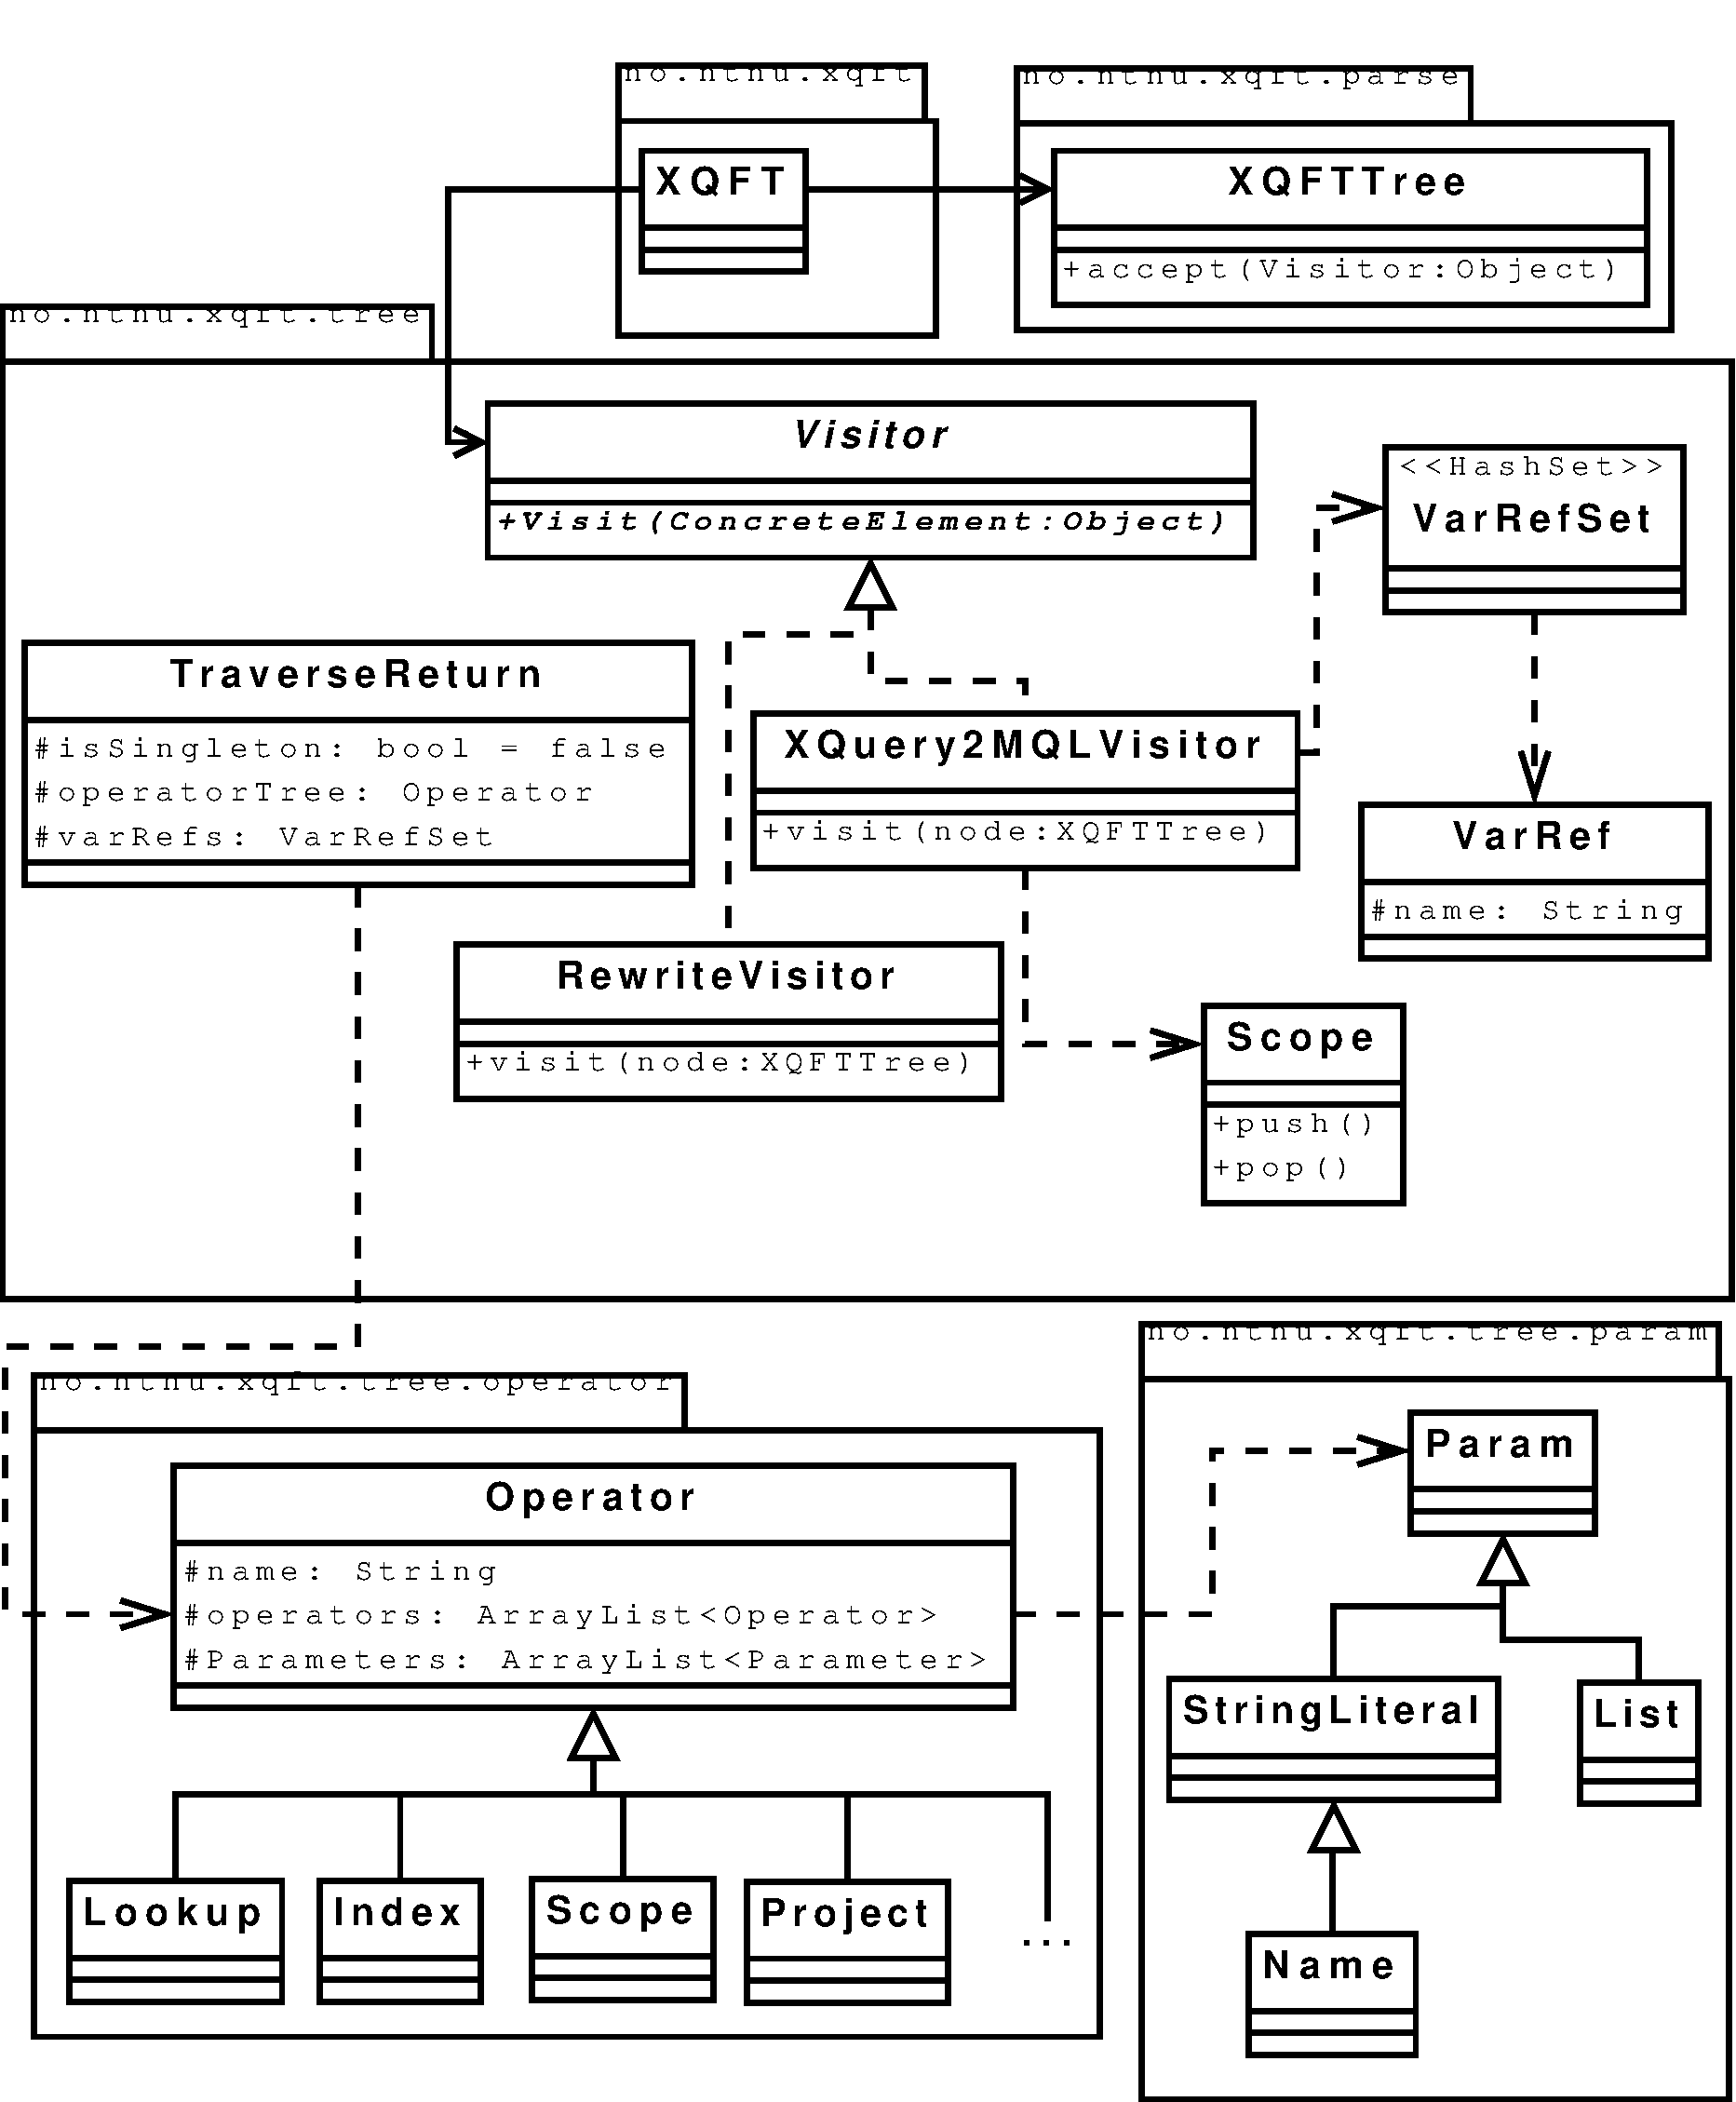
\includegraphics[scale=0.40]{diagrams/complete_uml}
  \caption{Simplified UML for complete implementation}
  \label{fig:impl:sys:uml_complete}
\end{center}
\end{figure}

\subsection{Data flow}
Figure \ref{fig:impl:sys:mql_dataflow} illustrates the flow of data when
translating a XQuery query into a MQL query (see section \ref{sect:method:mql}
on page \pageref{sect:method:mql} for a description of MQL). 

\begin{figure}[!htp]
\begin{center}
  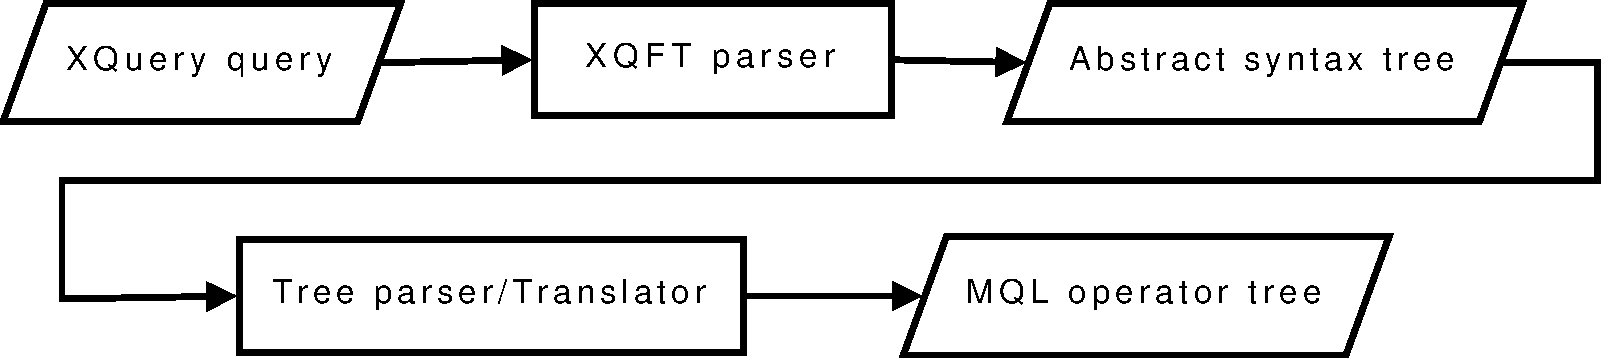
\includegraphics[scale=0.5]{diagrams/mql_dataflow}
  \caption{Data flow for XQuery parsing and translation to MQL}
  \label{fig:impl:sys:mql_dataflow}
\end{center}
\end{figure}

\subsection{Visible external API}
The API available to programmers is defined in a trivial manner in the
\texttt{no.ntnu.xqft.XQFT} class. This class can also be executed as a
standalone application (see next subsection). Figure
\ref{fig:impl:sys:xqft_extapi_uml} describes the \texttt{no.ntnu.xqft.XQFT}
class.

\begin{figure}[!htp]
\begin{center}
  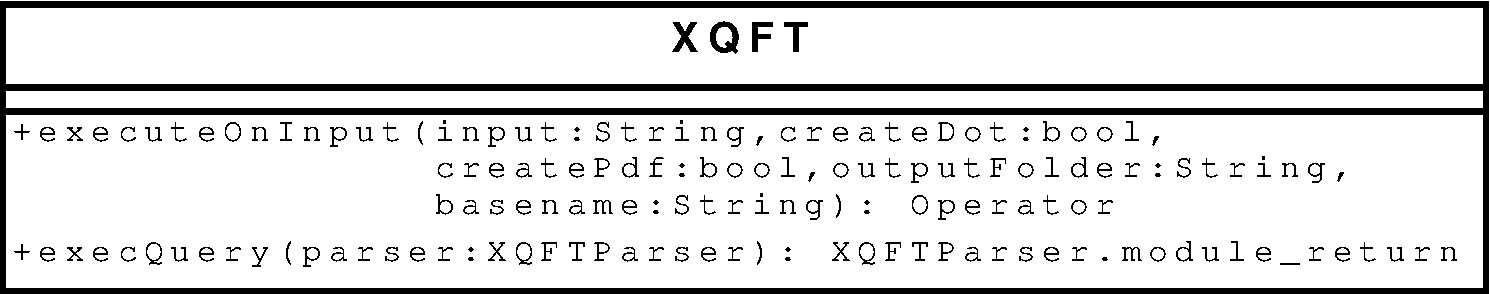
\includegraphics[scale=0.5]{diagrams/xqft_extapi_uml}
  \caption{External API for the XQuery to MQL translator}
  \label{fig:impl:sys:xqft_extapi_uml}
\end{center}
\end{figure}

As can be seen, two methods are primarily available. Out of these two,
\texttt{executeOnInput()} is the most complex, but also the most flexible. A
typical usage scenario for an external user could be as follows:

\begin{Verbatim}
XQFT xqft = new XQFT();
Operator mqlTree = xqft.executeOnInput(
                       "for $i in (1,2,3) return $i", 
                       false, false, null, null
                   );
\end{Verbatim}

The \texttt{mqlTree} would now be a reference to a complete MQL operator tree,
provided that no errors occured during the parse process or the translation
process.

\subsection{Command line interface}
\label{sect:impl:system:cli}
The command line interface is available by executing the
\texttt{no.ntnu.xqft.XQFT} class as a main class, as mentioned in the previous
section. The command line interface uses the Args
Engine\footnote{http://www.adarshr.com/papers/args} for the sake of simplicity
to parse options/switches on the command line. 

The command line usage is as follows:

\begin{verbatim}
java no.ntnu.xqft.XQFT [-p] [-t] [-o <path>] file1 file2 ... fileN
\end{verbatim}

It is also possible to specify queries in the form of strings enclosed in
double quotes, or any mix of strings and filenames. The switches are:
\begin{itemize}
  \item \texttt{-t} : output a DOT tree (requires graphviz)
  \item \texttt{-p} : output a PDF syntax tree (requires graphviz)
  \item \texttt{-o} \texttt{<path>} : stores generated PDF/DOT files in the given folder, 
  otherwise in the current folder (simply \texttt{./})
\end{itemize}

See appendix \ref{appendix:installation} for more information about installation and
dependencies.

\section{Using the XQFT Parser}
The \textit{XQFT Parser}\cite{ourselves} (described in section
\ref{sect:theory:xqftparser}) is a prerequisite for providing the abstract
syntax tree for this XQuery translator. This section will outline how this
parser was used and interfaced with the implementation.

\subsection{Basics and API}
The \textit{XQFT Parser} is a parser generated by the ANTLR parser generator.
Thus, there is a loosely standardised API available for any implementor
utilising a parser generated by ANTLR. In the case of \textit{XQFT Parser}, two
classes are generated: \texttt{XQFTParser} and \texttt{XQFTLexer}. These
classes are used in conjunction on an input string to produce an abstract syntax
tree (see next subsection, and also section
\ref{sect:theory:xqftparser:ast_construction}).

A typical use case to achieve this is shown in figure \ref{}

\begin{figure}[!htp]
\begin{center}
  \begin{Verbatim}
    CharStream cs 
        = new ANTLRStringStream(
            "for $i in (1,2,3) return $i");

    XQFTLexer lexer = new XQFTLexer(cs);

    UnbufferedCommonTokenStream tokens 
        = new UnbufferedCommonTokenStream();
	tokens.setTokenSource(lexer);

    XQFTParser parser = new XQFTParser(tokens);
    parser.setTreeAdaptor(new XQFTTreeAdaptor());
    parser.setLexer(lexer);

    XQFTTree ast = parser.module().getTree();
  \end{Verbatim}
  \caption{Using the XQFTParser and XQFTLexer classes}
  \label{figure:impl:using_xqft}
\end{center}
\end{figure}

\subsection{The XQFTTree class}
\subsection{Interfacing the XQFT Parser}
\section{Constructing the MQL algebra tree}
\label{sect:impl:construct_mql}
The MQL queries are constructed as a tree of operators bottom-up while parsing
the abstract syntax tree (for the corresponding XQuery query). 

\subsection{Operators and parameters}
\begin{figure}[!htp]
\begin{center}
  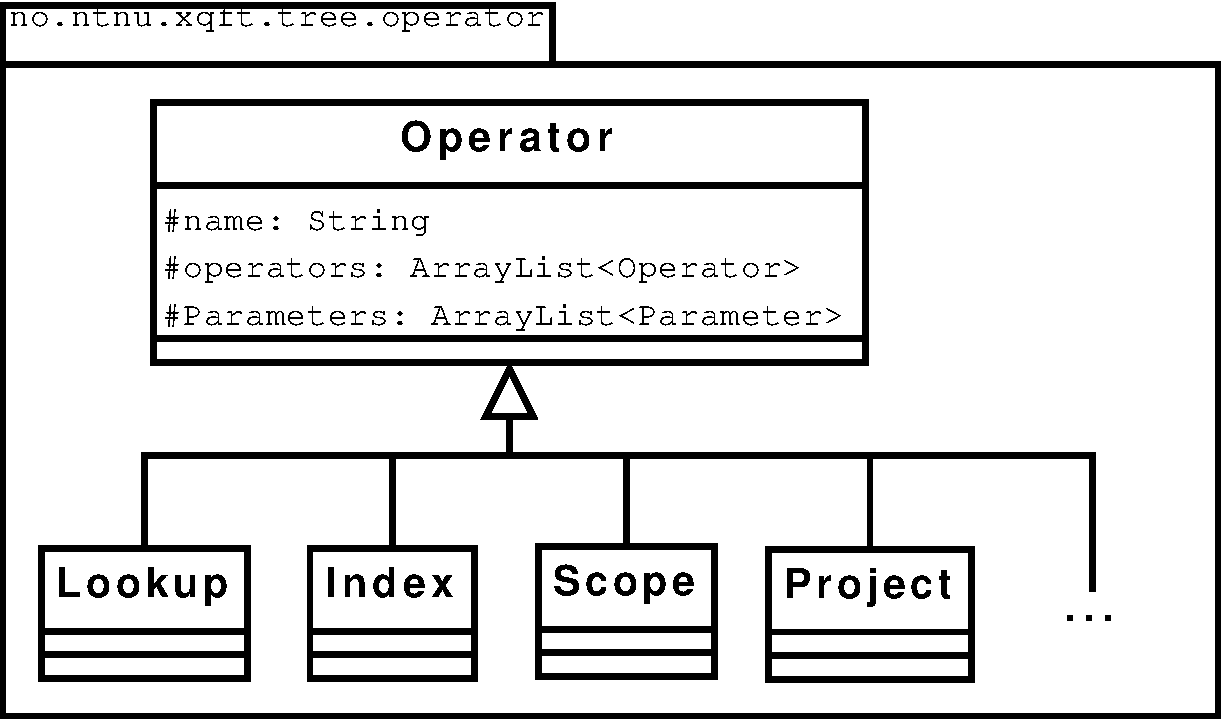
\includegraphics[scale=0.5]{diagrams/mql_operator_uml}
  \caption{Simplified class diagram of MQL operators}
  \label{fig:impl:mql_op_uml}
\end{center}
\end{figure}
The operators modeled in the implementation correspond to the operators
described in section \ref{sect:method:marsOperators}. A simplified class
diagram is shown in figure \ref{fig:impl:mql_op_uml}. Note that the
responsibility with regards to converting an operator to a string
representation is largely left to the various subclasses. However, the default
fallback for the \texttt{Operator} class is to return a string of the form
\begin{Verbatim}
operator_name(param1, param2, ..., paramN; 
              operator1, operator2, ..., operatorM)
\end{Verbatim}
This is sufficient in some cases, such as for the model of the \texttt{cross()}
operator.

\begin{figure}[!htp]
\begin{center}
  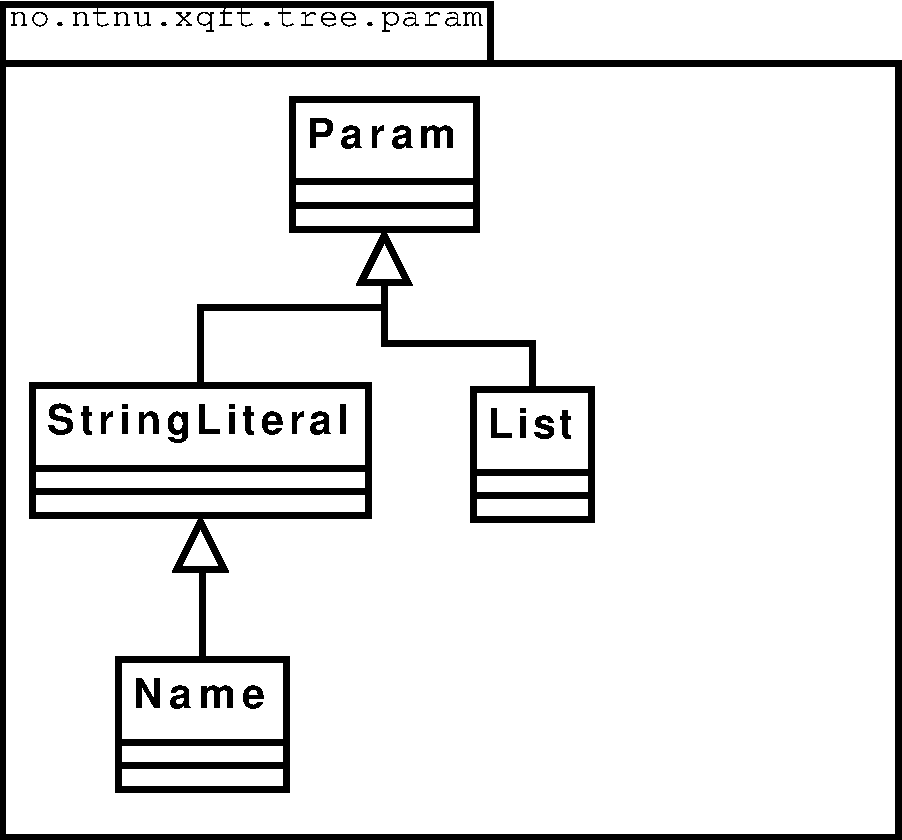
\includegraphics[scale=0.5]{diagrams/mql_param_uml}
  \caption{Class diagram of MQL parameters}
  \label{fig:impl:mql_param_uml}
\end{center}
\end{figure}

MQL parameters (as described in \ref{sect:method:mql:concepts}) are modeled as
seen in figure \ref{fig:impl:mql_param_uml}. Parameters require no complex
structure, and are only created and added to operators as needed.

\subsection{Concepts}
As mentioned, MQL queries are represented as trees, where each node represents
an operator. Each node is an instance of an operator class (as described
above), and contains a list of child operators and a list of parameters. To
convert the operator tree to a MQL query string, simply call the method
\texttt{toPrettyString(0)} on the root node of the operator tree.

\subsection{Usage}
The operator classes are designed to be intuitive and simple to use. Figure
\ref{fig:impl:mql_op_ex1_java} shows one example where a simple operator tree
is built and converted to an MQL query string (the result of which can be seen
in figure \ref{fig:impl:mql_op_ex1_mql}).

%\usepackage{graphics} is needed for \includegraphics
\begin{figure}[htp]
\begin{center}
  \begin{Verbatim}
Lookup lookup = new Lookup("Death in the clouds");
Scope scope = new Scope("/books/book/title", lookup);
Project project = new Project("author", scope);
System.out.println(project.toPrettyString(0));
  \end{Verbatim}
  \caption{Example java code to construct a MQL operator tree}
  \label{fig:impl:mql_op_ex1_java}
\end{center}
\end{figure}

\begin{figure}[htp]
\begin{center}
  \begin{Verbatim}
project([author];
  scope(/books/book/title;
    lookup("Death in the clouds")))
  \end{Verbatim}
  \caption{Resulting MQL query string from example in figure
  \ref{fig:impl:mql_op_ex1_java}}
  \label{fig:impl:mql_op_ex1_mql}
\end{center}
\end{figure}

\section{Context-sensitive visitor}
\label{sect:impl:context_sens_visitor}
In section \ref{sect:theory:parser:tree_parsing} a number of techniques for
tree parsing were presented. In section \ref{sect:method:tree_parsing} the
\textit{context-sensitive visitor pattern} was chosen as the technique for this
implementation. This section will detail the implementation of this design
pattern, and how it is used to performed an assortment of tasks.

\subsection{Basics}
The context-sensitive pattern is designed to be flexible and to generate code
with a higher level of maintainability, for which the rationale was presented
in section \ref{sect:theory:contextVisitorPattern}. 

\begin{figure}[htp]
\begin{center}
  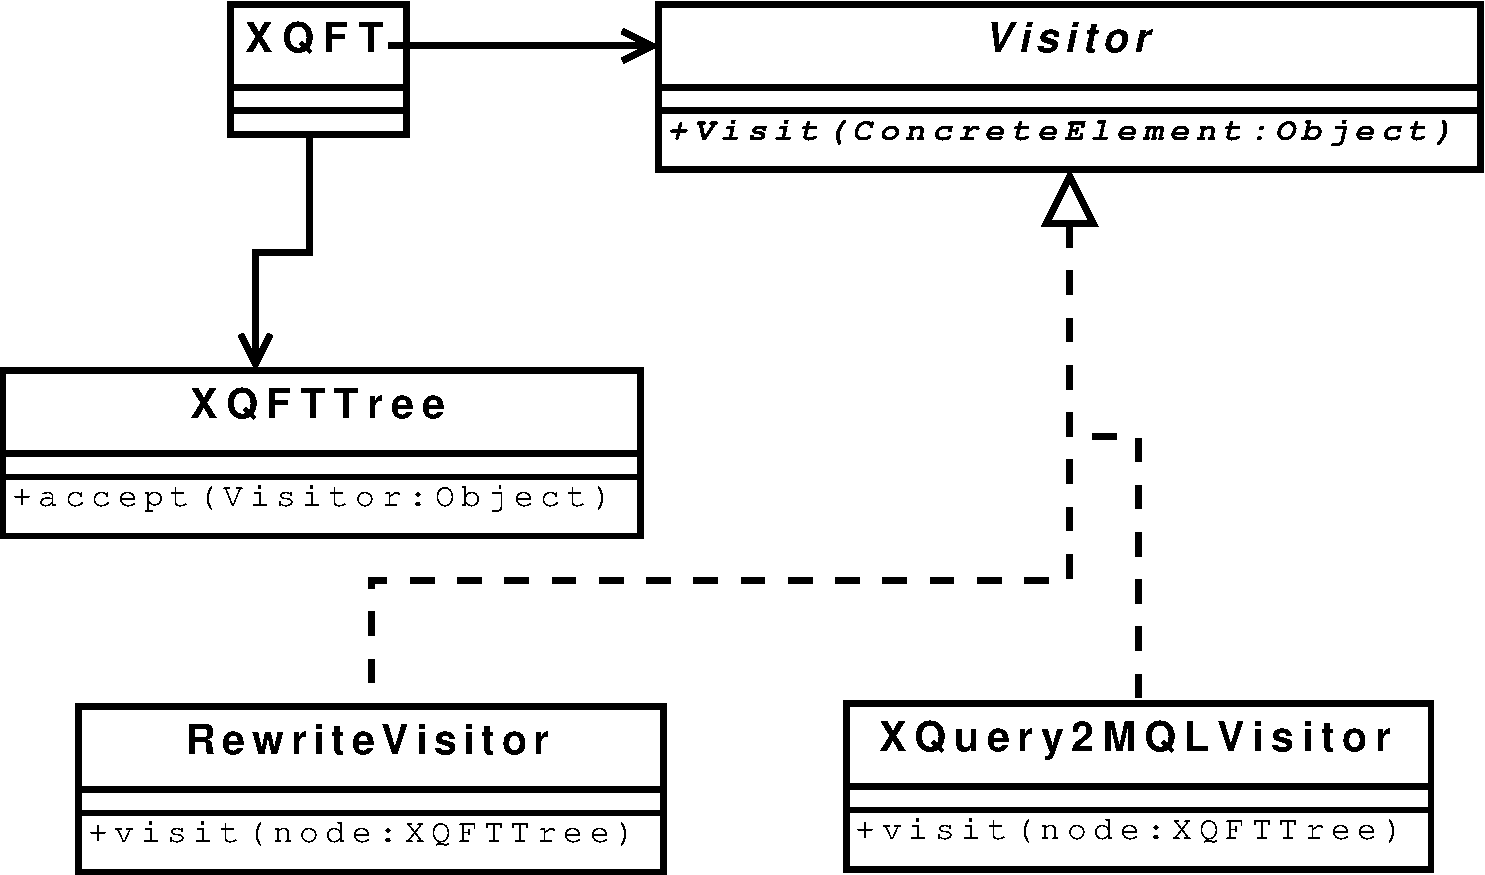
\includegraphics[scale=0.5]{diagrams/context_visitor_pattern_impl}
  \caption{Context sensitive visitor implementation}
  \label{fig:impl:context_sens_visitor_impl}
\end{center}
\end{figure}

The class diagram for the actual implementation of the context-sensitive
visitor pattern can be seen in figure \ref{fig:impl:context_sens_visitor_impl}.
Compare this to the generalized class diagram in figure
\ref{figure:parser:context_visitor_pattern} on page
\pageref{figure:parser:context_visitor_pattern}.

Note that the use of \texttt{XQFTTree} as the element class implies that the
\texttt{XQFTTree} be supplemented with an \texttt{accept()} method to
accommodate this pattern. This method is essentially a static dispatcher which
will call the appropriate method on the visitor based on the token type of the
node currently being visited. Figure \ref{} shows an excerpt of this method and
how it acts on the visitor class.

%\usepackage{graphics} is needed for \includegraphics
\begin{figure}[htp]
\begin{center}
  \begin{Verbatim}	
public TraverseReturn accept(Visitor visitor) {
     case XQFTParser.AST_MODULE:
            return visitor.visitAST_MODULE(this);
        case XQFTParser.AST_FLWOR:
            return visitor.visitAST_FLWOR(this);
        case XQFTParser.AST_FORCLAUSE:
            return visitor.visitAST_FORCLAUSE(this);
        case XQFTParser.AST_LETCLAUSE:
            return visitor.visitAST_LETCLAUSE(this);
        case XQFTParser.AST_ORDERBYCLAUSE:
            return visitor.visitAST_ORDERBYCLAUSE(this);
        case XQFTParser.AST_WHERECLAUSE:
            return visitor.visitAST_WHERECLAUSE(this);
                          .
                          .
                          .
  \end{Verbatim}
  \caption{Excerpt from the accept() method in the XQFT class}
  \label{figureLabel}
\end{center}
\end{figure}

\subsection{The Rewrite visitor}
The \textit{Rewrite visitor} is used to perform rewrite operations on the
abstract syntax tree before performing the actual translation. In particular,
these rewrite operations consists of normalizing the required subtrees of the
syntax tree to a subset of XQuery Core (as described in sections
\ref{sect:theory:xquery:XQcore} and \ref{sect:method:ast_rewrite}).

\subsection{The XQuery2MQL visitor}
The \textit{XQuery2MQL visitor} performs the bulk of the work related to
performing the translation of XQuery to MQL. This visitor is capable of
re-instantiating itself (or other visitors) when entering new contexts, such as
path predicates. 
\section{Scoping and Symbol Tables}
Crucial to the implementation of the Tainting Dependencies (TD) methodology
described in chapter \ref{chapter:translation} is the ability to
maintain a contextual environment with scoping and symbol tables. This section
details the implementation of this, and how it is used to meet the
requirements of TD.

\subsection{Concepts}
The scoping system in the implementation is based on building a scope tree. The
previous scope, if any, is set as parent of the new scope, and the previous
scope maintains a list of child scopes -- this is referred to as
\textit{pushing a scope}. When exiting a scoped subexpression in the AST, the
previous scope is again set as the current scope. This is referred to as
\textit{popping a scope}. A reference to the root scope node is always
maintained. Considering the example XQuery query in figure
\ref{fig:impl:scope_tree_ex_code}, the scope tree in figure
\ref{fig:impl:scope_tree_ex} is generated. The scope itself contains \emph{one}
symbol table for the current scope.

\begin{figure}[!htp]
\begin{center}
\begin{minipage}[h]{9cm}
\begin{verbatim}
for $i in (1,2,3) return 
  for $a in (4,5,for $b in (6,7,8) return $b) 
    return ($i,$a)
\end{verbatim}
  \caption{Scope tree example code}
  \label{fig:impl:scope_tree_ex_code}
  \end{minipage}
\end{center}
\end{figure}

\begin{figure}[!htp]
\begin{center}
  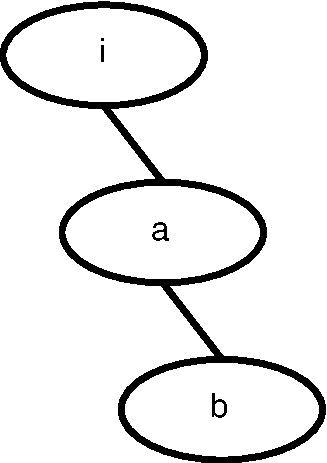
\includegraphics[width=0.2\textwidth]{diagrams/scope_tree_ex}
  \caption{Scope tree for source code in figure
  \ref{fig:impl:scope_tree_ex_code}} 
  \label{fig:impl:scope_tree_ex}
\end{center}
\end{figure}

Entries in the symbol table are represented through an instance of the
\texttt{SymTabEntry} class which maintains metadata about symbols (such as
symbol name, a flag indicating whether it's an iterator variable, and an
evaluated expression). The symbol table is realised as a subclass of the
\texttt{HashMap} class in the \texttt{java.util} package, and is constrained to
storing instances of \texttt{SymTabEntry}, with the symbol name as key.

\subsection{Semantics}
The scoping semantics are encapsulated in a singleton manner in the class
\texttt{Scope}, with static methods available for pushing and popping scopes,
and storing and retrieving symbols. The external (static) API as available to a
user of the scope system is shown in figure \ref{fig:impl:scope_uml}.

\begin{figure}[!htp]
\begin{center}
  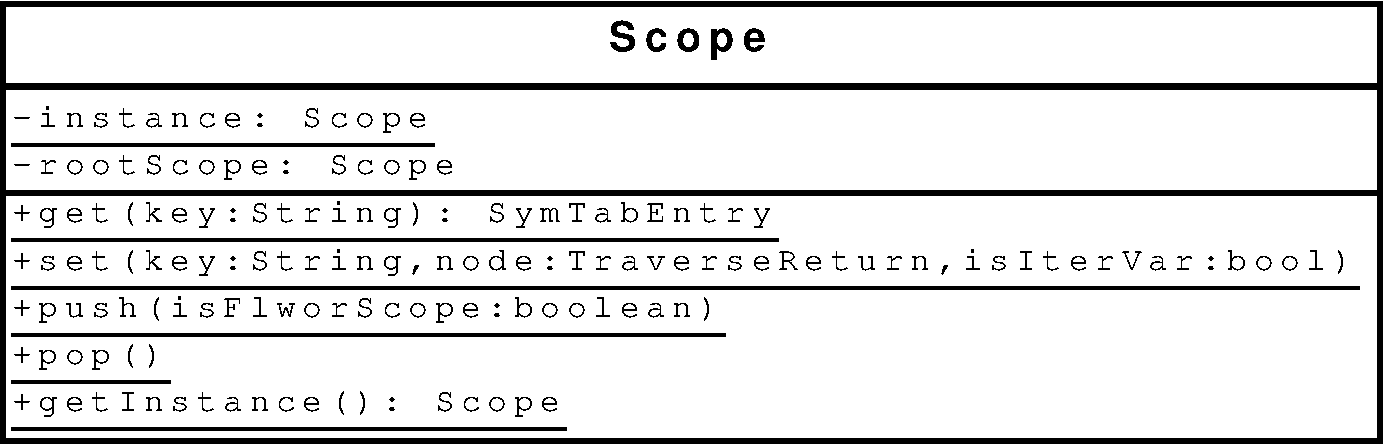
\includegraphics[width=0.7\textwidth]{diagrams/scope_uml}
  \caption{Scope API}
  \label{fig:impl:scope_uml}
\end{center}
\end{figure}

A new scope is \textit{pushed} whenever a \texttt{for}-clause is encountered while
parsing the abstract syntax tree, and the current scope is \textit{popped} after
evaluating a \texttt{return}-clause -- both of which occur within a FLWOR expression.

The scoping system also tracks iteration variables. That is, for any scope,
there is \textit{one and only one} iteration variable, except in the top scope
where there is no iteration variable. The concept of an iteration variable is
explained in definition \ref{def:iterVarDep}. Tracking of these
variables are reviewed in section \ref{sect:impl:tainting_deps}.
\section{Passing Metadata Between Nodes}
To implement the Tainting Dependencies method it is necessary to pass
metadata upwards when parsing the syntax tree, such as
iterator dependencies and flags to indicate singleton nodes (for simplifications). Additionally, the
operator tree which is being built bottom-up (as described earlier in section
\ref{sect:impl:construct_mql}) is also required to be passed upwards. 

This is achieved through the \texttt{TaverseReturn}, which models a return type
when visiting nodes in the syntax tree. That is, the visitor methods are
responsible of 1) visiting any child nodes, and 2) returning an instance of the
\texttt{TraverseReturn} class based on what was returned from the child nodes,
if anything.

\subsection{The TraverseReturn Class}
The class diagram for the \texttt{TraverseReturn} class is shown in figure
\ref{fig:impl:meta:traverse_uml}. Note the flag to indicate if the current
context is a singleton, the reference to an MQL operator tree (which is being
built bottom-up), and a reference to a set of iterator dependencies (in the implementation called
\texttt{varRefs}).

\begin{figure}[!htp]
\begin{center}
  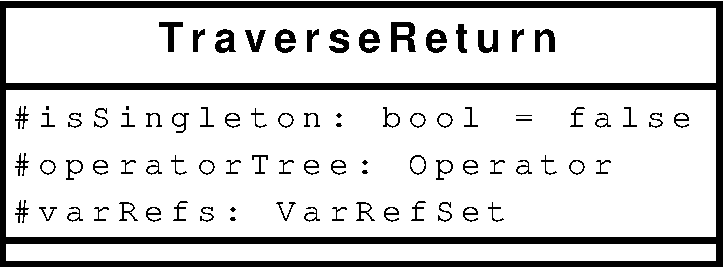
\includegraphics[scale=0.5]{diagrams/traversereturn_uml}
  \caption{TraverseReturn class diagram}
  \label{fig:impl:meta:traverse_uml}
\end{center}
\end{figure}

The \texttt{TraverseReturn} class is, as mentioned, used in the visitor when
visiting nodes in the abstract syntax tree (see section
\ref{sect:impl:context_sens_visitor}). A typical use case is shown in figure
\ref{fig:impl:meta:traverse_usage_ex}, which is an excerpt from the
implementation.

\subsection{Iterator Dependencies}
Iterator dependencies, described in section \ref{sect:trans:TD:basics}, are
passed upwards together with the MQL operator tree being built during the syntax
tree parsing process. These sets of dependencies are handled by th \texttt{VarRef} and \texttt{VarRefSet} classes.
A class diagram for these classes is shown in figure \ref{fig:impl:meta:varrefset_uml}.

\begin{figure}[!htp]
\begin{center}
  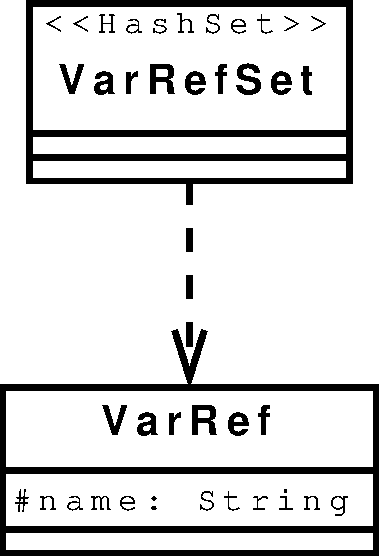
\includegraphics[scale=0.5]{diagrams/varrefset_uml}
  \caption{\texttt{VarRefSet} and \texttt{VarRef} class diagram}
  \label{fig:impl:meta:varrefset_uml}
\end{center}
\end{figure}

As described in section \ref{sect:trans:TD:dependency}, an iterator variable reference is always dependent on
its corresponding iterator. Thus, when a iterator variable is encountered during the parse process, and the
variable is being ``read'' and not assigned or declared, the corresponding iterator is added to the current set of
iterator dependencies. The example in figure \ref{fig:impl:meta:var_ref_ex} shows the variable \texttt{\$a}
being read, in which case the iterator is added to the \texttt{TraverseReturn}
to-be-returned's set of dependencies.

\begin{figure}[!htp]
\begin{center}
\begin{minipage}[h]{5cm}
\begin{verbatim}
for $i in (1,2,3) return 
    ($a,4,5)
\end{verbatim}
\end{minipage}
  \caption{Example of the variable \texttt{\$a} being read. Note that the iterator
  variable \texttt{\$i} is never read}
  \label{fig:impl:meta:var_ref_ex}
\end{center}
\end{figure}

The source code excerpt in figure \ref{fig:impl:meta:var_ref_impl2} shows how
iterator dependencies are treated in the visitor implementation.

\begin{figure}[!htp]
\begin{center}
\begin{Verbatim}
// Fetch entry from symtab
SymTabEntry entry = Scope.get(tree.getChild(0).getText());
            
// Obtain and append new var ref
TraverseReturn tr = entry.getTraverseReturn();
tr.getVarRefs().add(new VarRef(tree.getChild(0).getText()));

return tr;
\end{Verbatim}
  \caption{Appending a new variable reference}
  \label{fig:impl:meta:var_ref_impl2}
\end{center}
\end{figure}

\subsection{Singleton nodes}
Singleton nodes are nodes corresponding to expressions that return a sequence of exactly one item. In
the cases where this is known to be true, the result from a translation can be
tagged with this information and used later to simplify the translation of
sequence construction (as described in section \ref{sect:impl:td:seq}).

This is the case of integer literal nodes as well as iterator variable lookups in the
symbol table. The case of integer literal nodes is shown in figure
\ref{fig:impl:meta:traverse_usage_ex} in the next section. The case of variable
lookups is somewhat less intuitive, since the singleton flag is actually
stored when a variable is first set. That is, the right-hand side of the
assignment is translated once and annotated with the singleton flag, which is
then set for all subsequent lookups in the symbol table. The excerpt in figure 
\ref{fig:impl:meta:var_assign_ex} shows how this is done in the implementation.

\begin{figure}[!htp]
\begin{center}
\begin{Verbatim}
// Visit children on the right side of the assignment
TraverseReturn tr = acceptThis(tree.getChild(1));

// Required for tainting deps method
Project project = new Project("[" + varName + "numb, value]", 
                      tr.getOperatorTree());

// Assign metadata
tr.setOperatorTree(project);
tr.setSingleton(true);

// Enter into symbol table
SymTabEntry tmp = Scope.set(tree.getChild(0).getText(), 
                      tr, isIterationVar);
\end{Verbatim}
  \caption[Iterator variable annontion with singleton flag]{Iterator variable
  assignment example, annotated with the singleton flag before being entered into the symtab}
  \label{fig:impl:meta:var_assign_ex}
\end{center}
\end{figure}

\subsection{Example of usage}
In the example in figure \ref{fig:impl:meta:traverse_usage_ex}, an
integer literal node is visited (a node that simply holds an integer). A
\texttt{make()} MQL operator as well as a new \texttt{TraverseReturn}
instance is created. The \texttt{make()} operator is then appended to the 
\texttt{TraverseReturn} instance, and the \textit{isSingleton} flag is set to 
\textit{true} since the result of this translation is a single item.

\begin{figure}[!htp]
\begin{center}
\begin{Verbatim}
public TraverseReturn visitIntegerLiteral(XQFTTree tree) {

    Make make = new Make("name:=[index, value], [1, " + tree.getText());
    TraverseReturn tr = new TraverseReturn();        
    tr.setSingleton(true);
    tr.setOperatorTree(make);
    return tr;
}
\end{Verbatim}
  \caption{TraverseReturn usage example}
  \label{fig:impl:meta:traverse_usage_ex}
\end{center}
\end{figure}
\section{Tainting dependencies}
``Tainting dependencies'' is a method of translating XQuery queries to
relational algebra. The semantics of this method is described in detail
throughout section \ref{sect:trans:taintingDependencies}. This section
describes an implementation of a subset of this method which is capable of
translating simple FLWOR expressions, sequences, and variables. 

\label{sect:impl:tainting_deps}
Dette blir den lengste seksjonen i dette kapittelet, h\aa per jeg.
\subsection{FLWOR expressions}



\subsection{Sequences}
\label{sect:impl:td:seq}
\begin{itemize}
  \item behandler parantes istf. komma for sekvenser (ref spec) 
\end{itemize}

\section{Summary}
\label{sect:impl:summary}
This chapter has described the implementation of a proof of concept for the
``Tainting Dependencies'' method. In the next chapter, some results are
presented, such as theoretical algebra output. Additionally, algebra generated
by the prototype described here will be compared to that generated by
Pathfinder.

%\newpage
%\mbox{}

%RESULTS
\chapter{Results}
\label{chapter:results}
This chapter will showcase a series of relational algebra trees. First, in
section \ref{sect:result:theoretical_algebra}, example trees computed by hand
using the rules for ``Tainting Dependencies'' are presented, showcasing
some major capabilities of this method. Further, in section
\ref{sect:result:implementation_algebra}, some trivial and complex queries are
generated by the prototype implementation and displayed. Furthermore, in
section \ref{sect:results:comparison}, comparisons are made to algebra
generated by Pathfinder/MonetDB using classic loop lifting.

\section{Theoretical Algebra}
\label{sect:result:theoretical_algebra}
In this section, a collection of XQuery query examples and their translation to
relational algebra is presented. The translation is done manually using the
``Tainting Dependencies'' method described in chapter \ref{sect:translation}. For the sake of
brevity, only the rules used throughout the translation will be noted. Intermediate results will
not be included.

Generell struktur:
- Sp\oe rring
- Semantikk (resultat)
- Translasjon
- Mellomregninger? (naaii..)

\subsection{Extensive FLWOR}
This example will illustrate the translation of a more complex FLWOR expression.

\subsubsection{Query premise}
\begin{figure}[!htp]
\begin{center}
\begin{Verbatim}
for $a in (1,2,3) let $b := 2
  where $a gt $b
  order by $a
  return ($a, $b)
\end{Verbatim}
  \caption{Extensive FLWOR expression, showcasing for-, let-, where-, orderby-,
  and return-clauses}
  \label{fig:results:query_ext_flwor}
\end{center}
\end{figure}

\subsubsection{Translation process}
The translation process in its entirety is shown step by step in appendix
\ref{appendix:transl:ext_flwor}, page \pageref{appendix:transl:ext_flwor}.

\subsubsection{Result}
The result of the translation is shown in figure
\ref{fig:results:query_ext_flwor_result}.

\begin{figure}[!htp]
\begin{center}
  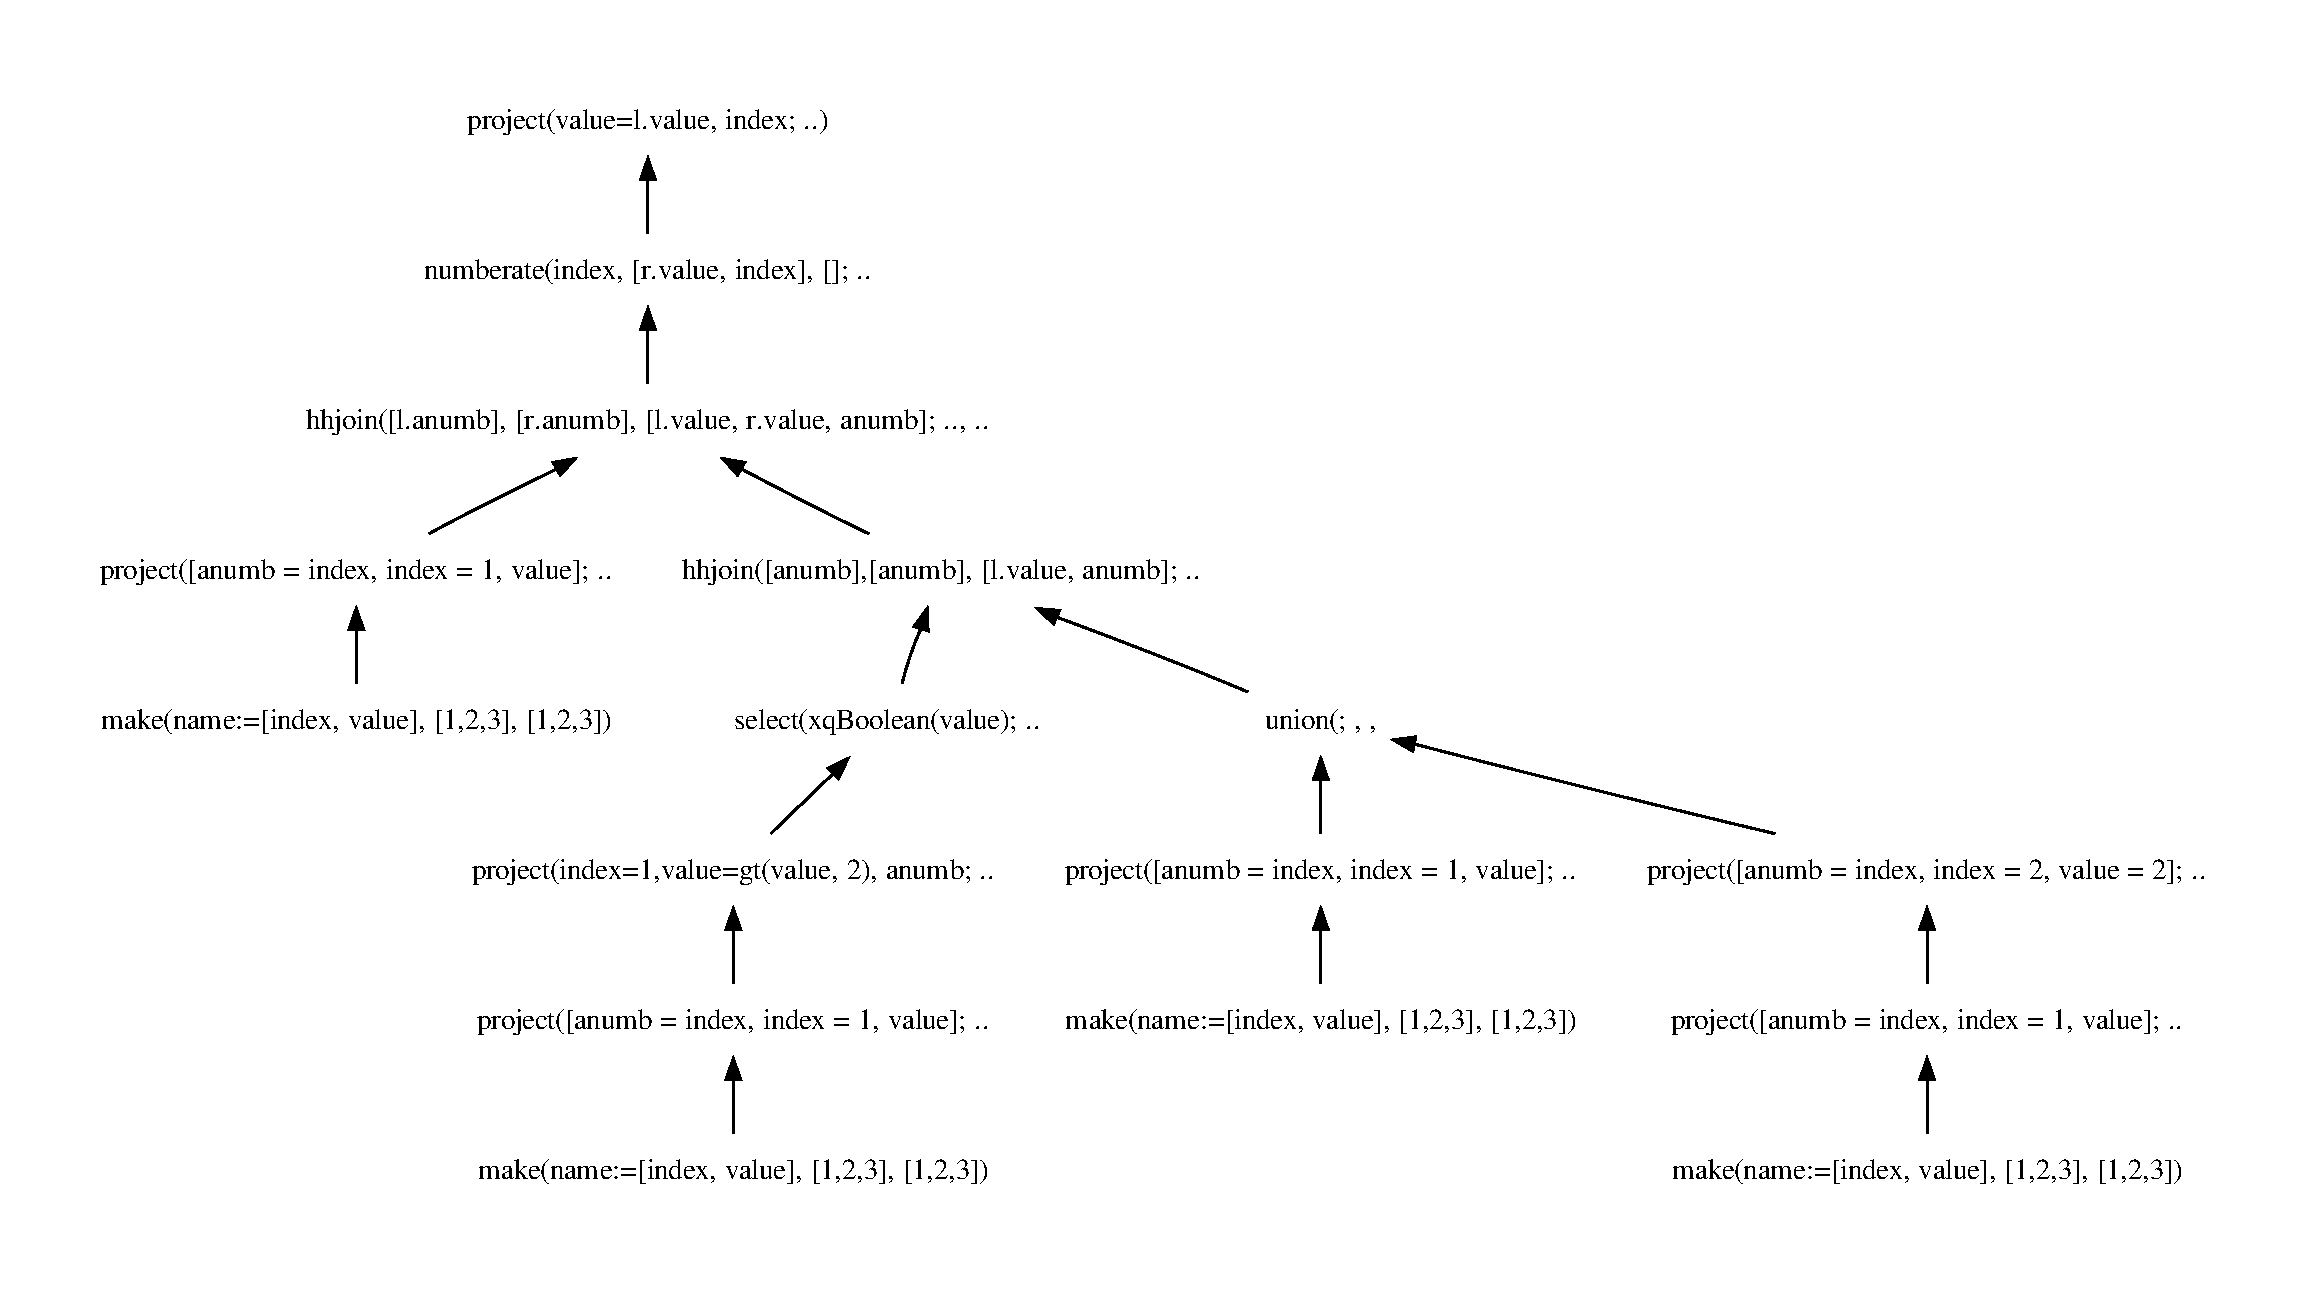
\includegraphics[width=1.0\textwidth]{img/graphs/ext_flwor}
  \caption{Complete translation of expression in figure
  \ref{fig:results:query_ext_flwor}}
  \label{fig:results:query_ext_flwor_result}
\end{center}
\end{figure}

The operator tree in figure \ref{fig:results:query_ext_flwor_result} can be
converted to the DAG seen in figure \ref{fig:results:query_ext_flwor_dag}.

\newpage

\begin{figure}[!htp]
\begin{center}
  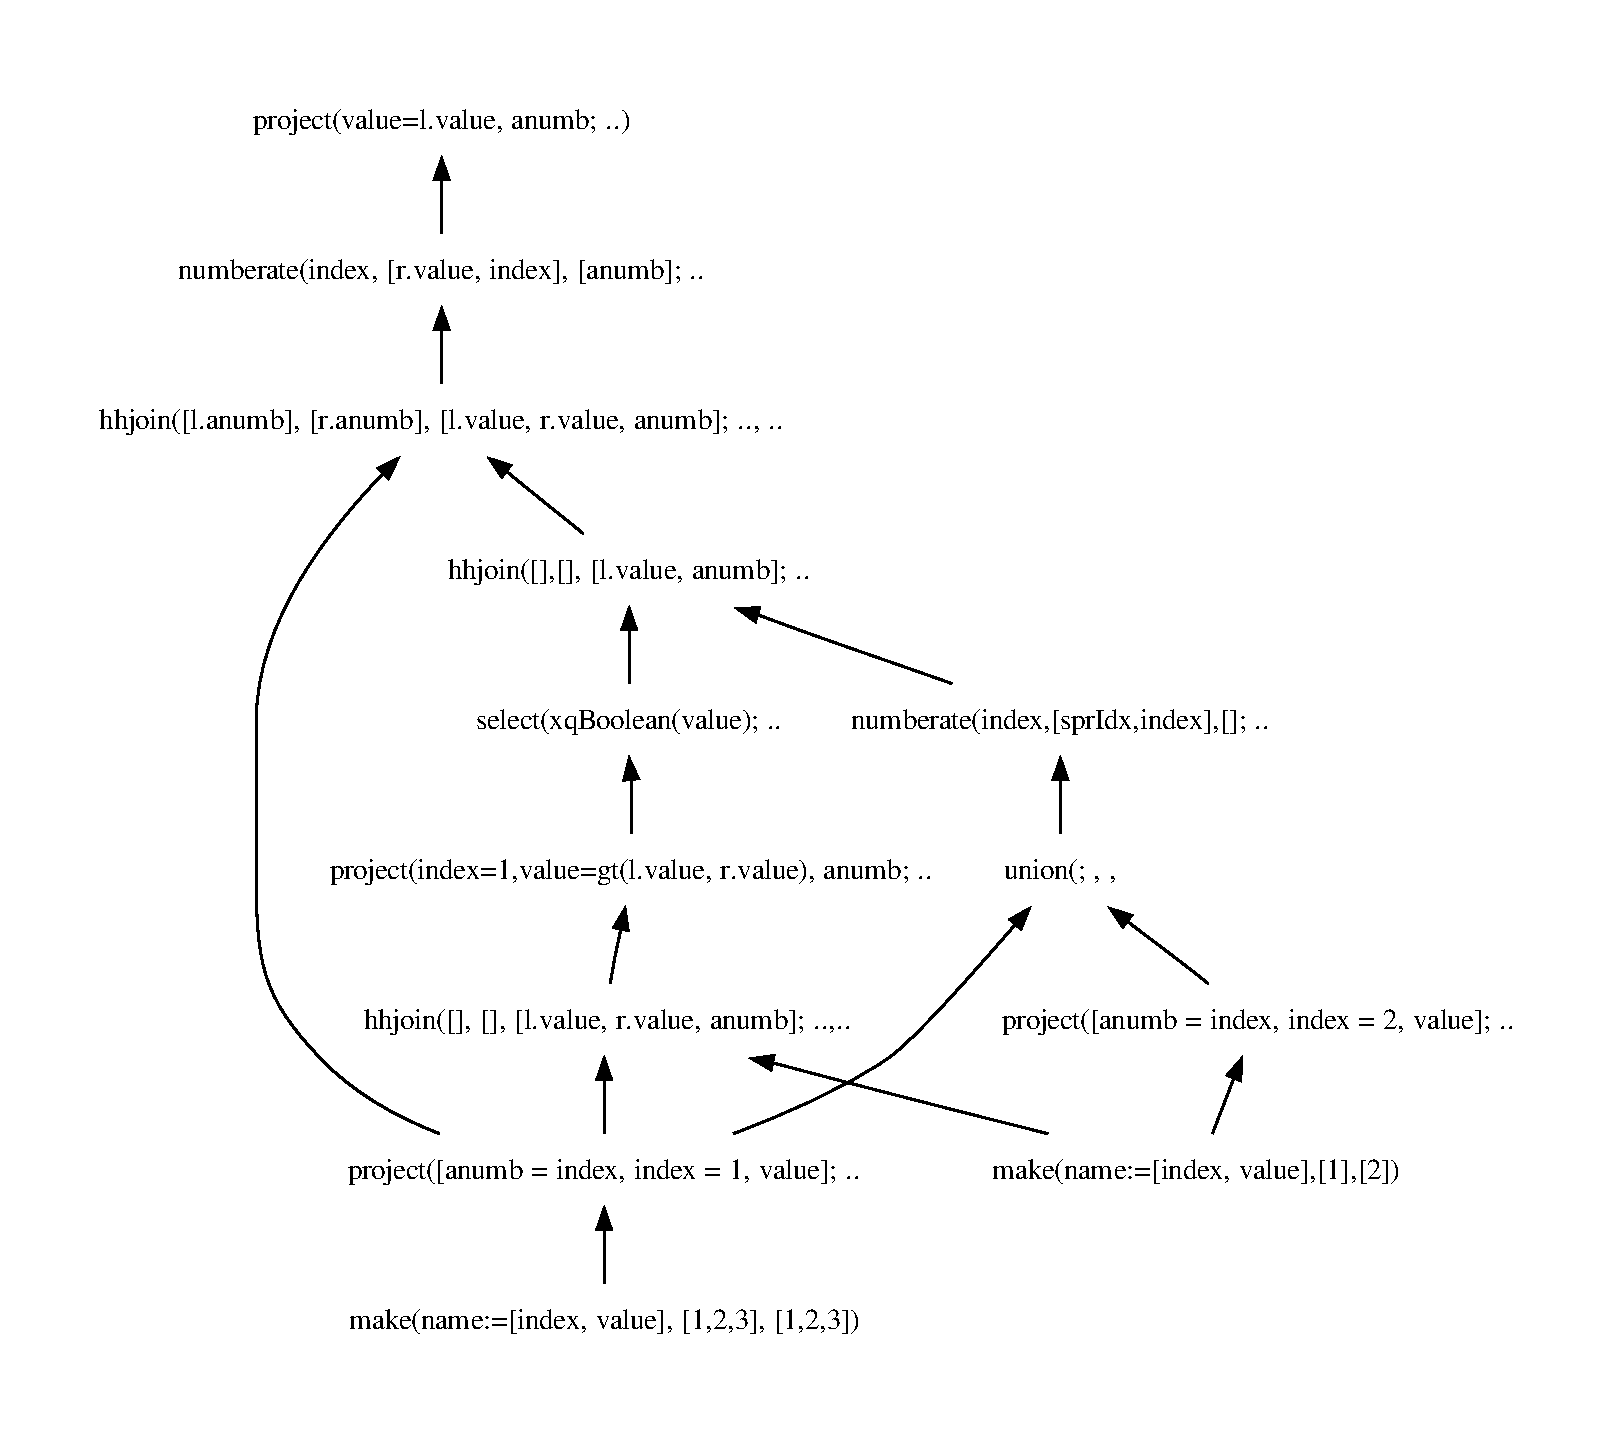
\includegraphics[width=1.0\textwidth]{img/graphs/ext_flwor_dag}
  \caption{DAG representation of operator tree in figure
  \ref{fig:results:query_ext_flwor_result}}
  \label{fig:results:query_ext_flwor_dag}
\end{center}
\end{figure}

\subsection{Path expression with predicate}
This example will illustrate the translation of a path expression with a predicate.

\subsubsection{Query premise}
\begin{figure}[!htp]
\begin{center}
\begin{Verbatim}
/a/b[@id eq 2] 
\end{Verbatim}
  \caption{Path expression with a predicate query premise}
  \label{fig:results:query_pathPred}
\end{center}
\end{figure}

\subsubsection{Translation process}
The translation process in its entirety is shown step by step in appendix
\ref{appendix:transl:pathPred}, page \pageref{appendix:transl:pathPred}.

\subsubsection{Result}
The result of the translation is shown in figure
\ref{fig:results:query_pathpred_result}.

\begin{figure}[!htp]
\begin{center}
  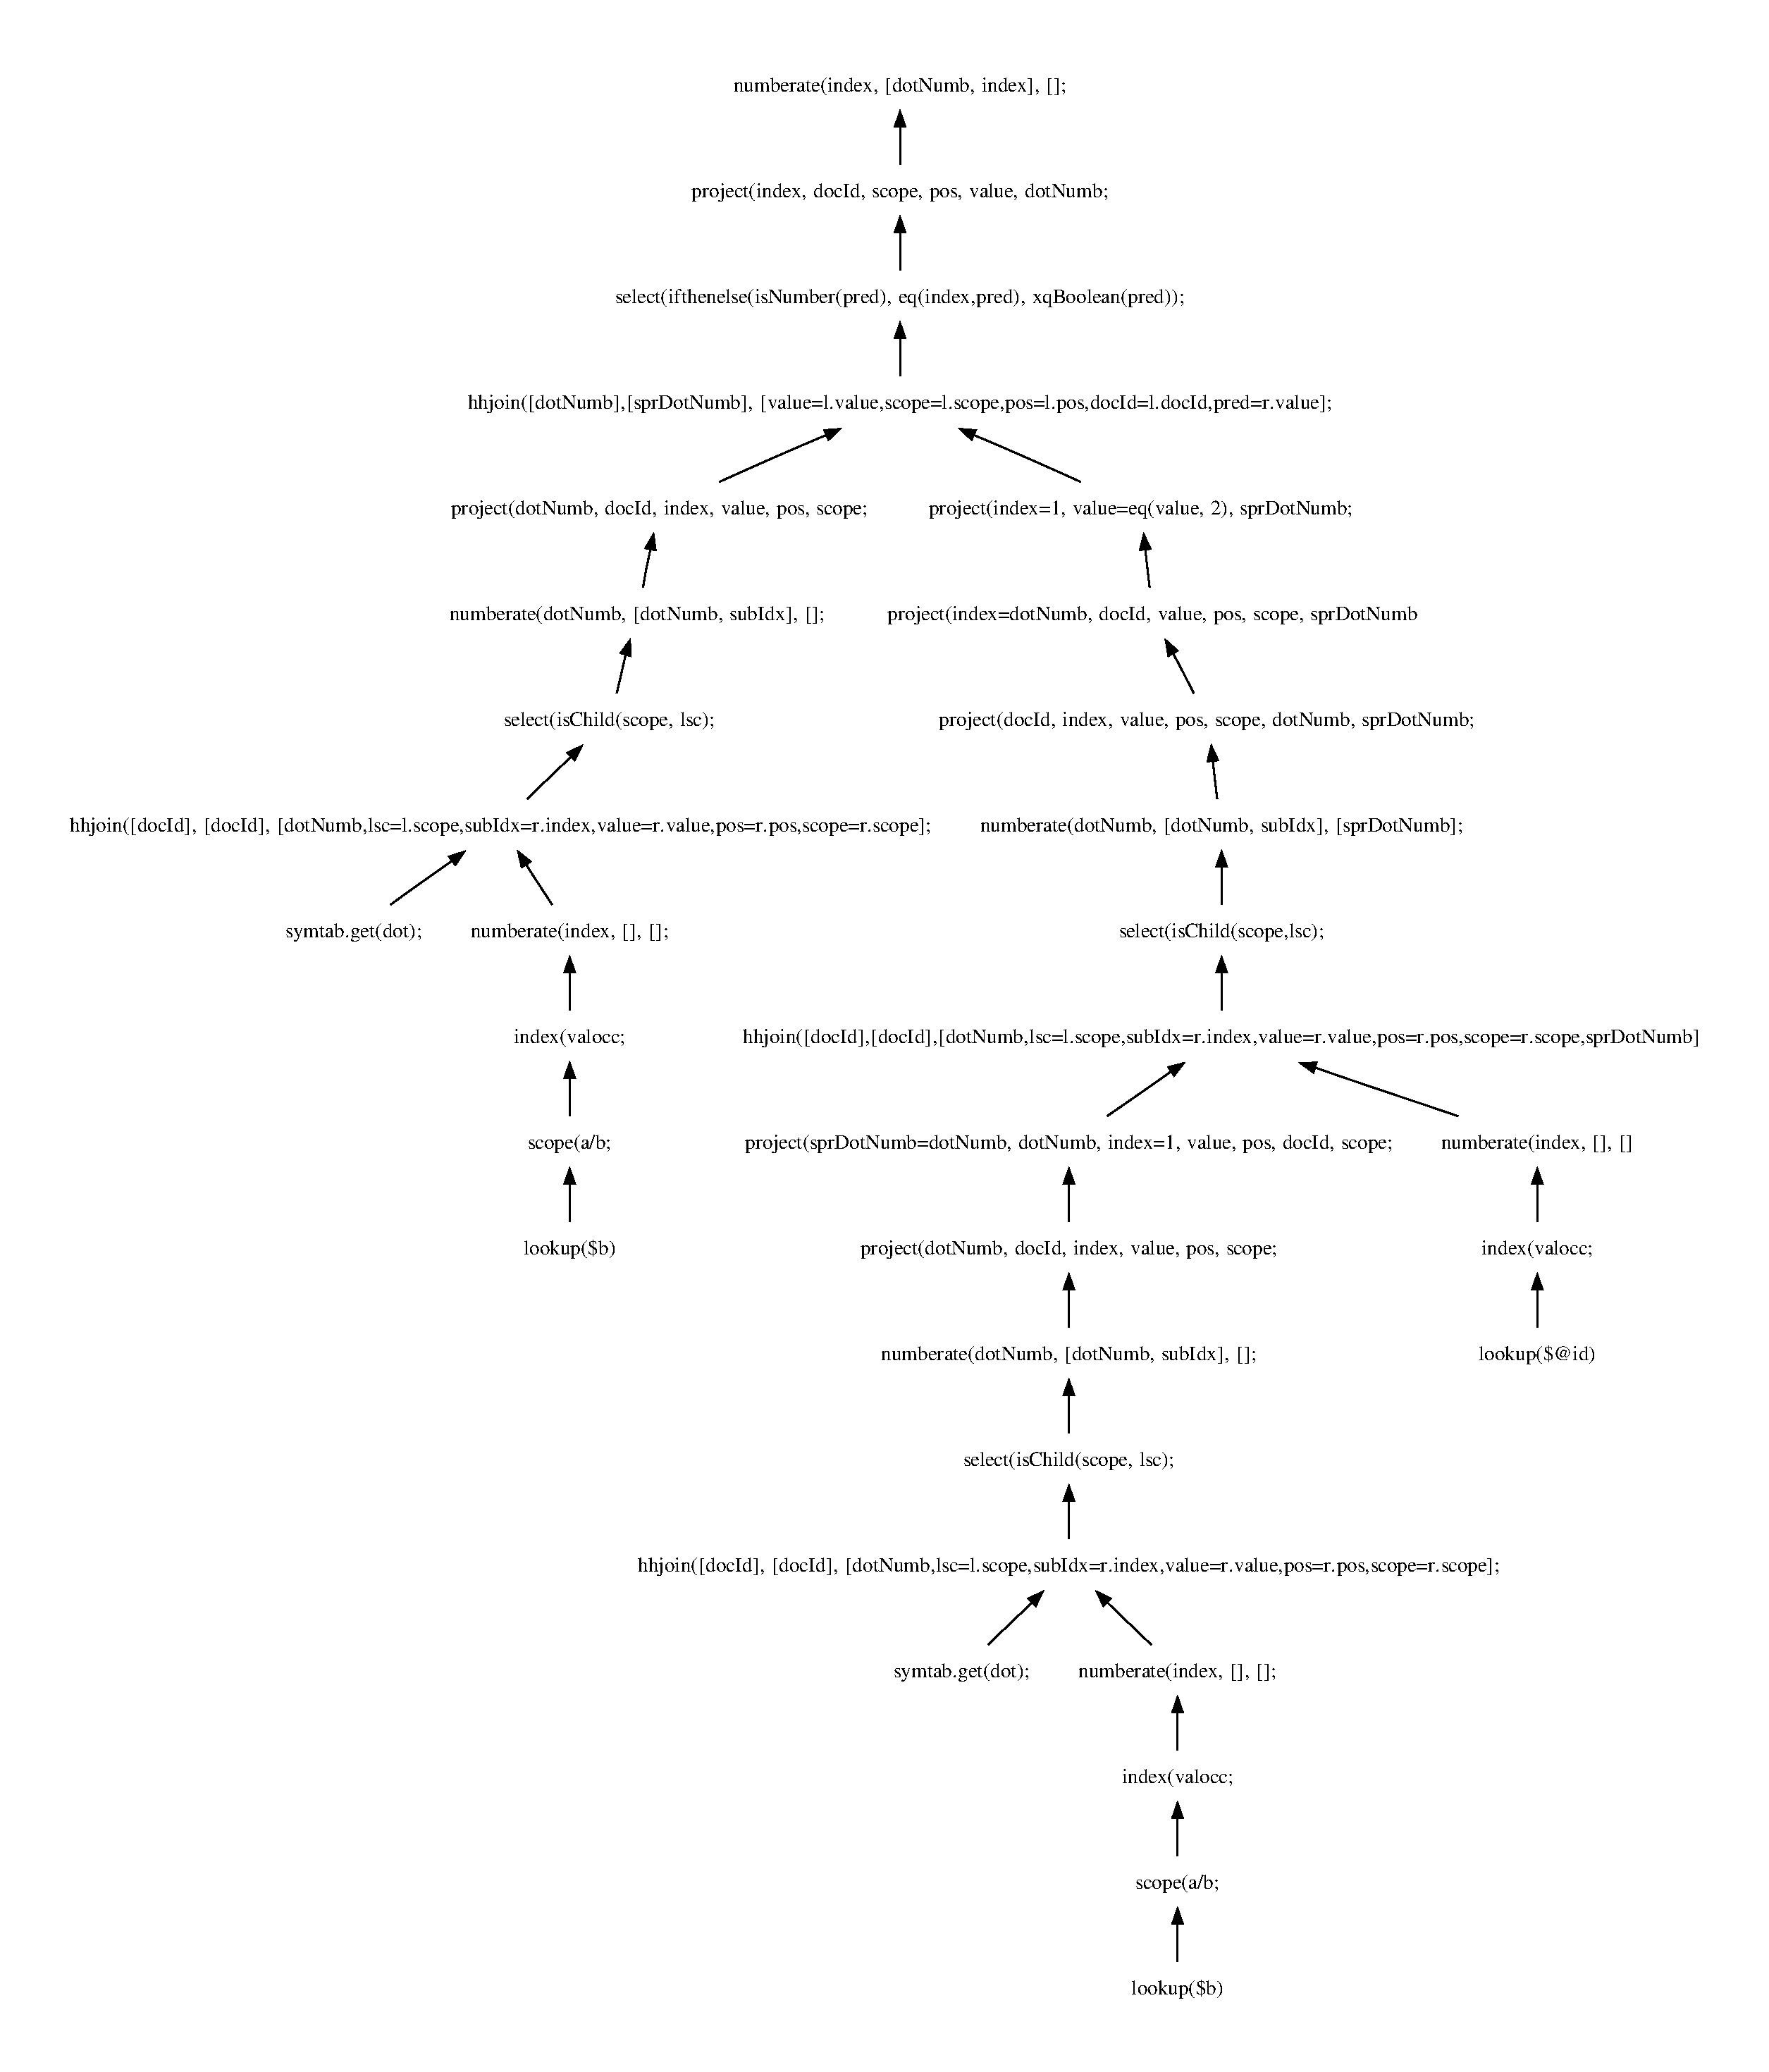
\includegraphics[width=1.0\textwidth]{img/graphs/TD_patExprPred}
  \caption{Complete translation of expression in figure
  \ref{fig:results:query_pathPred}}
  \label{fig:results:query_pathpred_result}
\end{center}
\end{figure}

The operator tree in figure \ref{fig:results:query_pathpred_result} can be
converted to the DAG seen in figure \ref{fig:results:query_pathpred_result_dag}.

\newpage

\begin{figure}[!htp]
\begin{center}
  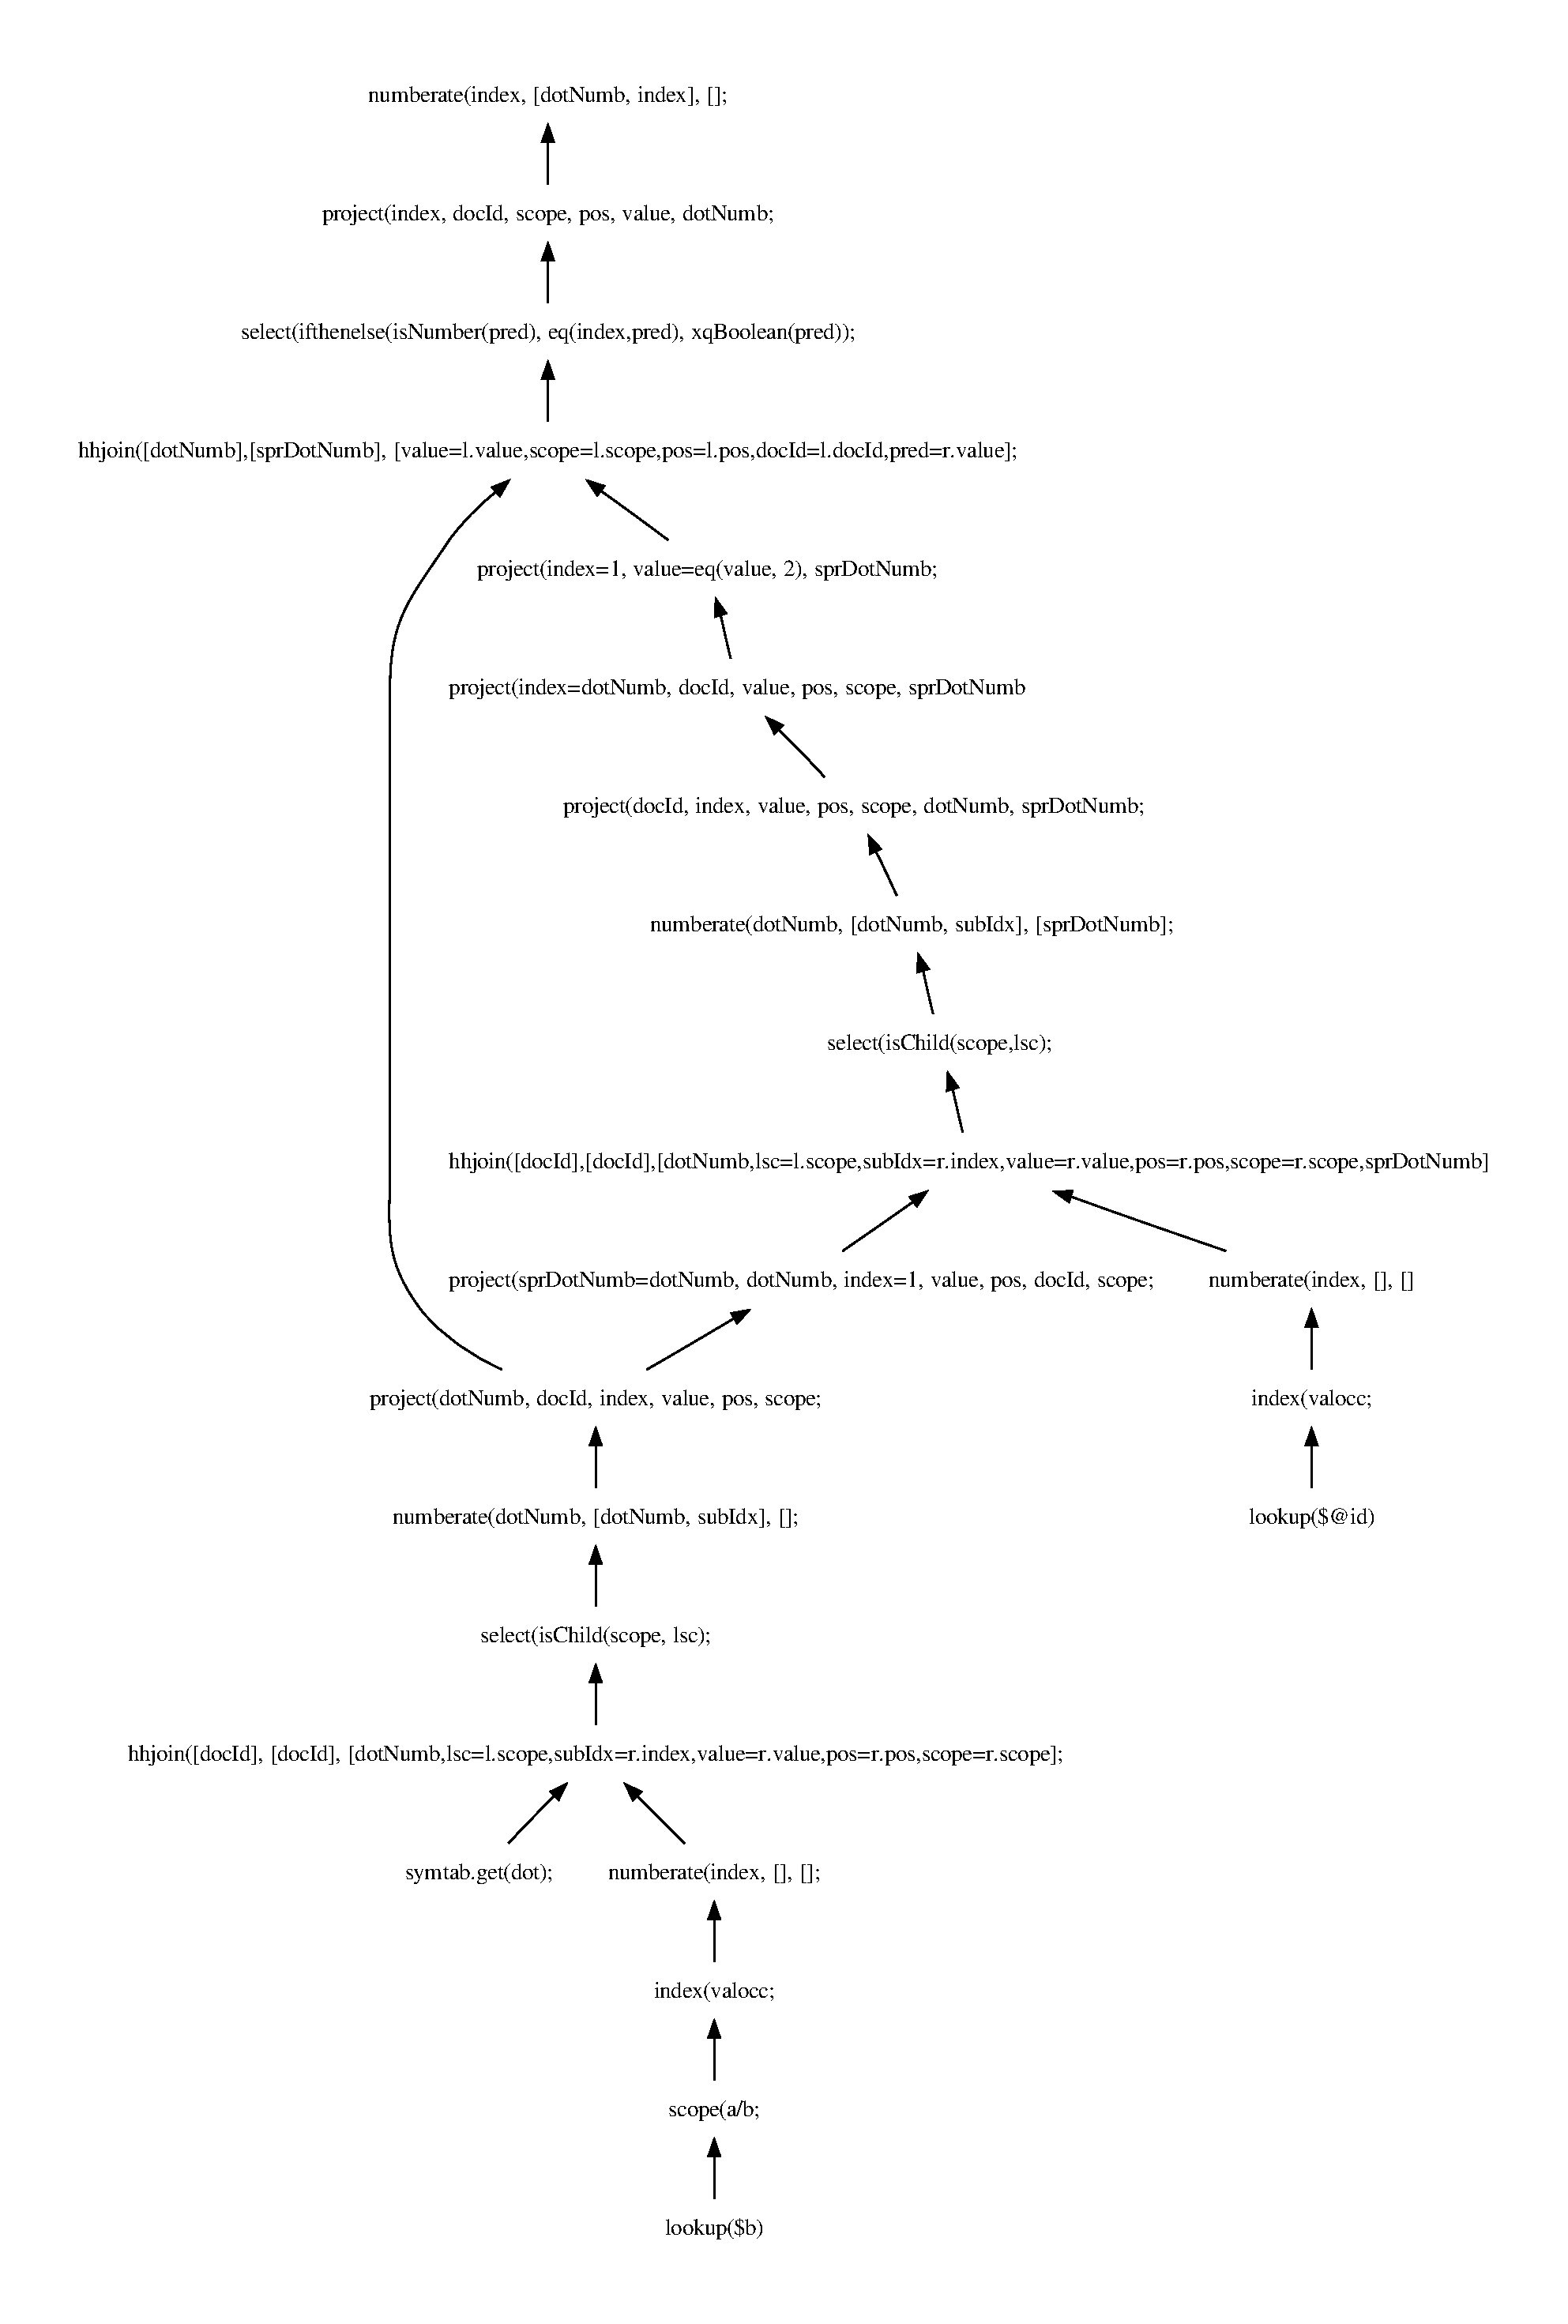
\includegraphics[width=1.0\textwidth]{img/graphs/TD_patExprPred_dag}
  \caption{DAG representation of operator tree in figure
  \ref{fig:results:query_pathpred_result}}
  \label{fig:results:query_pathpred_result_dag}
\end{center}
\end{figure}

\subsection{If-then-else}
\subsubsection{Query premise}
\begin{figure}[!htp]
\begin{center}
\begin{Verbatim}
for $a in (1,2,3) return
  if $a gt 2 then $a else 3
\end{Verbatim}
  \caption{If-then-else query premise}
  \label{fig:results:query_ifthenelse}
\end{center}
\end{figure}

\subsubsection{Translation process}
The translation process in its entirety is shown step by step in appendix
\ref{appendix:transl:ifthenelse}, page \pageref{appendix:transl:ifthenelse}.

\subsubsection{Result}
The result of the translation is shown in figure
\ref{fig:results:query_ifthenelse_result}.

\begin{figure}[!htp]
\begin{center}
  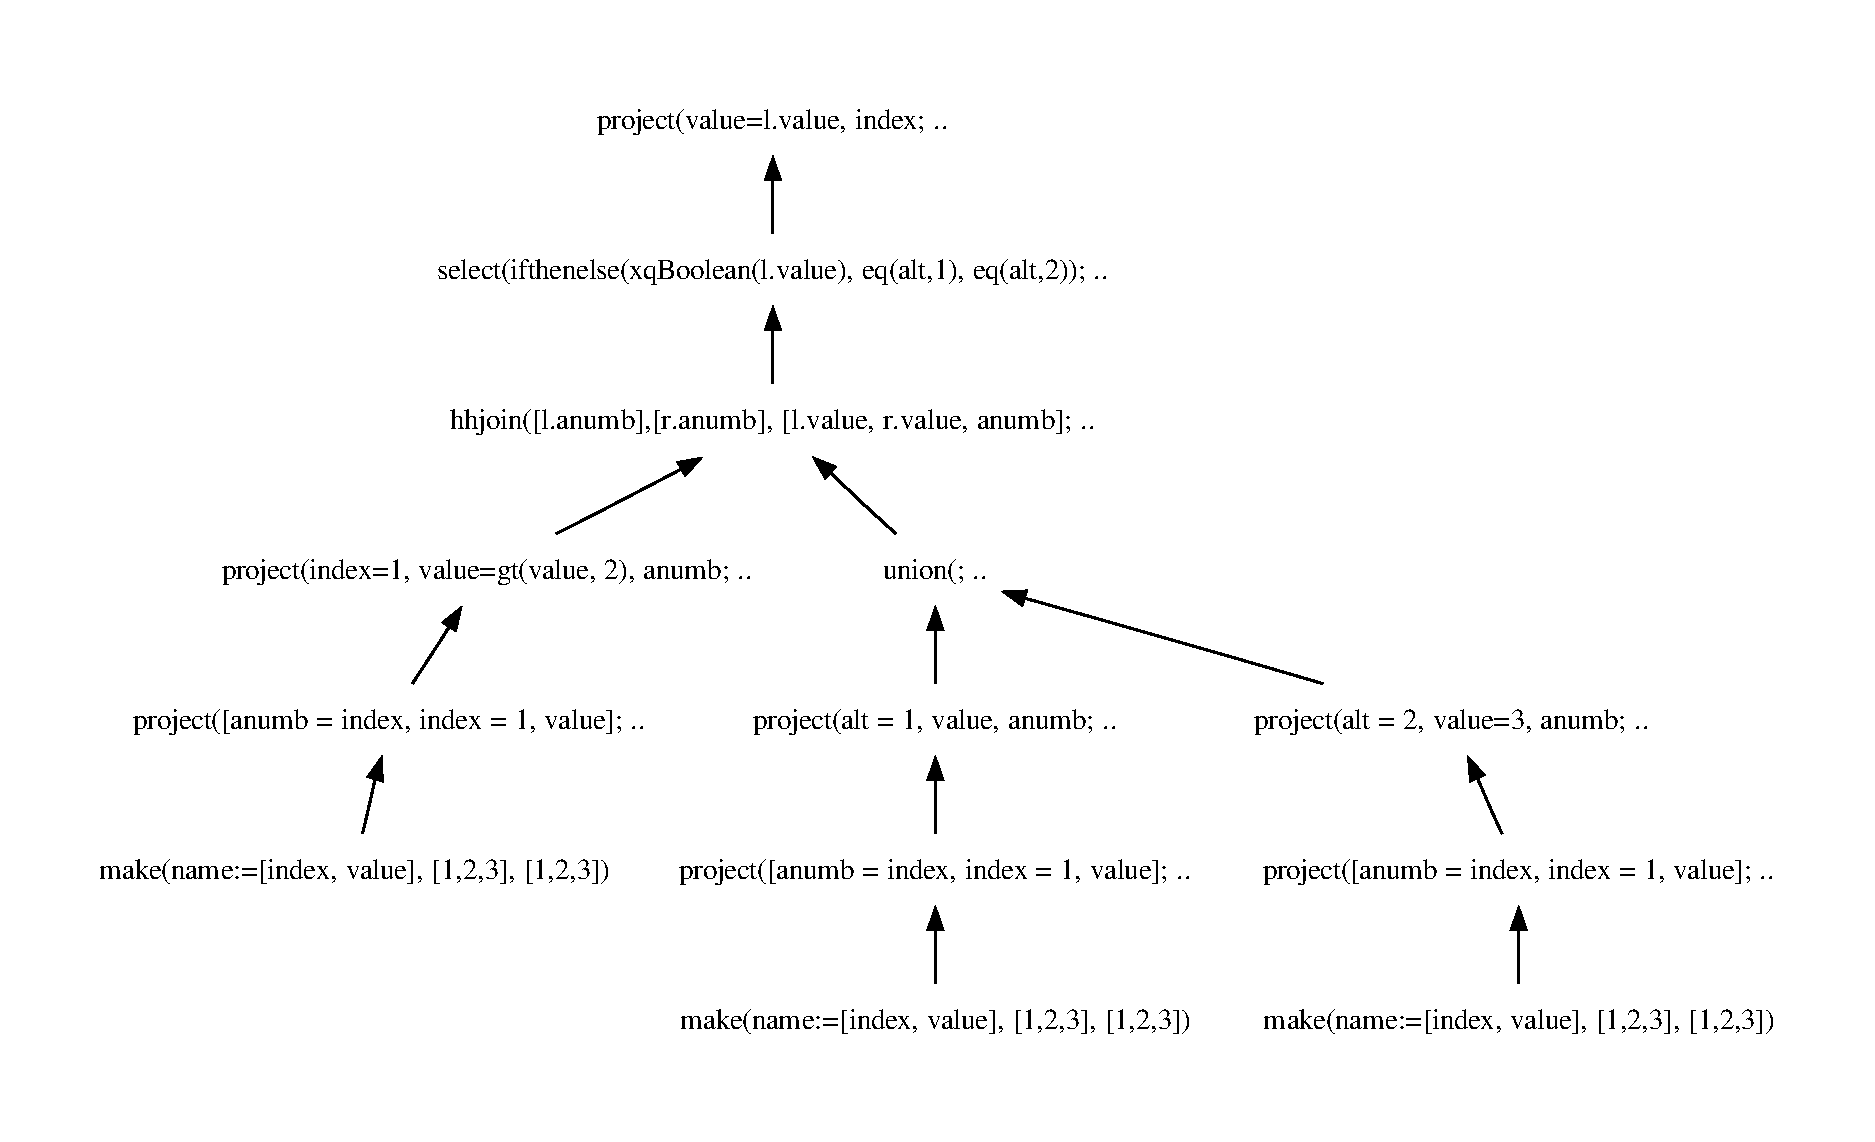
\includegraphics[width=1.0\textwidth]{img/graphs/ifthenelse}
  \caption{Complete translation of expression in figure
  \ref{fig:results:query_ifthenelse}}
  \label{fig:results:query_ifthenelse_result}
\end{center}
\end{figure}

The operator tree in figure \ref{fig:results:query_ifthenelse_result} can be
converted to the DAG seen in figure \ref{fig:results:query_ifthenelse_result_dag}.

\newpage

\begin{figure}[!htp]
\begin{center}
  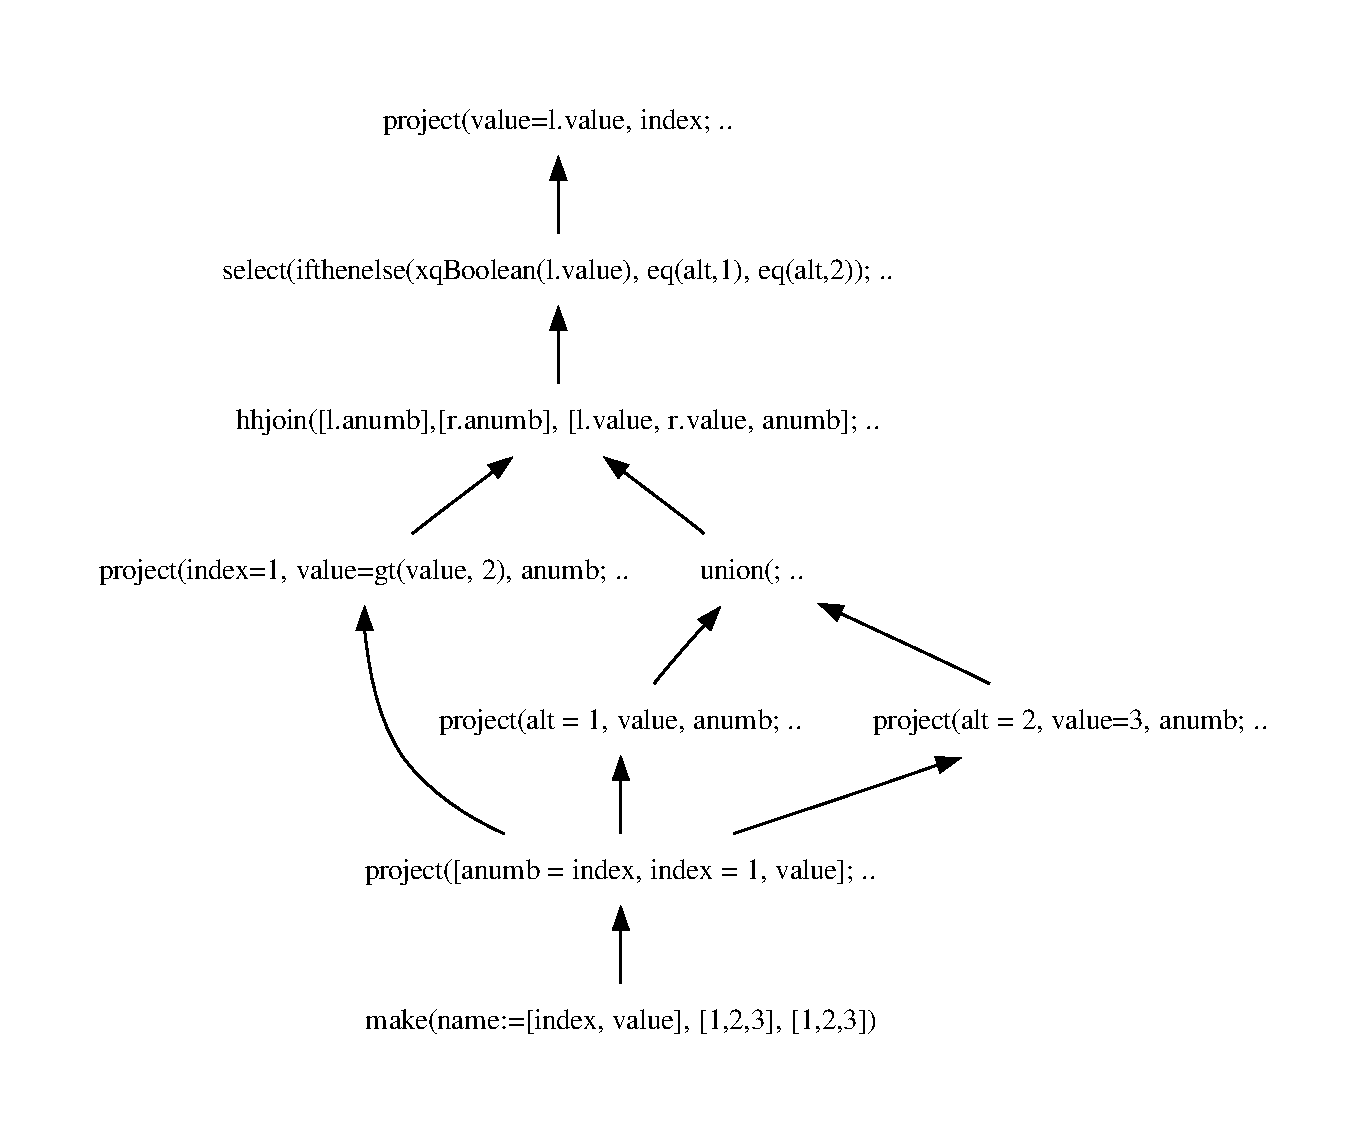
\includegraphics[width=1.0\textwidth]{img/graphs/ifthenelse_dag}
  \caption{DAG representation of operator tree in figure
  \ref{fig:results:query_ifthenelse_result}}
  \label{fig:results:query_ifthenelse_result_dag}
\end{center}
\end{figure}

\newpage

\section{Algebra Generated By Implementation}
\label{sect:result:implementation_algebra}
In this section, a collection of trivial queries are translated to relational
algebra using the implemented proof of concept described in chapter
\ref{chapter:implementation}. Naturally, this implementation also uses the
``Tainting Dependencies'' method, however the results from these translations
can also be used in a comparison with loop lifting.

\subsection{Trivial FLWOR}
\label{sect:results:algebra:generated:trivial_flwor}
\subsubsection{Query premise}
\begin{figure}[!htp]
\begin{center}
\begin{Verbatim}
for $a in (1,2,3) return $a
\end{Verbatim}
  \caption{Trivial FLWOR query premise}
  \label{fig:results:query_trivial_flwor}
\end{center}
\end{figure}

\subsubsection{Result}
\begin{figure}[!htp]
\begin{center}
  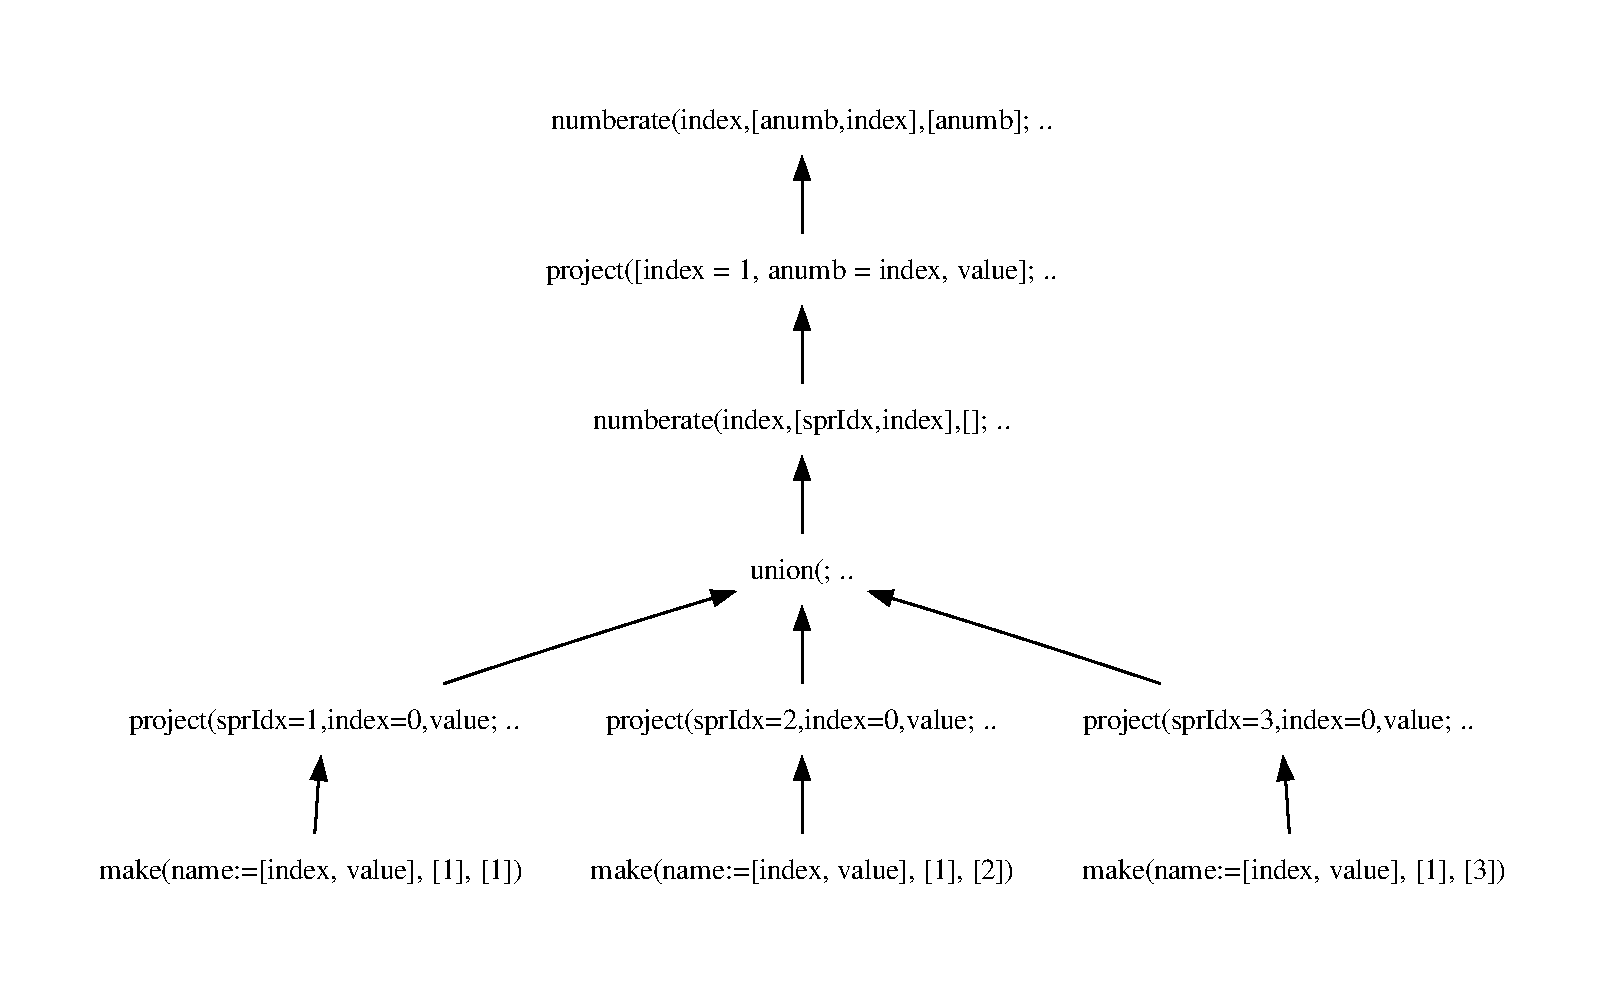
\includegraphics[width=1.0\textwidth]{img/graphs/td_impl_flwor_simple_xq_relalg} \caption{Complete translation of expression in figure
  \ref{fig:results:query_trivial_flwor}}
  \label{fig:results:query_trivial_flwor_result}
\end{center}
\end{figure}

\subsection{Complex FLWOR}
\label{sect:results:algebra:generated:complex_flwor}
\subsubsection{Query premise}
\begin{figure}[!htp]
\begin{center}
\begin{Verbatim}
for $a in (1,2) return (3, for $b in (4,5) return ($a, $b, 6))
\end{Verbatim}
  \caption{Complex FLWOR query premise}
  \label{fig:results:query_complex_flwor}
\end{center}
\end{figure}

\subsubsection{Result}
\begin{figure}[!htp]
\begin{center}
  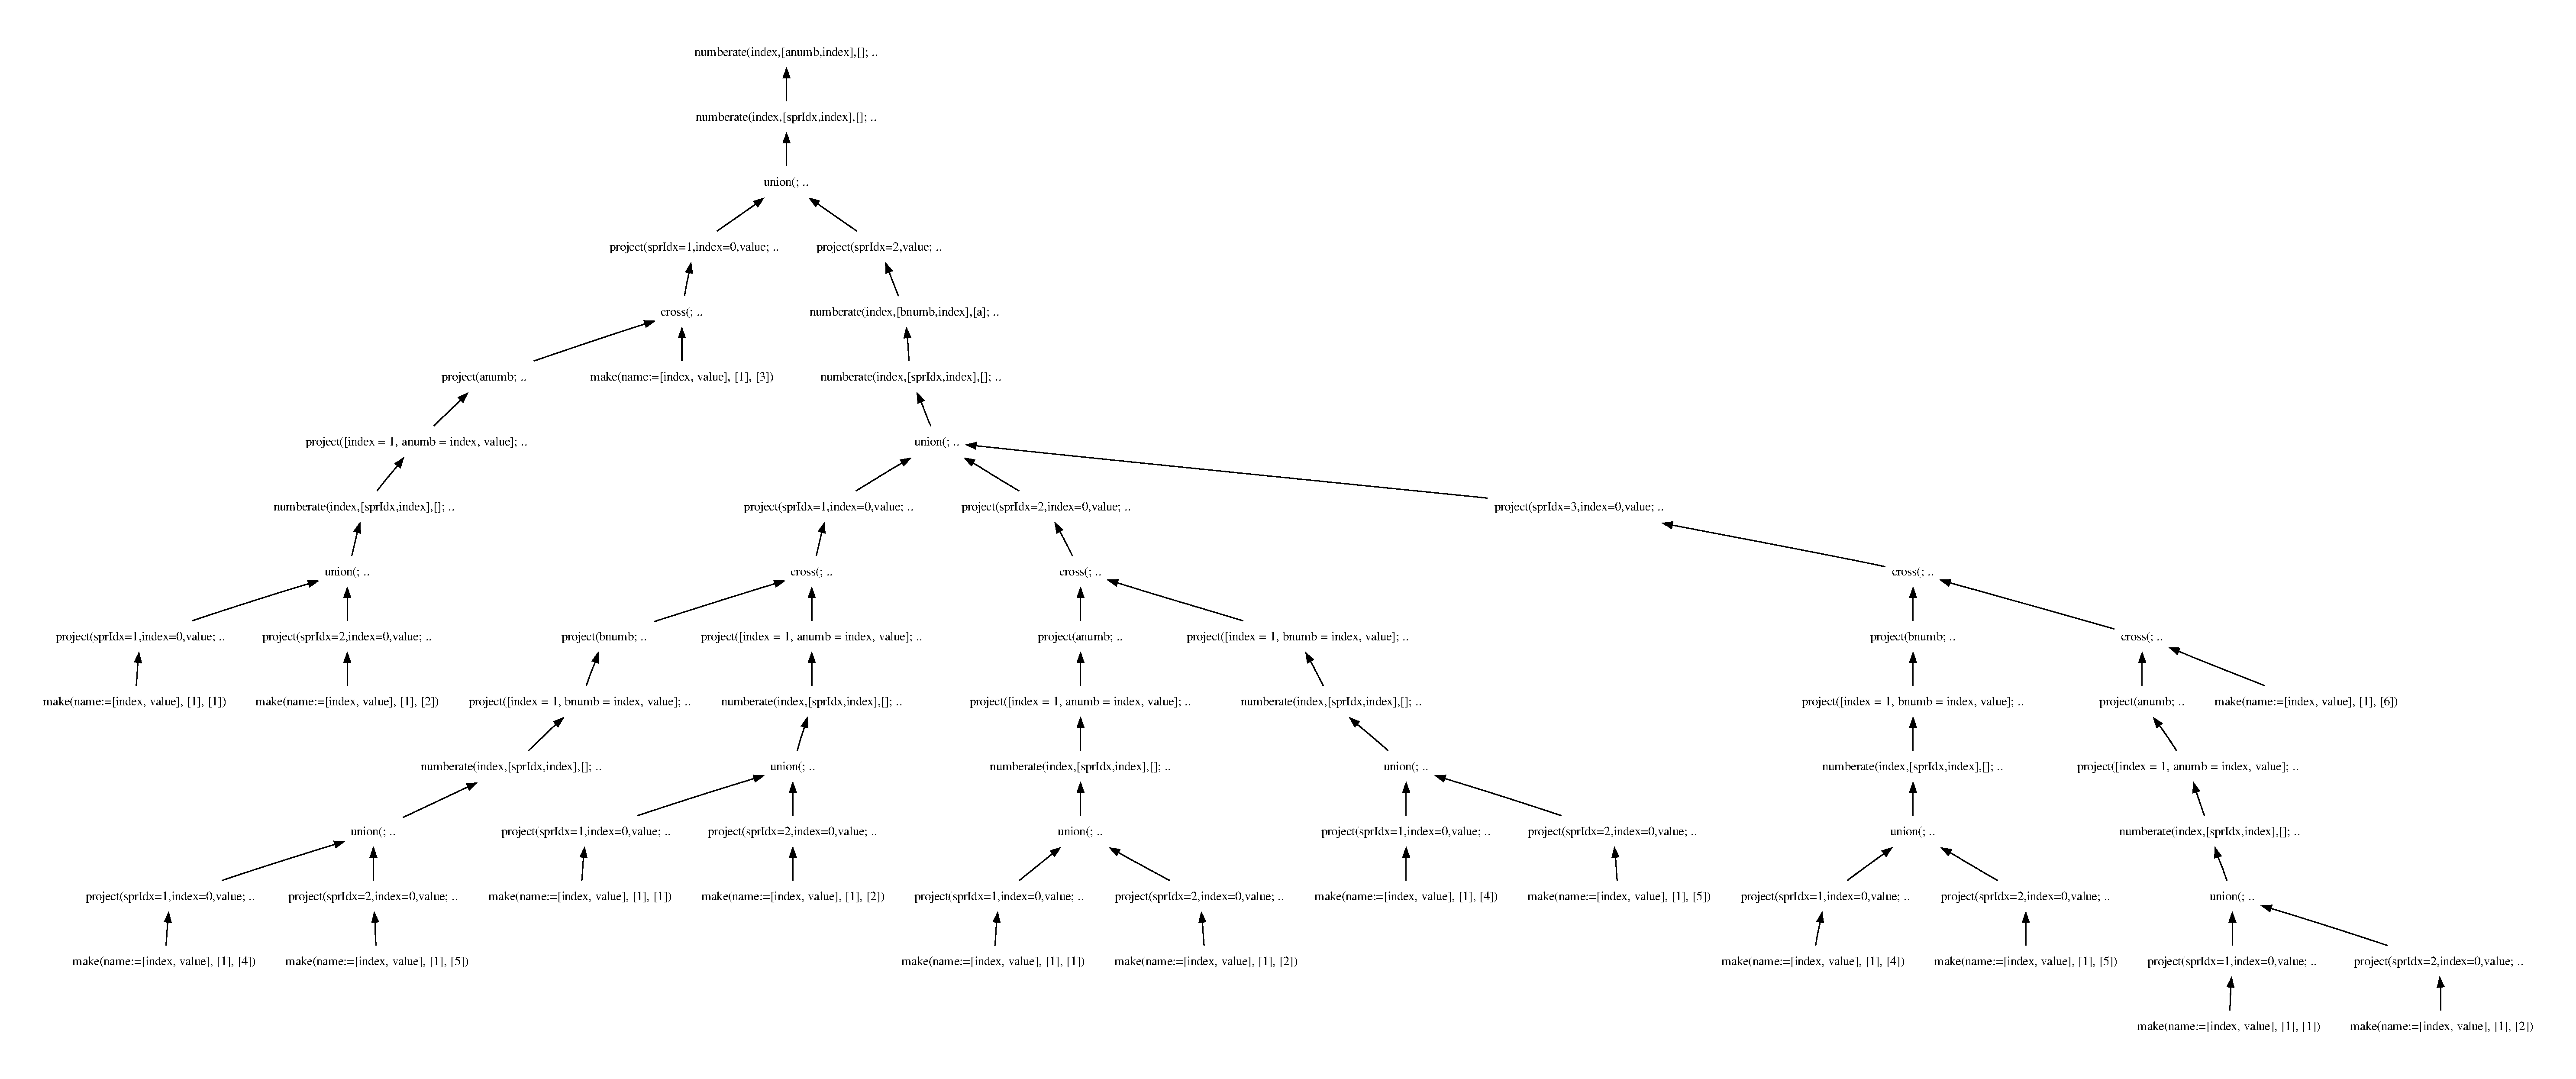
\includegraphics[angle=90,height=0.7\textheight]{img/graphs/td_impl_flwor_complex_xq_relalg} \caption{Complete
  translation of expression in figure
  \ref{fig:results:query_complex_flwor}}
  \label{fig:results:query_complex_flwor_result}
\end{center}
\end{figure}


The algebra tree in figure \ref{fig:results:query_complex_flwor_result} can
be converted to the DAG in figure
\ref{fig:results:query_complex_flwor_result_dag}

\begin{figure}[!htp]
\begin{center}
  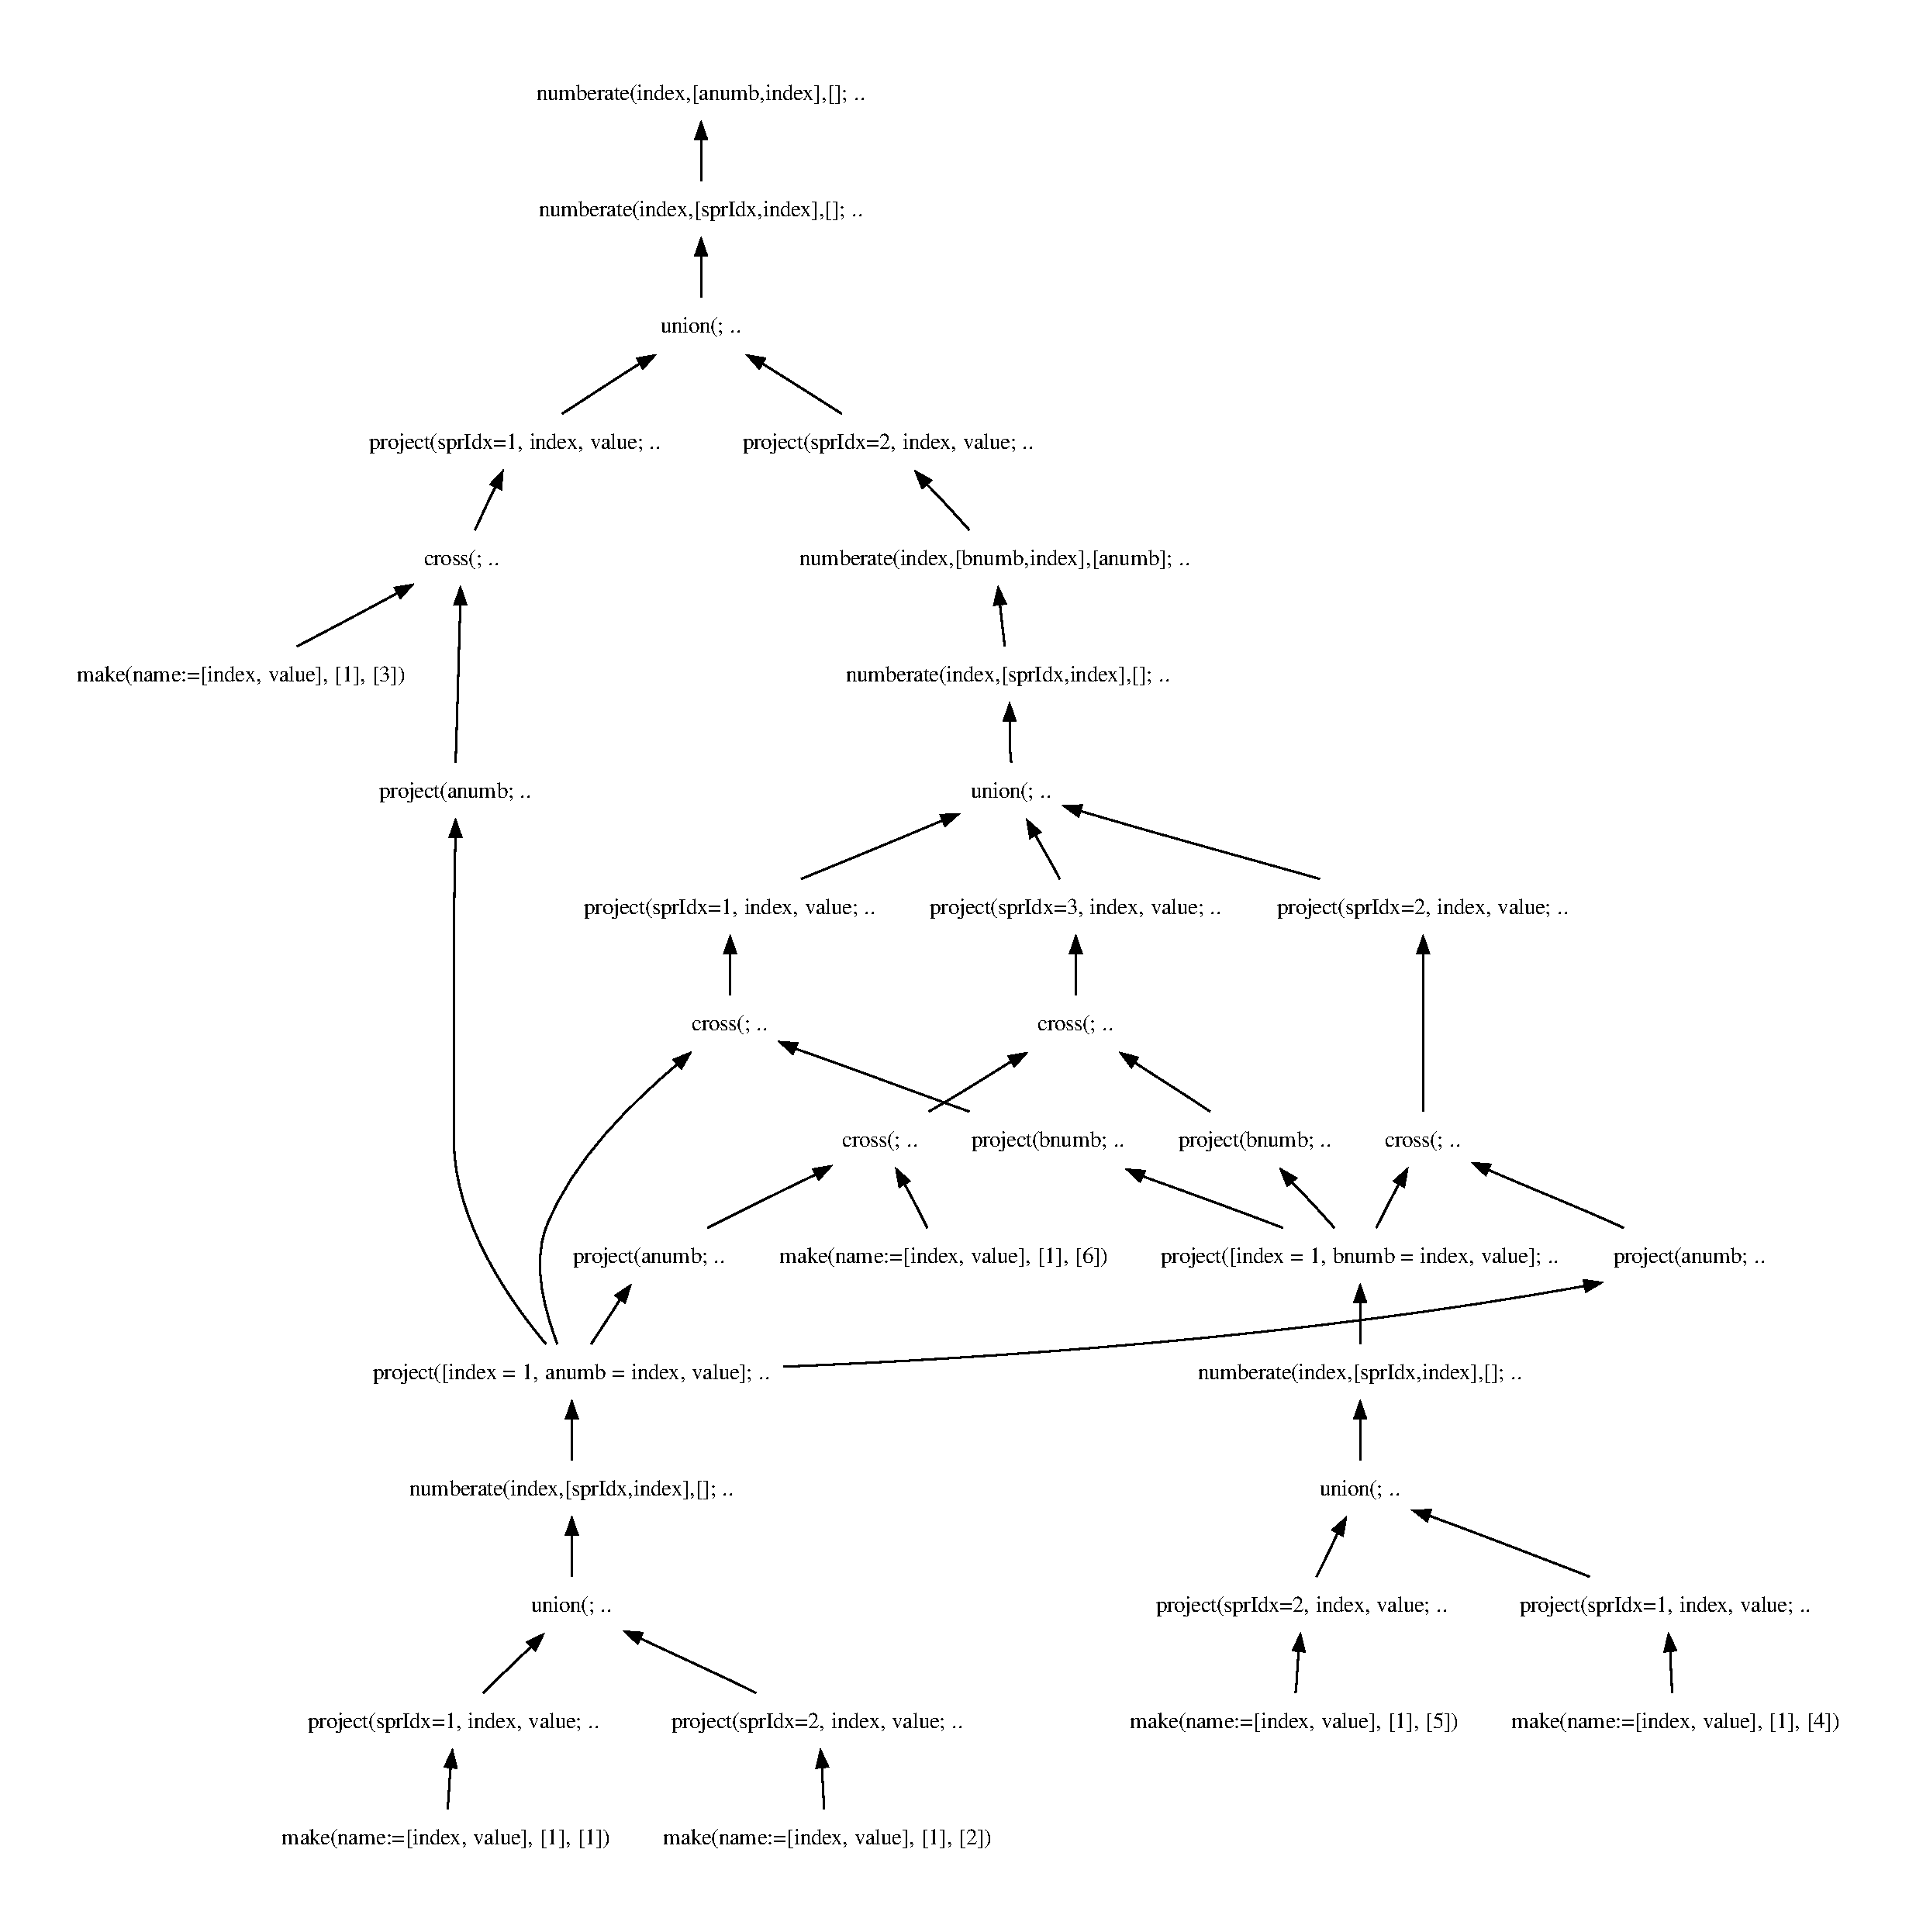
\includegraphics[width=1.0\textwidth]{img/graphs/td_impl_flwor_complex_xq_relalg_dag}
  \caption{Complete translation of expression in figure
  \ref{fig:results:query_complex_flwor} converted to a DAG}
  \label{fig:results:query_complex_flwor_result_dag}
\end{center}
\end{figure}
\newpage

\subsection{FLWOR with conditional}
\label{sect:results:algebra:generated:conditional_flwor}
\subsubsection{Query premise}
\begin{figure}[!htp]
\begin{center}
\begin{Verbatim}
for $a in (10,20) return if ($a > 15) then $a else 15
\end{Verbatim}
  \caption{Conditional FLWOR query premise}
  \label{fig:results:query_conditional_flwor}
\end{center}
\end{figure}

\subsubsection{Result}
\begin{figure}[!htp]
\begin{center}
  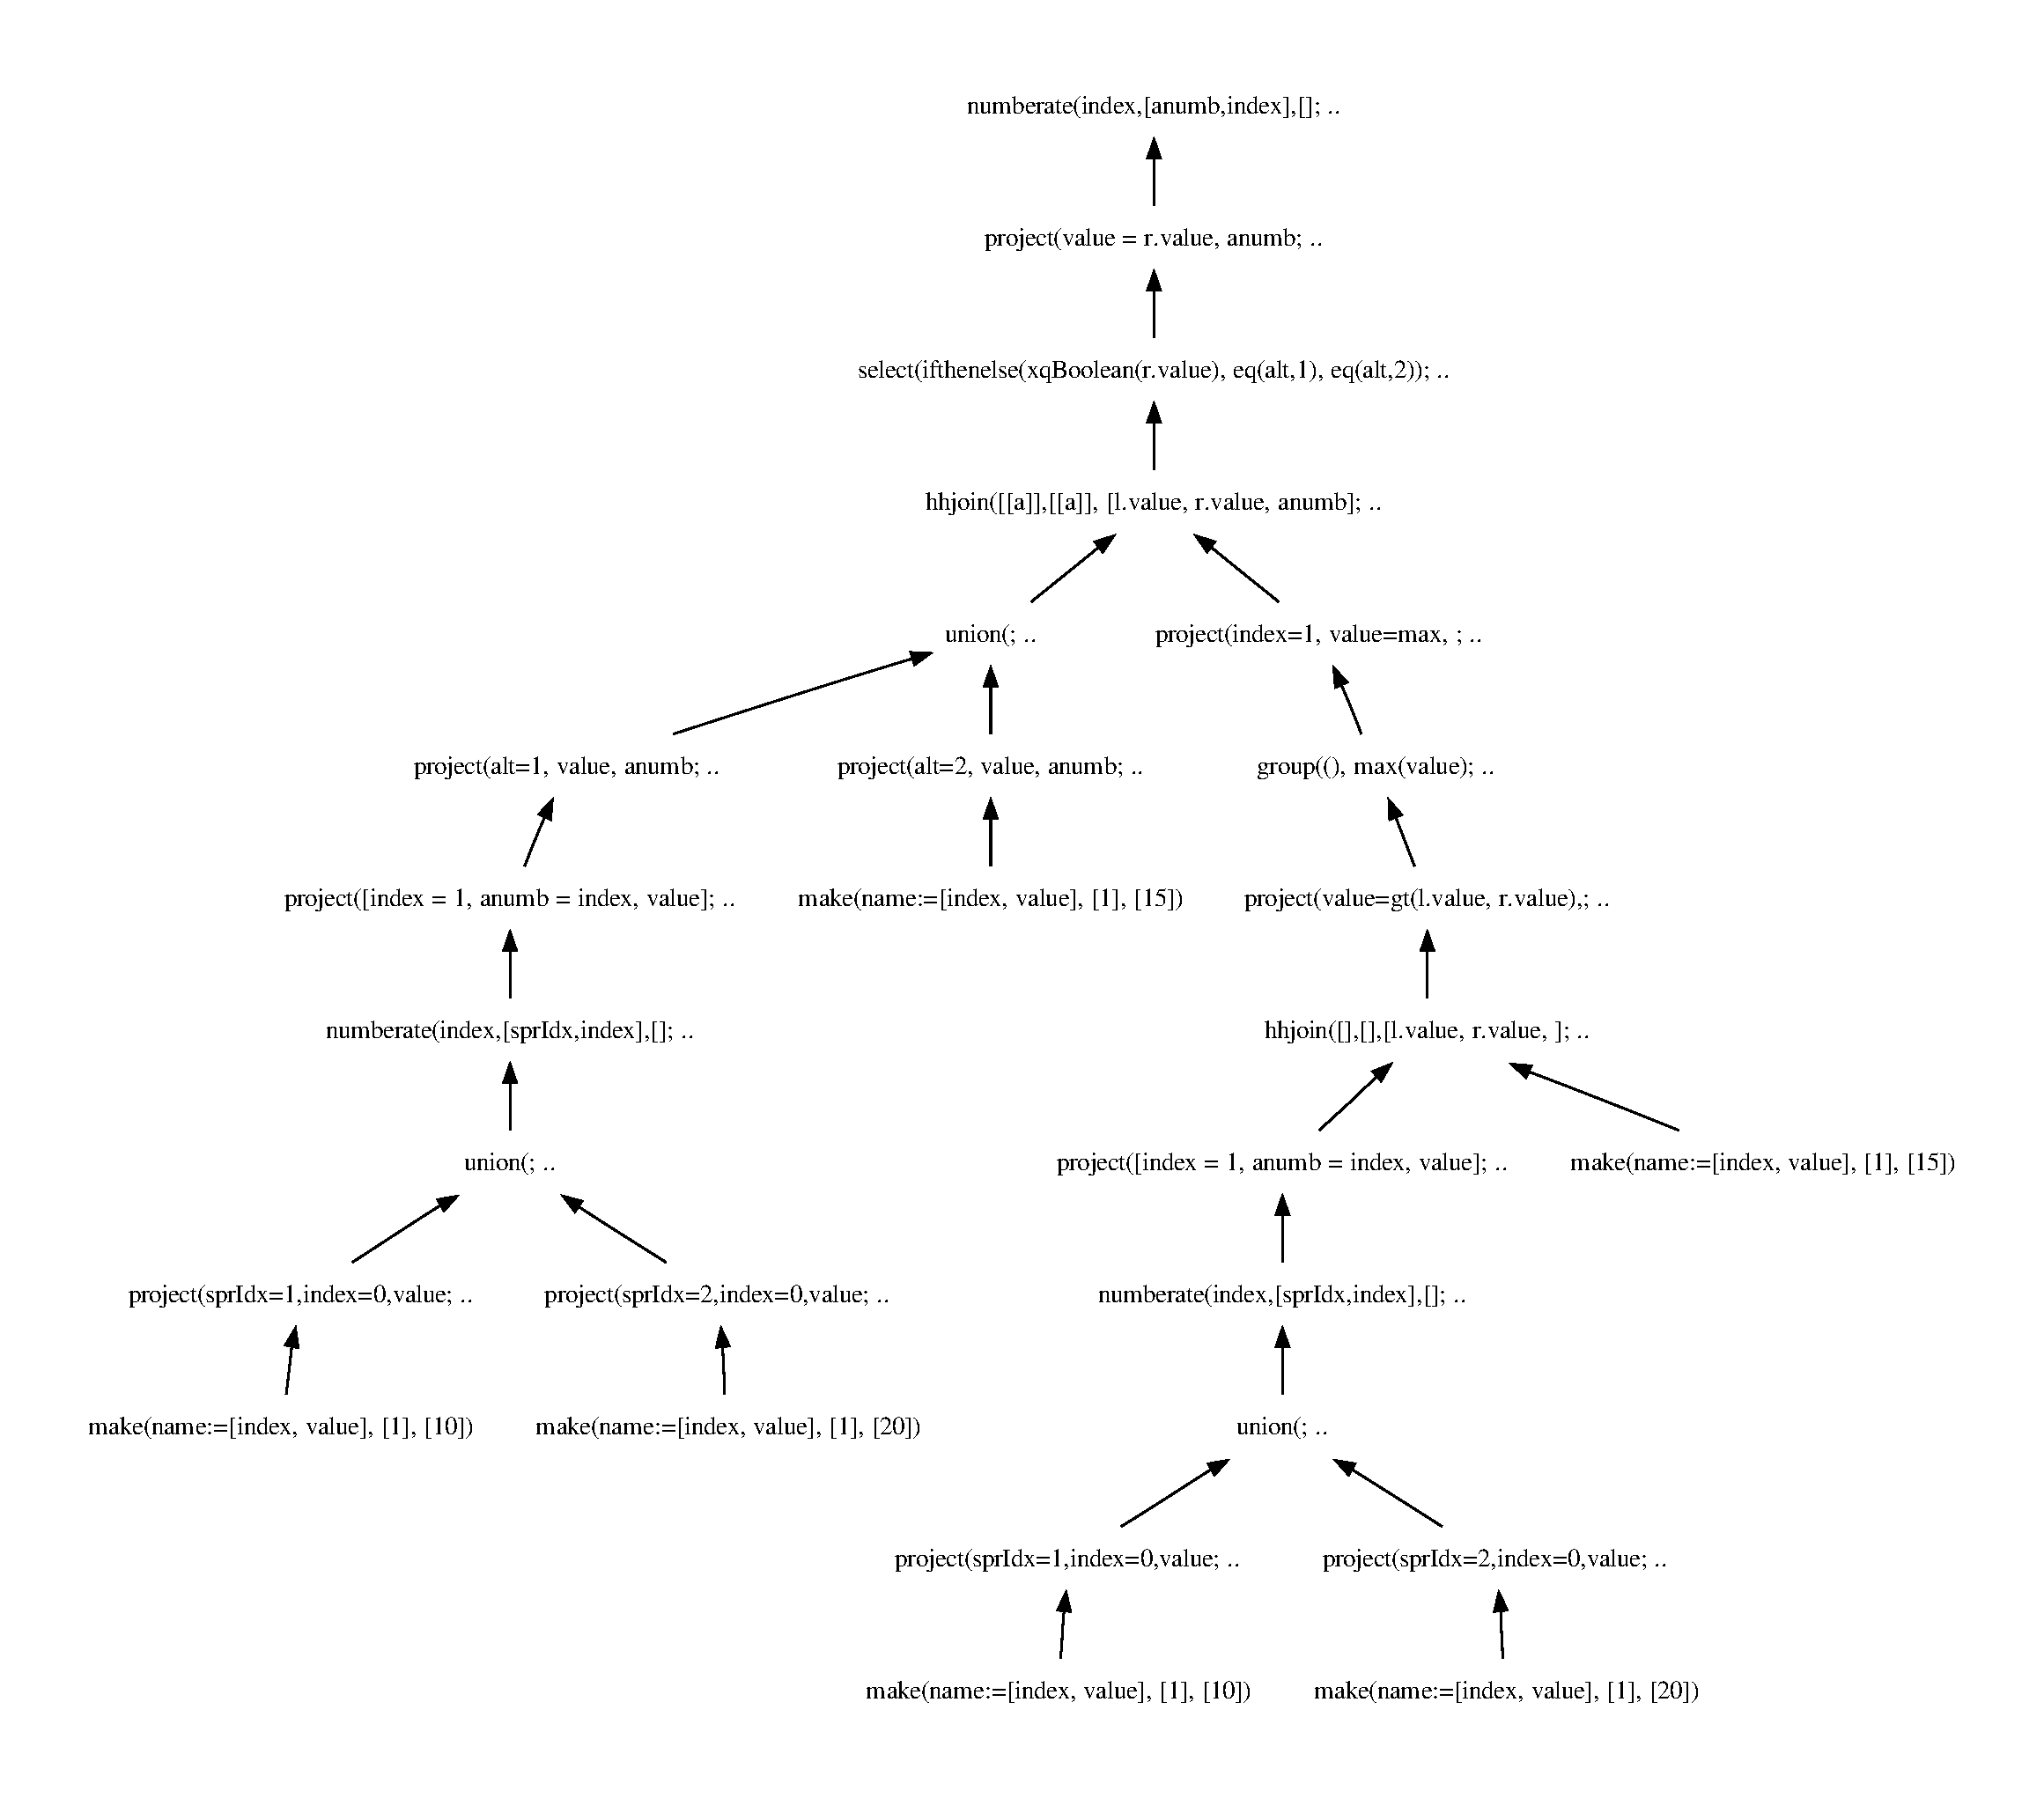
\includegraphics[width=1.0\textwidth]{img/graphs/td_impl_flwor_ifthenelse_xq_relalg}
  \caption{Complete translation of expression in figure
  \ref{fig:results:query_conditional_flwor}}
  \label{fig:results:query_conditional_flwor_result}
\end{center}
\end{figure}

The algebra tree in figure \ref{fig:results:query_conditional_flwor_result} can
be converted to the DAG in figure
\ref{fig:results:query_conditional_flwor_result_dag}

\newpage
\begin{figure}[!htp]
\begin{center} 
  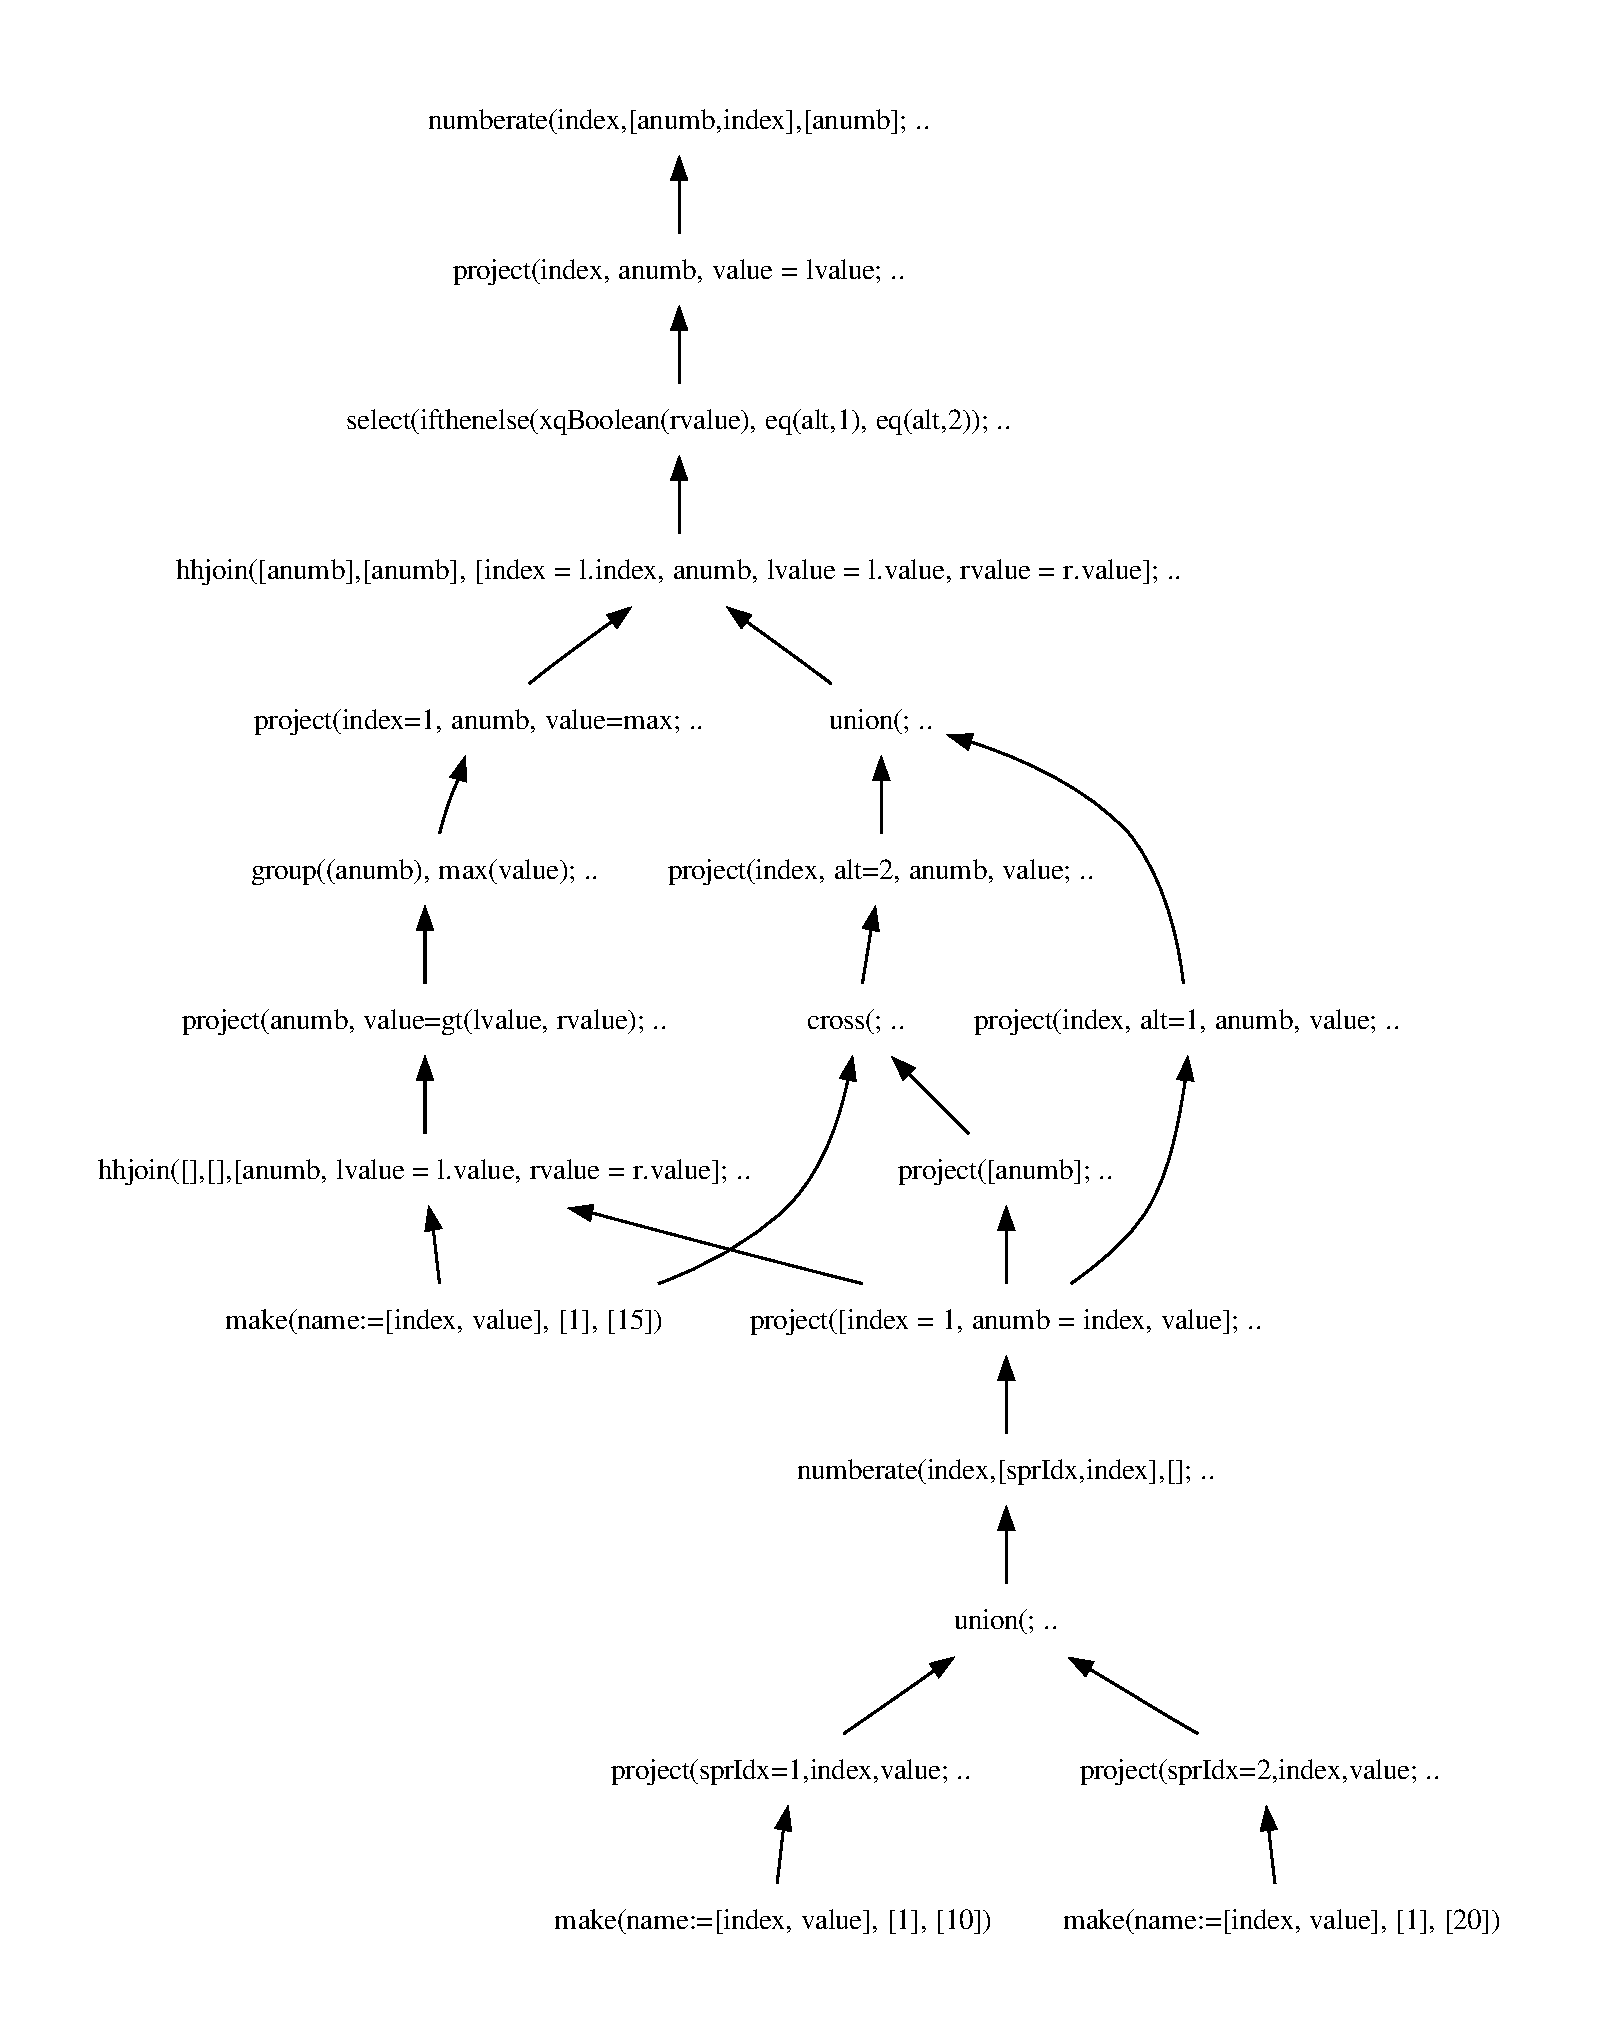
\includegraphics[width=1.0\textwidth]{img/graphs/td_impl_flwor_ifthenelse_xq_relalg_dag}
  \caption{Complete translation of expression in figure
  \ref{fig:results:query_conditional_flwor} converted to a DAG}
  \label{fig:results:query_conditional_flwor_result_dag}
\end{center}
\end{figure}
\section{Comparison}
\label{sect:results:comparison}
\subsection{Assumptions}
This comparison must be seen in the context of a number of assumptions
about the systems being compared. With regards to fairness, it is important to
note that the algebra trees generated by Pathfinder may have been
optimised (to which the exact extent is not known), while the algebra trees
generated by the prototype developed throughout this project \emph{does not apply any optimalisations} at all. The
optimalisations applied by Pathfinder are noted
in \cite{pathfinder_purelyRelational}.

Some important effects on the Pathfinder algebra tree from these
optimalisations are:
\begin{itemize}
  \item The cartesian products between a loop relation and a constant
  subexpression are transformed into projections
  \item The custom operator \textsf{attach} is roughly a simpler equivalent to
  the \textsf{make()} operator in MQL (see section \ref{sect:method:mql}, page
  \pageref{sect:method:mql})
\end{itemize}
TODO: noe mer her?

\newpage
\subsection{DAG comparison}
Note that the readability for these DAG comparisons are not essential --
however, links to large-scale versions of these diagrams are noted in appendix
\ref{appendix:links_and_resources}.

\begin{figure}[!h]
	\centering
	\mbox{
		\subfigure[Pathfinder/MonetDB]{		
			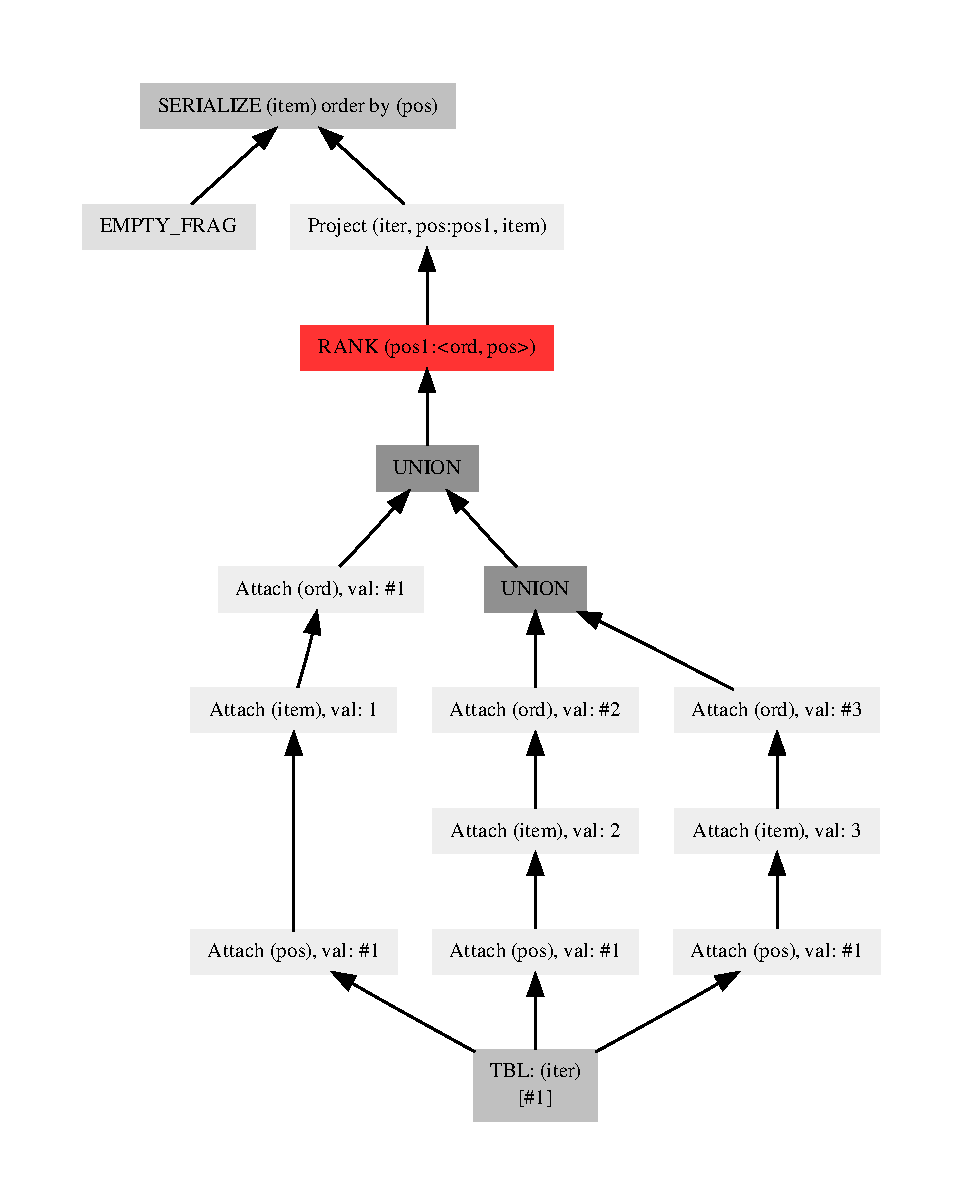
\includegraphics[width=0.4\textwidth]{img/graphs/td_impl_flwor_simple_pathfinder}
			\label{fig:result:comparison:simple_dag}
		}
		\quad
		\subfigure[Prototype implementation]{
		
			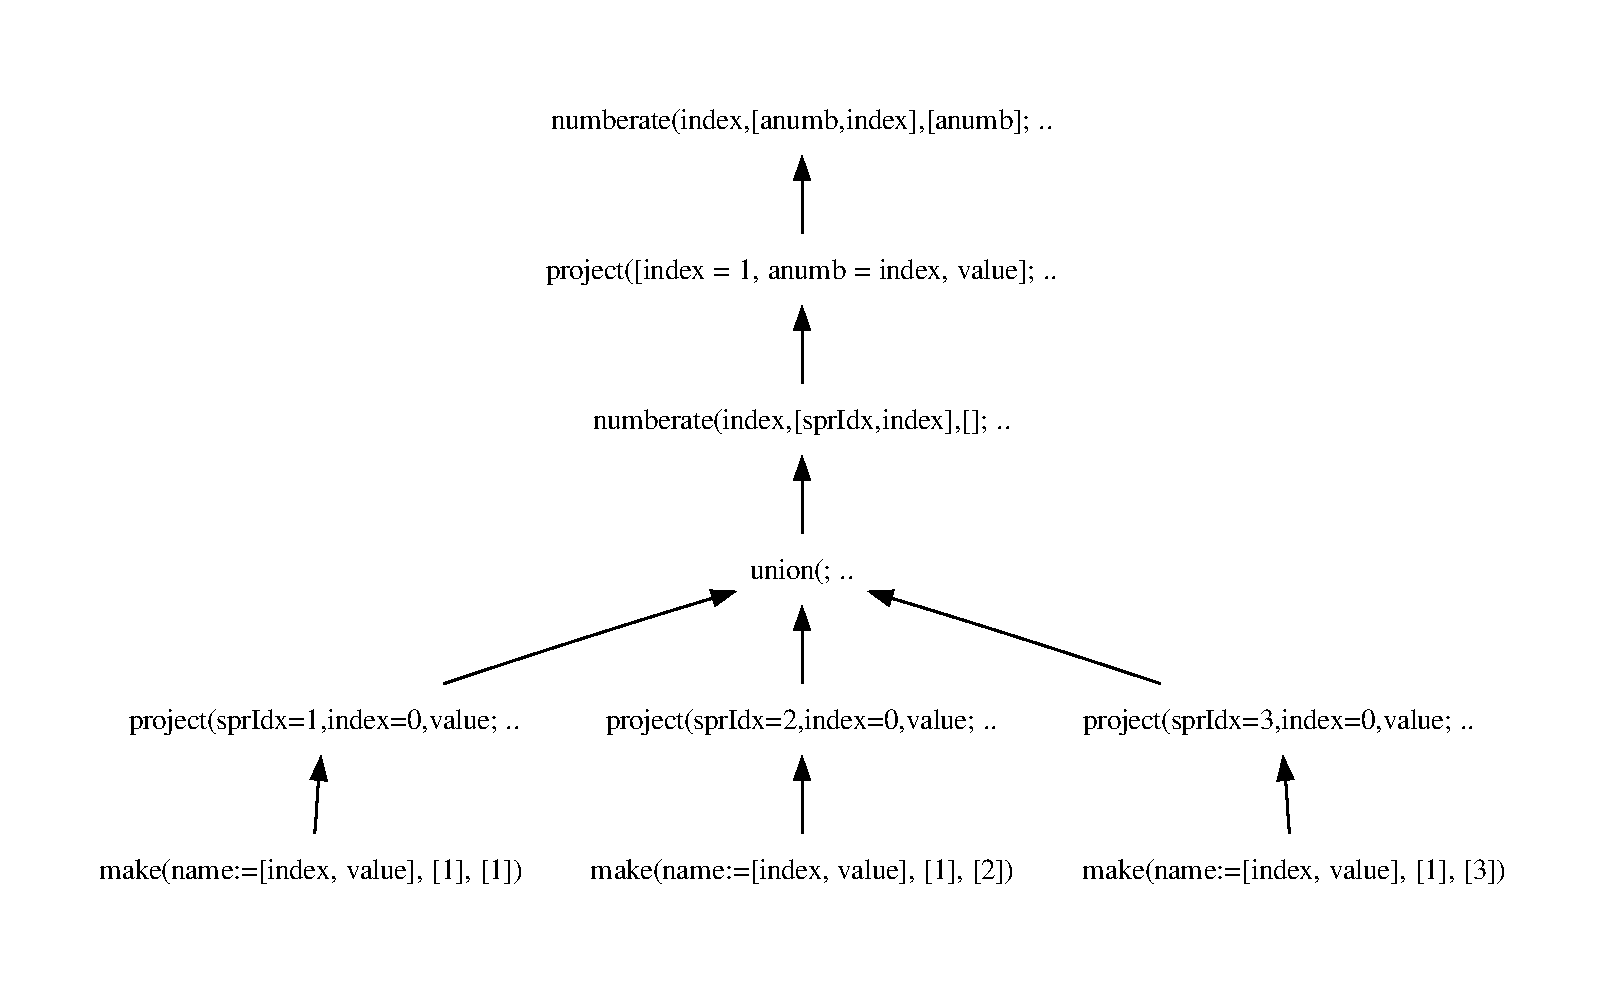
\includegraphics[width=0.6\textwidth]{img/graphs/td_impl_flwor_simple_xq_relalg}
			\label{fig:result:comparison:simple_pathfinder_dag}
		}
	}
	\caption{Comparison of DAGs for the trivial expression in section
	\ref{sect:results:algebra:generated:trivial_flwor}}
\end{figure}

\newpage
\begin{figure}[!h]
	\centering
	\mbox{
		\subfigure[Pathfinder/MonetDB]{		
			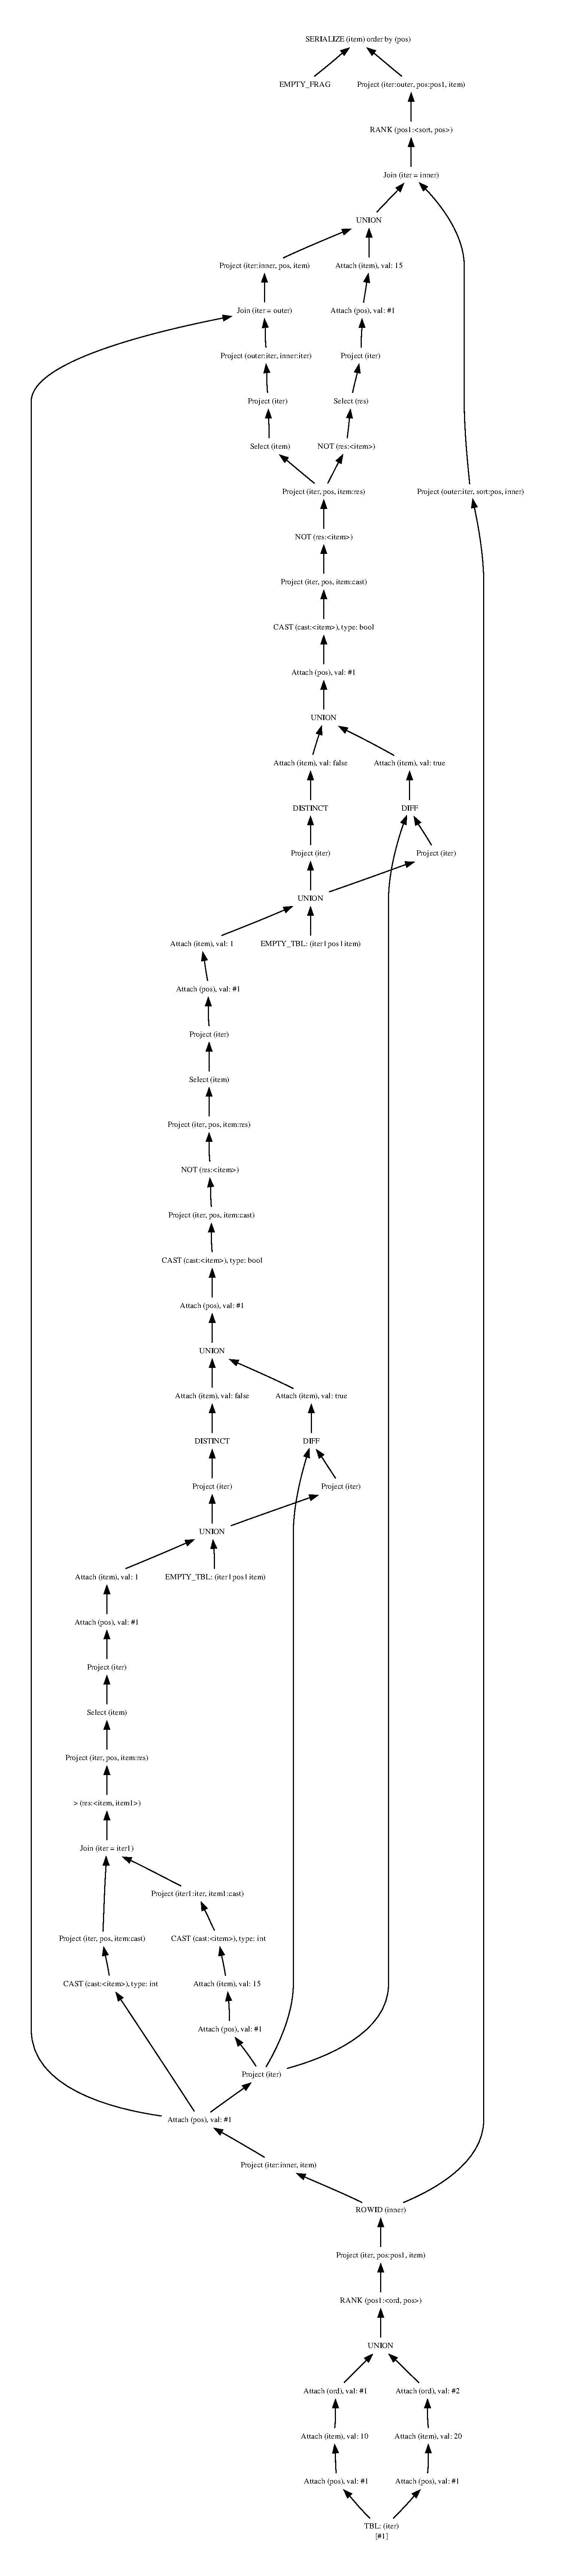
\includegraphics[width=0.3\textwidth]{img/graphs/td_impl_flwor_ifthenelse_pathfinder}
			\label{fig:result:comparison:conditional_dag}
		}
		\quad
		\subfigure[Prototype implementation]{
		
			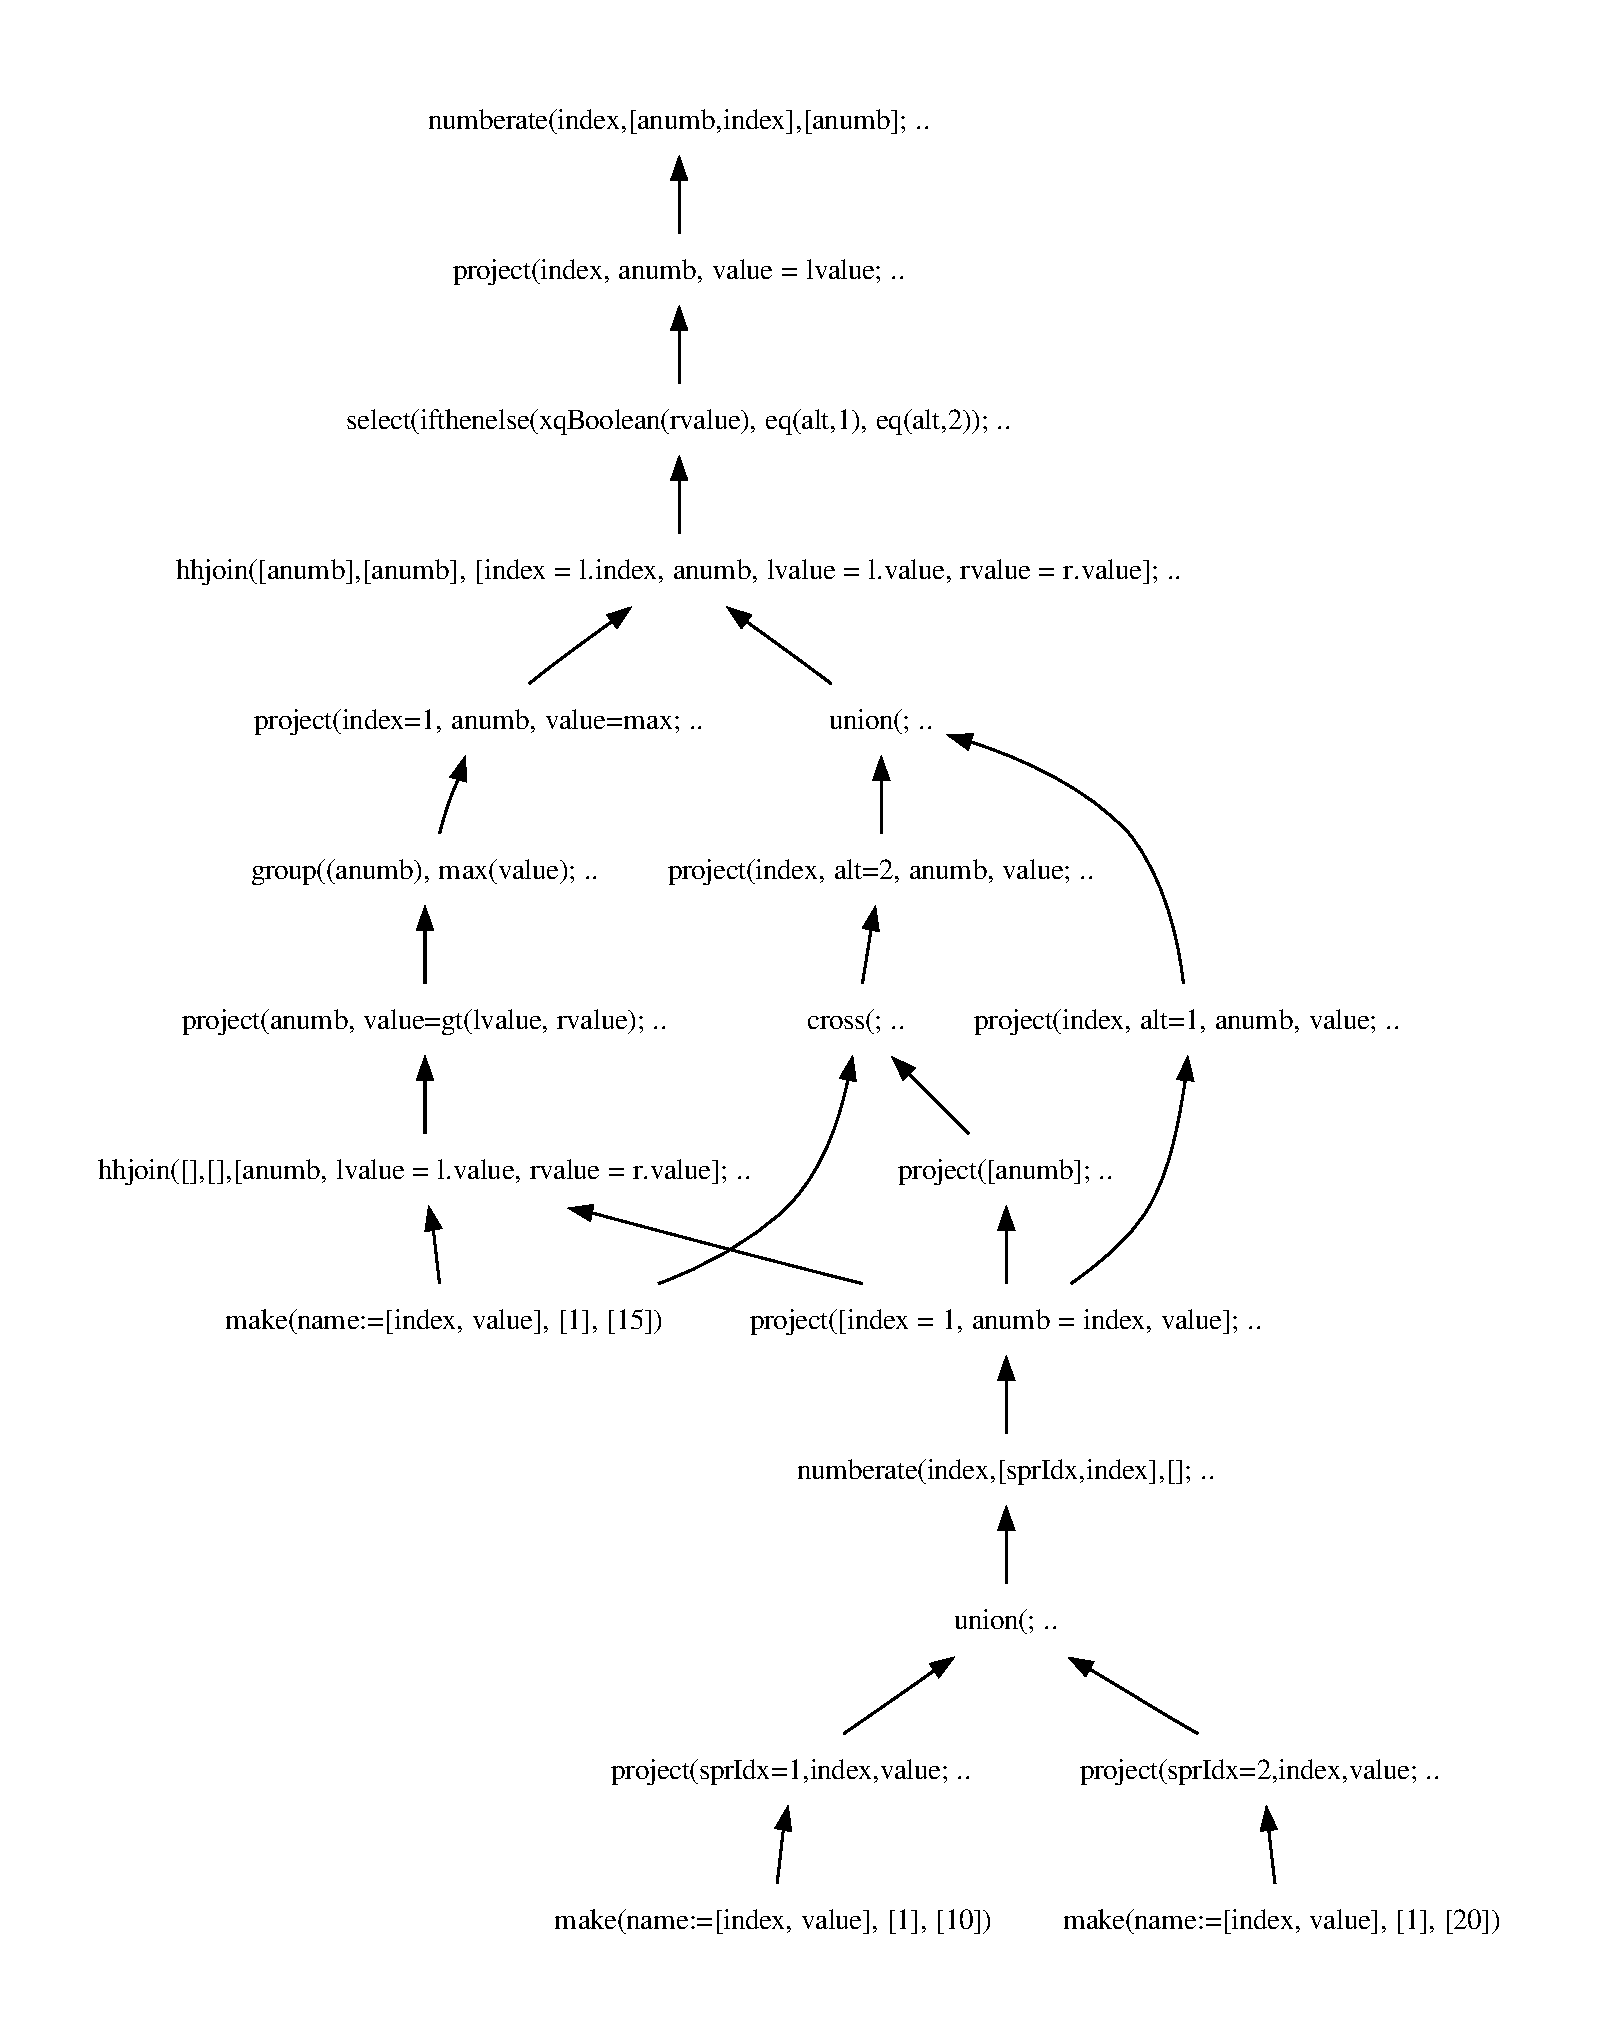
\includegraphics[width=0.7\textwidth]{img/graphs/td_impl_flwor_ifthenelse_xq_relalg_dag}
			\label{fig:result:comparison:conditional_pathfinder_dag}
		}
	}
	\caption{Comparison of DAGs for the conditional expression in section
	\ref{sect:results:algebra:generated:conditional_flwor}}
\end{figure}

\newpage
\begin{figure}[!h]
	\centering
	\mbox{
		\subfigure[Pathfinder/MonetDB]{		
			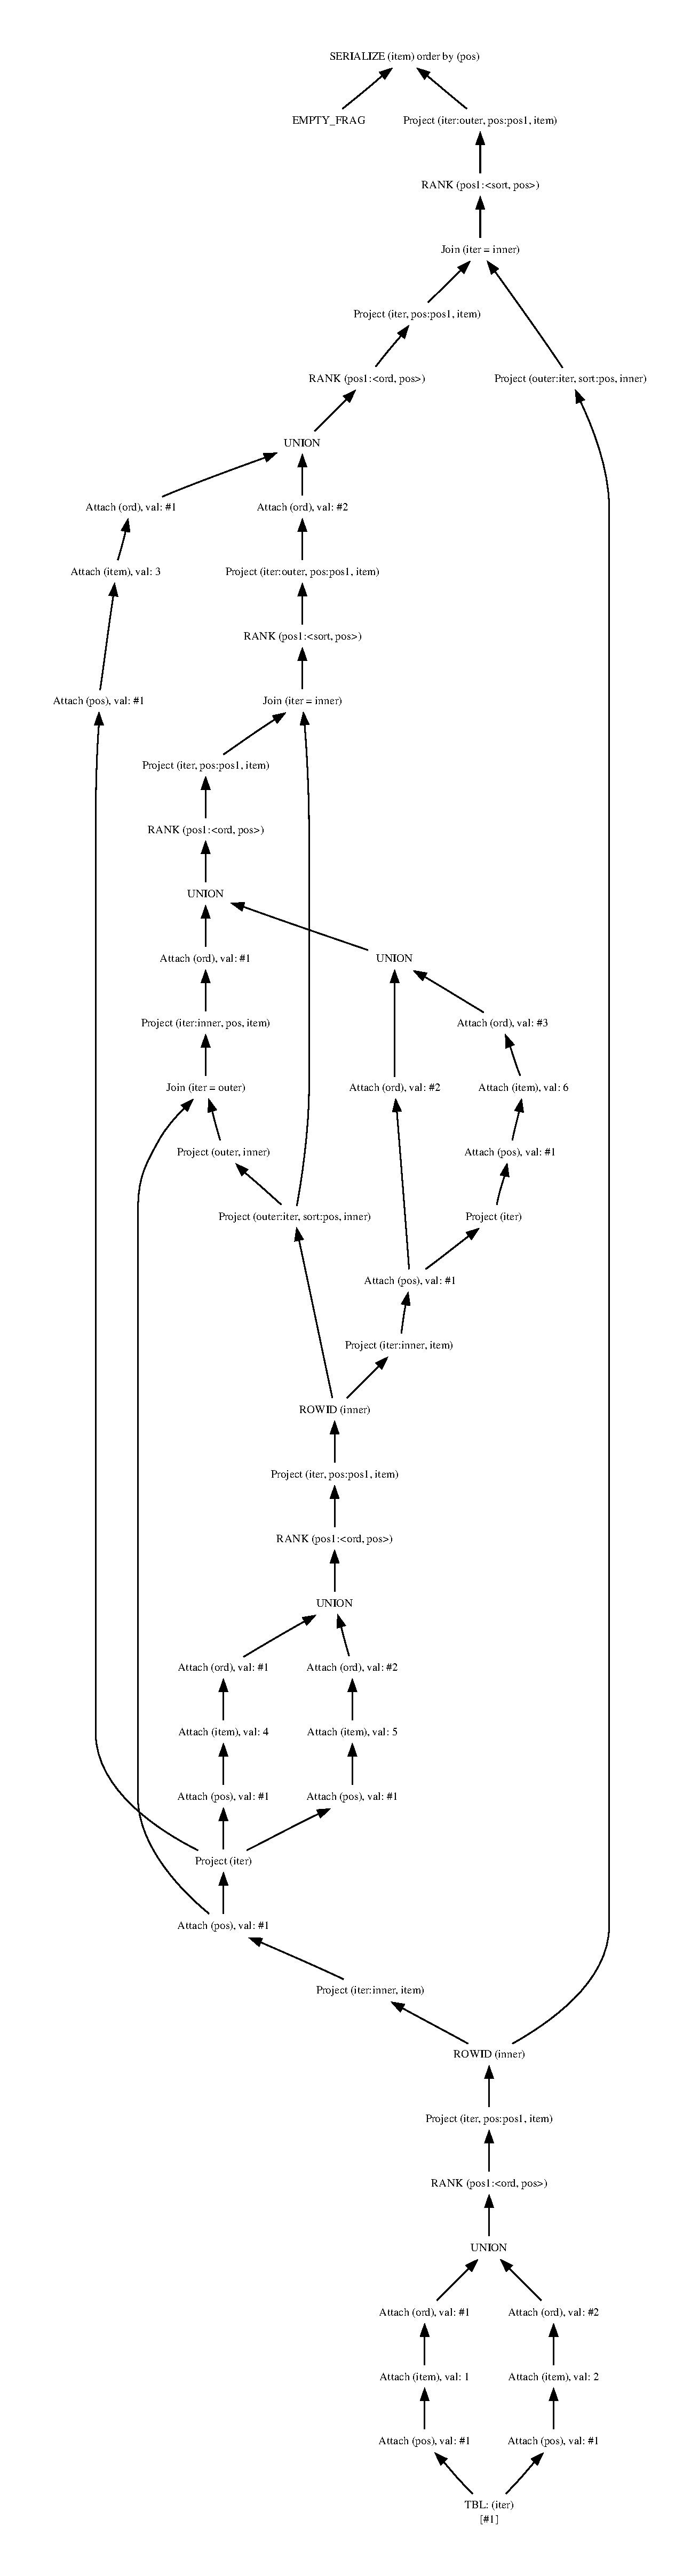
\includegraphics[width=0.37\textwidth]{img/graphs/td_impl_flwor_complex_pathfinder}
			\label{fig:result:comparison:complex_xqft_dag}
		}
		\quad
		\subfigure[Prototype implementation]{
		
			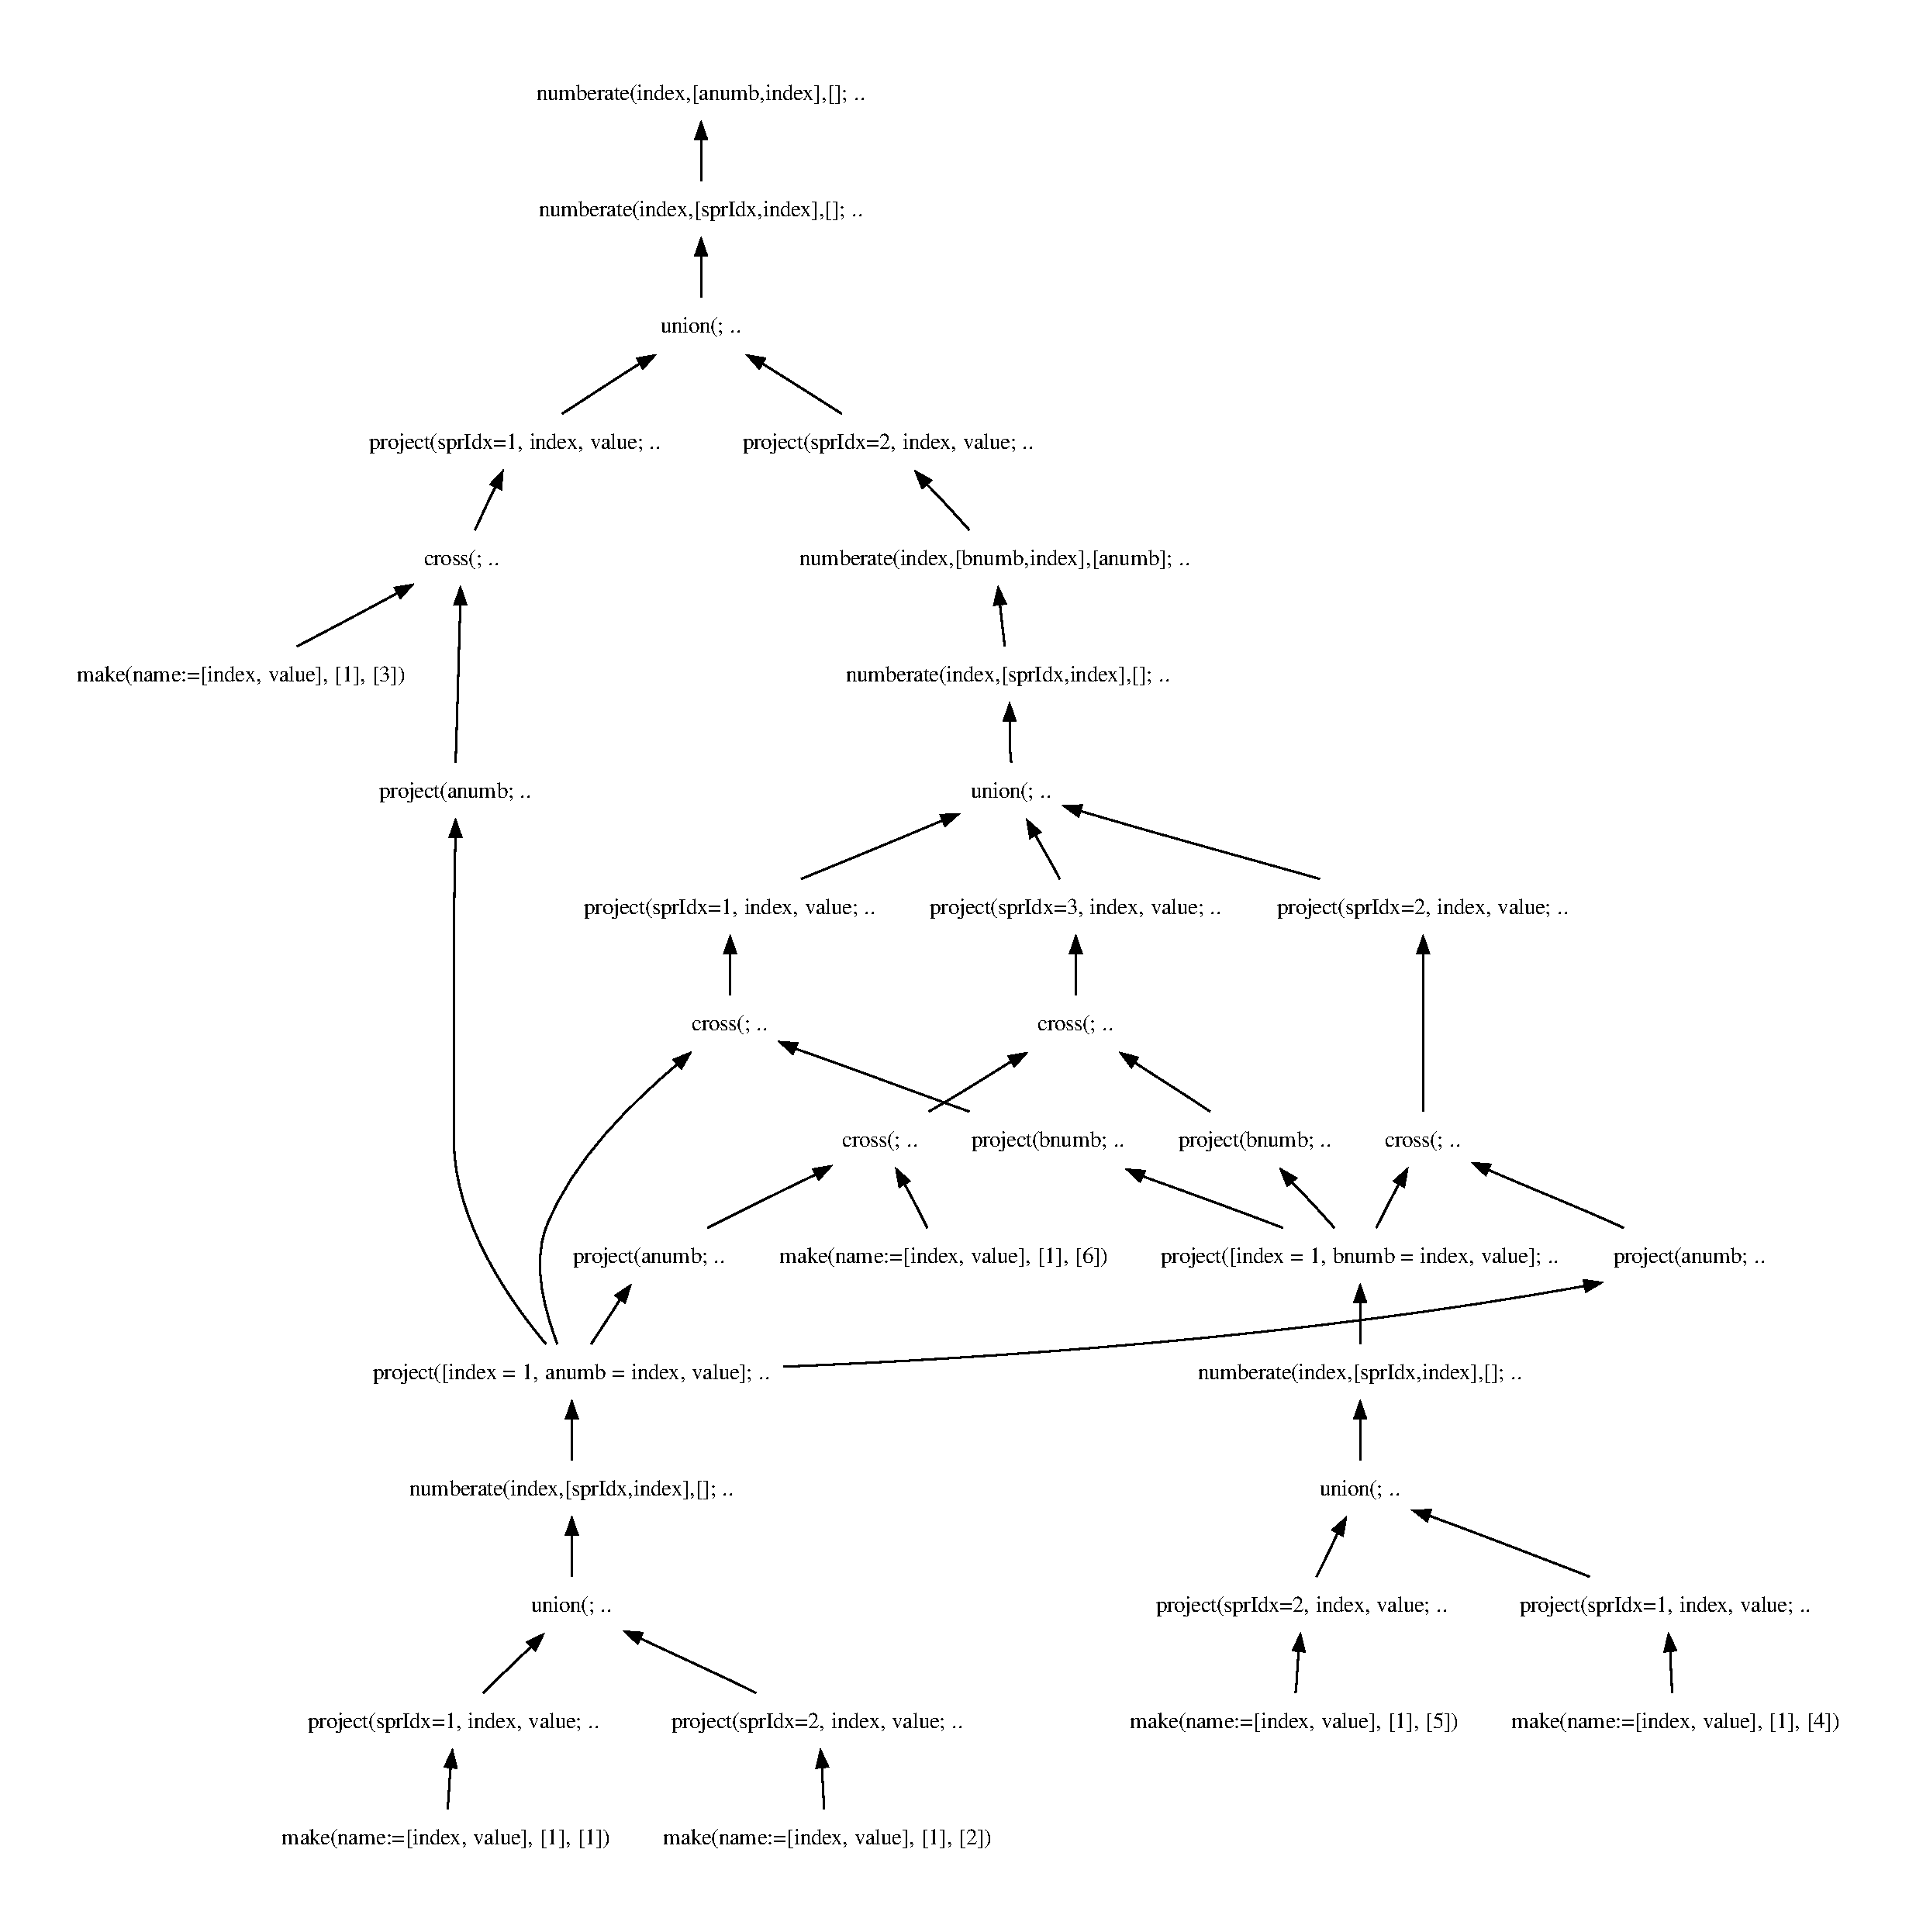
\includegraphics[width=0.6\textwidth]{img/graphs/td_impl_flwor_complex_xq_relalg_dag}
			\label{fig:result:comparison:complex_pathfinder_dag}
		}
	}
	\caption{Comparison of DAGs for the complex expression in section
	\ref{sect:results:algebra:generated:complex_flwor}}
\end{figure}

\newpage
\subsection{Complexity estimation and comparison}
Complexity estimation is performed as detailed in section
\ref{sect:method:complexity}. The complexity
comparison matrix is shown in table \ref{table:result:complexity_matrix}.

\begin{table}[!htp]
 \begin{center} 
 \begin{tabular}{| c | c | c || c | c |}
  \hline
   & \multicolumn{2}{|c||}{\textbf{Pathfinder/MonetDB}}
   & \multicolumn{2}{|c|}{\textbf{Prototype implementation}} \\
   \hline
   & Tuples & Fields & Tuples & Fields \\  
   \hline
   Trivial & 16 & 16 & 15 & 18 \\  
   \hline
   Complex & 215 & 265 & 136 & 102 \\
   \hline
   Conditional & 94 & 50 & 31 & 44 \\  
   \hline
 \end{tabular}
\caption{Complexity comparison matrix}
\label{table:result:complexity_matrix}
 \end{center}
\end{table}




\begin{figure}[!htp]
\begin{center}
  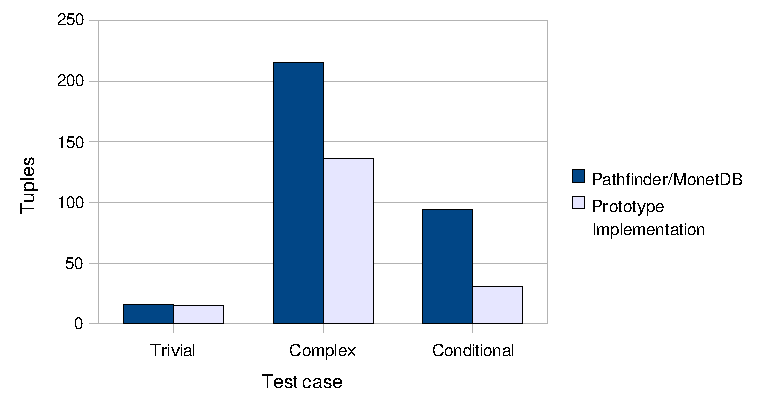
\includegraphics[width=1.0\textwidth]{diagrams/comparison_chart2_chart1}
  \caption{Comparison of complexity based on tuple creation}
  \label{fig:results:comparison:chart1}
\end{center}
\end{figure}

\begin{figure}[!htp]
\begin{center}
  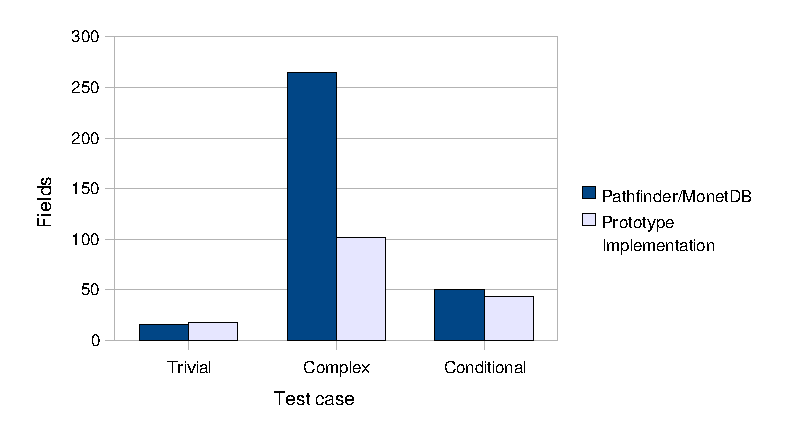
\includegraphics[width=1.0\textwidth]{diagrams/comparison_chart2_chart2}
  \caption{Comparison of complexity based on field creation}
  \label{fig:results:comparison:chart2}
\end{center}
\end{figure}

% Joins
\begin{table}[!htp]
 \begin{center}
 \begin{tabular}{| c | c | c | c | c | c | c | c |}
  \hline
   & \multicolumn{7}{|c|}{\textbf{Pathfinder}} \\
   \hline
   &  & \multicolumn{3}{|c|}{\textbf{In}} &
   \multicolumn{3}{|c|}{\textbf{Out}}  \\
   \hline
   &  \# & Min & Max & Avg & Min & Max & Avg\\
   \hline
   Trivial & 0 & 0 & 0 & 0 & 0 & 0 & 0  \\
   \hline
   Complex & 3 & 6 & 14 & 12.67 & 4 & 14 & 10  \\
   \hline
   Conditional & 3 & 4 & 6 & 4.67 & 1 & 2 & 1.67  \\
   \hline
   %\hline
   & \multicolumn{7}{|c|}{\textbf{Prototype}} \\
   \hline
   &  & \multicolumn{3}{|c|}{\textbf{In}} & 
   \multicolumn{3}{|c|}{\textbf{Out}} \\
   \hline
   & \# & Min & Max & Avg & Min & Max & Avg \\ 
   \hline 
   Trivial & 0 & 0 & 0 & 0 & 0 & 0 & 0 \\
   \hline
   Complex & 0 & 0 & 0 & 0 & 0 & 0 & 0 \\
   \hline
   Conditional & 2 & 3 & 6 & 4.5 & 3 & 6 & 4.5 \\
   \hline
 \end{tabular}
\caption{Tuple input/output in join operators}
\label{table:result:complexity_matrix}
 \end{center}
\end{table}


% Sorts
\begin{table}[!htp]
 \begin{center}
 \begin{tabular}{| c | c | c | c | c | c | c | c |}
  \hline
   & \multicolumn{7}{|c|}{\textbf{Pathfinder}} \\
   \hline
   &  & \multicolumn{3}{|c|}{\textbf{In}} &
   \multicolumn{3}{|c|}{\textbf{Out}}  \\
   \hline
   &  \# & Min & Max & Avg & Min & Max & Avg\\
   \hline
   Trivial & 1 & 3 & 3 & 3 & 3 & 3 & 3  \\
   \hline
   Complex & 6 & 2 & 14 & 8.8 & 2 & 14 & 8.8  \\
   \hline
   Conditional & 2 & 2 & 2 & 2 & 2 & 2 & 2  \\
   \hline
   %\hline
   & \multicolumn{7}{|c|}{\textbf{Prototype}} \\
   \hline
   &  & \multicolumn{3}{|c|}{\textbf{In}} &
   \multicolumn{3}{|c|}{\textbf{Out}} \\
   \hline
   & \# & Min & Max & Avg & Min & Max & Avg \\
   \hline
   Trivial & 2 & 3 & 3 & 3 & 3 & 3 & 3 \\
   \hline
   Complex & 6 & 2 & 14 & 9.33 & 2 & 14 & 9.33 \\
   \hline
   Conditional & 2 & 2 & 2 & 2 & 2 & 2 & 2 \\
   \hline
 \end{tabular}
\caption{Tuple input/output in join operators}
\label{table:result:complexity_matrix}
 \end{center}
\end{table}

\section{Summary}
\label{sect:res:summary}
\begin{itemize}
  \item sammendrag av dette kap
\end{itemize}

%\newpage
%\mbox{}

\chapter{Discussion}
\label{chapter:discussion}

\textbf{\underline{\LARGE TODO:}} innledning

\begin{itemize}
	\item Hva med \$i = (1,2,3) \$i/hatt -> typefeil? kj\o re isInScope(scope) p\aa~noe som ikke har scope kolonne?
\end{itemize}

\section{Loop Lift vs MarkXremove}
\label{sect:discussion:llvsmXr}
\begin{itemize}
  \item fordeler vs ulemper..
  \item dra frem at markXremove bruker f\ae rre operatorer
  \item men st\o tter ikke all verden -> fundamental feil? -> ordering iallefall, types ogs\aa~til en viss grad
  \item hva med en switch if(!all verden) -> markXremove else LoopL
  \item pathfinder way kommer ikke til \aa~dra nytte av den mer ekspressive mars-algebraen\ldots Men er ekspressiv
	  bedre? Synes jeg s\aa~ noe i en av pathfinder artiklene hvor de sa at jo mer restriktiv, jo bedre
	  \aa~optimisere\ldots snakke med thorbj\o rnsen om dette..
\end{itemize}

\section{Rewriting}
\label{sect:discussion:rewriting}
\begin{itemize}
  \item fordeler vs ulemper med \aa~skrive om til core
  \item man mister jo informasjon\ldots. Hvis den er p\aa~denne m\aa ten --> gj\o re det akkurat
	  slik, en sp\o rring som skal gi tilsvarende svar er ikke sikkert at man kan
	  skrive p\aa~den samme m\aa ten helt uten videre..  
  \item samme svar = samme utf\o relse = er dette en fordel?
  \item kan man utnytte kunnskap om translation til \aa~optimisere xquery queries?
  \item hva med \aa~bare skrive om det man trenger? Ala det vi gjorde med FLWORz?
\end{itemize}

\section{Manual vs. automated tree parser construction - {DROPPES?}}
ANTLR provides a utility for automated construction of AST parsers. This
utility requires the specification of a separate ``tree grammar''. This tree
grammar is almost identical to the original parser grammar. Practically, the
parser grammar can be copied verbatime, renamed, modified slightly and used as
a tree  grammar. This process is described in detail in \cite{definitiveAntlr},
section 8.1.

This introduces a high level of redundancy. The two grammar specifications are
required to be somewhat identical with regards to their grammar structure; that
is,  redundant tokens can be removed. However, the rewrite rules are required to
be identical.

This creates a problem with maintainability. As the parser grammar and rewrite
rules are not freezed at this point but rather highly subject to change, any
changes made in the parser grammar will need to be transferred to the tree
grammar, and vice versa. 

In \cite{translators_should_use_tree_grammars}, Terence Parr argues that the
traditional visitor
pattern\footnote{http://en.wikipedia.org/wiki/Visitor\_pattern} only provides a
simplistic facility for triggering events on the AST, that no tree structure
validation is implicitly available, and that context information has to be
passed down through the tree during the parse or by setting global variables.

In another point of view strongly polar to that of Terence Parr, Andy Tripp
argues\cite{manual_tree_walking_is_better} that manual tree parsing is
better. He establishes the following points of argument which are of particular
interest to this project:
\begin{itemize}
  \item Duplication of code and effort -- the concept of "what is a valid AST"
  would have to be implemented in both the parser and the AST transformer phase
  [as a rebuttal to validation of AST]
  \item With regards to contextual information, There seems to be nothing wrong
  with depending on the physical structure of the AST 
  \item Defining a traditional parser in grammar is practical because the grammar
  usually resembles the ouput AST. In the case of a tree parser proposed by Parr
  where the grammar actually resembles the input AST, this mapping may break
  down completely if the output is another tree structure
\end{itemize}

In particular, the last point holds a strong indication that a tree grammar
may not be suited for this project, as this tree parser will transform the AST
into a relational algebra tree.

\section{XQuery Features Not Supported - {MADS}}
\label{sect:disc:notSupported}
\textbf{\LARGE TODO: Mads}
\begin{itemize}
\item noen av disse tingene er ikke st\o tta pga typesystem, andre, slik som stemming og thesaurus er fordi ikkeno
slik i mars enn\aa~kan foresl\aa~det med parametere til lookup evt contextting ala \textsf{index()}.
  \item Dette avhenger jo seff av hvor mye vi har l\o st men disse b\o r kunne
  l\o ses:
  	\begin{itemize}
  		\item proximity (kanskje l\o sbar)
  		\item declare variable er nesten st\o tta\ldots men external og greier..
  		\item function declarations, b\o r g\aa~greit, bare ha en function table ala symbol table.
  		\item schema / schema validation -> typeting? Hvordan l\o ser pathfinder dette\ldots synes \aa~ha sett noe om
  		det\ldots
  		\item namespacezz\ldots.
  		\item node comparisons\ldots\ldots tviler p\aa~at vi f\aa r til dette glatt\ldots
  		\item order by med alle ting..
  		\item ordered and unordered -> lurer p\aa om (markXremove + tainting = TD uten $index$ og
  		\textsf{numberate()}) fikser dette ganske bra\ldots
  		\begin{itemize}
			\item MarkXRemove funker bra i unordered m0de tror jeg\ldots. Den er ogs\a~normalisert ref purely relational
			flwors, som sier LL er denormalisert. (bare normalisert innenfor en flwor.. den unormaliserer seg n\aa r den
			g\aa r ut av l\o kka (cross /m const))
			\item Order/unorder kan dra nytte av kontekstsensitive visitors\ldots\ldots
		\end{itemize}
  		\item \textbar, \texttt{union}, \texttt{intersect, except}
  		\item Range expressions $e_1$ \texttt{to} $e_2$ (begge m\aa~v\ae re integer tror jeg -> skrive om det i type?)
  		\item Prologs and modules
  		\item Quantified Expression: (some | every) \$b in $e_1$ satisfies $e_2$
  		\end{itemize}
	\end{itemize}

\subsection{Order By - {MADS}}
\label{sect:disc:orderby}
\textbf{\LARGE TODO: {MADS}}
\begin{itemize}
  \item st\o tte alle de sorteringsspesifiseringene.. st\o tte sortering over flere exprz.
\end{itemize}
	
	
	
	\subsection{XQuery Functions - {MADS}}
\label{sect:disc:functions}
\textbf{\LARGE TODO: {MADS}}
\begin{itemize}
  \item hvordan ordne XQuery funksjoner?
  \item Tror det skal v\ae re lagt til rette for \aa~ha en \textsf{function(FUNCTIONNAME; operator(list?)} operator
  \end{itemize}
  
fra 3.1.5:
\begin{quote}
  Additional functions may be declared in a Prolog, imported from a library module, or provided by the external
  environment as part of the static context.
  \end{quote}

\section{Predicates}
\label{sect:discussion:predicates}
\begin{itemize}
  \item saxon sier //ITEM[1] er to items fordi jeg har to BOOKS ? skal det ikke
  v\ae re 1 uansett?
  \item for stepexprz: 

	\begin{itemize}
	  \item de kan ikke sl\aa s sammen allikevel
	  \item hva med nummerering av rader, slik at man alltid kan bruke den hvis
	  predikatet er et tall?
	  \item kan v\ae re un\o dvendig siden man har instans-index i scope forh\aa
	  pentligvis..
	  \item flere relative pathexprs i predikater b\o r egentlig kunne mergeInJoines sammen f\o r de blir merginjoina
	  med det som predikatet st\aa r til\ldots dette er kanskje en optimalisering\ldots
    \end{itemize}
  \item for filterExprz:
  	\begin{itemize}
	  \item de eksisterer her ogs\aa~ja\ldots
	  \item hvordan l\o se dette generelt?
	  \item her m\aa~vi virkelig tenke p\aa~det med index iallefall\ldots 
	  \item ('a','b','c')[2] er lov
	  \item /a/b/c[1] er egentlig nesten mer unntaket enn reglen? Vanlig med
	  //c[1] regner jeg med.. og da blir det annerledes med en gang.. SCHADe
    \end{itemize} 
\end{itemize}

\section{Order}
\label{sect:discussion:order}
\begin{itemize}
  \item hva skjer om noe er sortert.. s\aa~blir det kryssa? M\aa~vi alltid gi ting ordernumber? Herregud s\aa~likt
  pathfinder i s\aa fall =/
  \item kanskje denne section og den om type kan sl\aa s sammen til noe om representering av data?
\end{itemize}

\section{Type System}
\label{sect:discussion:typeSystem}
\begin{itemize}
  \item Hvordan f\aa~til noe typesystem?
  \item Mars st\o tter ikke forskjellige typer innenfor samme felt
  \item En sekvens er en sekvens i XQuery\ldots ikke en sekvens av booleans
  eller noder etc
  \item Et ekstra felt som sier type?
  \item Hva skjer med /a/b/c/text() vs /a/b/c ?
  \item hva skjer om man lager en <a> hei <b> jeje </b> </a> variabel? Dette
  m\aa~kunne representeres.
\end{itemize}

\section{Optimisations}
\label{sect:discussion:optimisations}
\begin{itemize}
  \item legg merke til bruk av Uk-skrivem\aa te (s vs z)
  \item enkeltverdier i sammenligning b\o r bli putta inn i selecten.. ikke lag
  eget sett og kryss
  \item enkeltverdier etterhverandre b\o r lages i en go, ikke \texttt{union}es
  sammen
  \item step for step pathexpr er ikke effektivt\ldots SCHADE ulempe med rene uttrykk: /a/b/c = trengs ingen
  joins egentlig
  \item et step b\o r kanskje egentlig joines med konteksten sin f\o r predikatet sitt -> /a/b[c] ((a join a/b)
  join a/b/c) ikke (a join (a/b join /a/b/c)
  \item vi har ordna, uten \aa~vite om det at man kan selecte i stedet for \aa~projecte n\aa r man er i logisk
  kontekst.. yeah!
\end{itemize}
%\newpage
%\mbox{}

\chapter{Conclusion}
\label{chapter:conclusion}
\begin{itemize}
  \item Vi har funnet opp metode
  \item Vi har implementert metoden
  \item vi har sammenlignet metoden
  \item vi har funnet ut at det kan hende vi er inne p\aa~noe
  \item \ldots
\end{itemize}
\chapter{Future Work}
\label{chapter:future}
\begin{itemize}	
  \item Sammenligne ytelse med Pathfinder n\aa r Fast har f\aa tt p\aa~plass en impl.
  \item Finne et typesystem (hvis ikke dette er gjort i l\o pet av Discussion)
  \item Finne mer simplifications og optimisations
\end{itemize}


\appendix
\chapter{W3C Grammar}
Vi krymper det ned, s\aa ~f\aa r vi plass
\chapter{Antlr Grammar}
Vi krymper det ned, s\aa ~f\aa r vi plass
%\newpage
%\mbox{}

\bibliographystyle{plain}
\bibliography{References}
\end{document}